\documentclass[12pt,oneside]{book}
\usepackage{amsmath}
\usepackage{color}
\usepackage[margin=1.00in]{geometry} \setlength{\parindent}{2em} \usepackage{graphicx}
\usepackage{hyperref} 
\usepackage{listings}
\usepackage[T1]{fontenc}
\usepackage{amsfonts}
\usepackage{todonotes}
\usepackage{algorithm}
\usepackage[noend]{algorithmic}
\setlength{\marginparwidth}{2cm}
\usepackage{enumitem}
\setlist{nosep}
\DeclareMathOperator*{\argminA}{arg\,min}
\DeclareMathOperator*{\argmaxA}{arg\,max}
\usepackage{tcolorbox}
\tcbset{colback=blue!10,colframe=blue!45
       ,coltitle=black,fonttitle=\bfseries}

\newcommand{\tab}[1][1cm]{\hspace*{#1}}
\definecolor{codegreen}{rgb}{0,0.6,0}
\definecolor{codegray}{rgb}{0.5,0.5,0.5}
\definecolor{codepurple}{rgb}{0.58,0,0.82}
\definecolor{backcolour}{rgb}{0.95,0.95,0.92}

 
 \lstdefinestyle{mystyle}{
     backgroundcolor=\color{backcolour},   
     commentstyle=\color{codegreen},
     keywordstyle=\color{magenta},
     numberstyle=\tiny\color{codegray},
     stringstyle=\color{codepurple},
     basicstyle=\footnotesize,
     breakatwhitespace=false,         
     breaklines=true,                 
     captionpos=b,                    
     keepspaces=true,                 
     numbers=left,                    
     numbersep=5pt,                  
     showspaces=false,                
     showstringspaces=false,
     showtabs=false,                  
     tabsize=2,
     language=C
     }
\lstset{style=mystyle, escapeinside={|}{|}}


%ensures that the "chapter 1" and the title of chapter are on same line
%the compact parameter ensures that the vertical spacing is less
\usepackage[compact]{titlesec}
\titleformat{\chapter}[hang] 
{\normalfont\Large\bfseries}{\chaptertitlename\ \thechapter:}{1em}{} 

\usepackage[thmmarks,thref,hyperref,amsmath]{ntheorem}
\theorembodyfont{\upshape\mdseries}
\newcommand*\phantomrel[1]{\mathrel{\phantom{#1}}}
% Use these for theorems, lemmas, proofs, etc.
\newtheorem{theorem}{Theorem}[chapter]
\newtheorem{lemma}[theorem]{Lemma}
\newtheorem{proposition}[theorem]{Proposition}
\newtheorem{claim}[theorem]{Claim}
\newtheorem{corollary}[theorem]{Corollary}
\newtheorem{definition}[theorem]{Definition}
\newenvironment{proof}{{\bf Proof:}}{\hfill\rule{2mm}{2mm}}

%create shortcut for definition
\def\bdef{\begin{definition}}
\def\endef{\end{definition}}

\usepackage{mdframed}
\usepackage{color,soul}
\usepackage{mathtools}
\usepackage{amssymb}


%for the indentation of the "section", "subsection" and "chapter" titles 
\titleformat{\section}
{\normalfont\Large\bfseries}{\thesection}{1em}{}
\titleformat{\subsection}
{\normalfont\large\bfseries}{\thesubsection}{1em}{}
\titleformat{\subsubsection}
{\normalfont\normalsize\bfseries}{\thesubsubsection}{1em}{}
\titleformat{\paragraph}[runin]
{\normalfont\normalsize\bfseries}{\theparagraph}{1em}{}
\titleformat{\subparagraph}[runin]
{\normalfont\normalsize\bfseries}{\thesubparagraph}{1em}{}

\def\Name{Harry Zhang}
\title{Deep Reinforcement Learning\\
\large CS 285, University of California, Berkeley}
% \medium{Department of Electronic Engineering and Computer Science}
\author{\Name}
\date{December 2019}
\begin{document}
\sloppy
\maketitle
\pagenumbering{roman}
\tableofcontents
\chapter*{Preface}
\addcontentsline{toc}{chapter}{Preface}
This is a compilation of notes from UC Berkeley's CS 285 (formerly CS 294-112) taught by Professor Sergey Levine. The notes are based on both Fall 2018 and Fall 2019 offerings of the course. The author is currently a EECS student at UC Berkeley, and the readers are welcome to contact the author via \href{mailto:harryhzhang@berkeley.edu}{harryhzhang@berkeley.edu}.

The notes assume the reader have some familiarity with key concepts such as machine learning, neural networks, Markov Decision Process (MDP), and optimal control.
\newline
\linebreak
Rest in Peace, Andy.
\mainmatter
\newpage
\pagenumbering{arabic}

\chapter{Introduction}

Here we review some of the terminologies that frequently appear in the field of Reinforcement Learning.
\section{Important Concepts}
Imagine a \textbf{discrete-time} system (environment), meaning that the system is discretized into time steps. At time step $t$, we define the state of the system to be $s_t$. The state of a system/agent could be some intrinsic data of it. For example, for a car, the state of a car at a given time step could be the car's angular velocity, acceleration, and mass. We also define an agent's action $a_t$, which is equivalent to control theory's input. A \textbf{policy} is a function that takes in a state and outputs an action, determining what the agent should do given current time step's state. 

A policy function could be deterministic such that $a_t = \pi_\theta(s_t)$. The policy function could also be a distribution, which we can define as $\pi_\theta(a_t|s_t)$. Note that in many cases, a state is not \textbf{fully observable}, so we might only partially observe the state of the agent via an observation $o_t$. In this case, the policy function should condition on the observation $o_t$. 

We should also define a \textbf{transition function} of the environment. In the most general case, the transition should be stochastic, meaning that a state could evolve into a number of other states potentially. Therefore, this function should be a distribution, defined as $p(s_{t+1}|s_t, a_t)$. Note that this distribution is conditioned on both the state and the action at time step $t$. If you are familiar with control theory, you would probably notice the resemblance of the transition distribution with a discrete-time system's dynamics function. A sequence of states and actions become a \textbf{trajectory}, which we call $\tau$.

Meanwhile, we also define a \textbf{reward function} of the environment. For example, in Pacman, the player gains one point after eating a dot, and loses 100 points after being eaten by a ghost. Formally, the reward function should be a function of both state and action, so we denote the reward function as $r(s,a)$.

In reinforcement learning, we assume the states transitions are \textbf{Markovian}, meaning that the state at time step $t$ is only responsible for contributing to the state at time step $t+1$.
Here is an illustration of a Markov chain, and the direction of the arrow means causality:
\begin{figure}
    \centering
    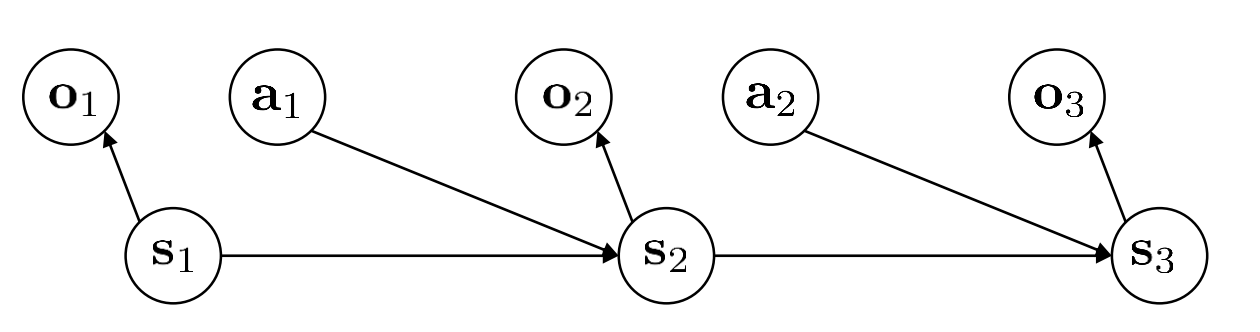
\includegraphics[scale = 0.4]{figures/markov.png}
    \caption{A simple Markov chain.}
    \label{fig:markov}
\end{figure}

In control theory, such as the LQR optimization problem, we aim to minimize the cost function of the system. What would be an equivalent notion in reinforcement learning? Recall we defined a reward function, $r(s,a)$, so naturally we want to collect as much reward as possible in the environment. Without loss of genrality, we assume that the environment is stochastic. Define a trajectory distribution $p_\theta(\tau)$ according to Baye's Rule:
$$ p(\tau) \vcentcolon= p(s_1,a_1,...,s_T,a_T) = p(s_1)\prod_{t=1}^T\pi_\theta(a_t|s_t)p(s_{t+1}|s_t,a_t)$$
where $T$ is the length of episode horizon. Therefore, given this trajectory distribution, we can calculate the expected value of the total reward function induced by following this trajectory as $\mathbb{E}_{\tau\sim p_\theta(\tau)}\left[\sum_t r(s_t,a_t)\right]$. Therefore, to optimize this objective, we want to find a parameter $\theta$, such that $\theta$ maximizes the above expectation:
$$\theta = \argminA_\theta\mathbb{E}_{\tau\sim p_\theta(\tau)}\left[\sum_t r(s_t,a_t)\right]$$
\section{Value Function and Q Function}
To facilitate our calculation of the above expectation, and to simplify the notations, we introduce two important types of functions: Q function and value function. In most cases these two functions are not given to us in closed form, and one needs to approximate and improve the functions using some deep neural net, hence the notion of ``deep'' in deep reinforcement learning.
\subsection{Q Function}
Q function is a function of both state and action, so it is denoted as $Q(s_t,a_t)$ and it quantitatively measures the quality of taking action $a_t$ at state $s_t$. Mathematically, it is the expected sum of reward from the current time step given state $s_t$ and action $a_t$. This is very similar to the ``cost-to-go'' function in control theory, especially Model Predictive Control. We define $Q(s,a)$ as:
$$Q^\pi(s_t,a_t) = \sum_{t'=t}^T{\mathbb{E}_{\pi_\theta}[r(s_t',a_t')|s_t,a_t]}$$
\subsection{Value Function}
Unlike the Q function, value function is only a function of state, so intuitively it quantitatively measures the value of being in state $s_t$. Mathematically, it is defined as $V^\pi(s_t) =\sum_{t'=t}^T{\mathbb{E}_{\pi_\theta}[r(s_t',a_t')|s_t]}$. Again by Baye's rule we can obtain the relation between Value function and Q function: $V^\pi(s_t)=\mathbb{E}_{a_t\sim\pi(a_t|s_t)}[Q^\pi(s_t,a_t)]$.

Furthermore, if we sum the value function over all possible initial states, we essentially recovered the objective of reinforcement learning: $\mathbb{E}_{s_1\sim p(s_1)[V^\pi(s_1)]}$, where $p(s_1)$ is a known distribution of all possible initial states.
\section{Reinforcement Learning Anatomy}
In RL, we usually have three parts in the whole pipeline. We need to keep generating data for the agent to learn, and use the data to generate samples in order to fit and regress onto a model. Then with this model, we estimate the reward and based on the reward we update our policy to maximize the reward, and we go back to step 1. Therefore, our primal concern is to efficiently run the three parts so that the agent can learn optimally with less data and computation. Here is an illustration of the three steps in Fig. \ref{fig:rlanatomy}.
\begin{figure}
    \centering
    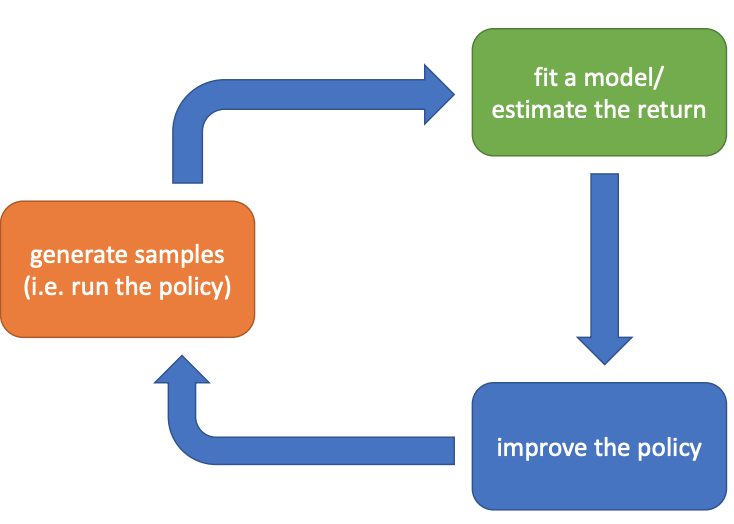
\includegraphics[scale=0.5]{figures/rlanatomy.png}
    \caption{Three steps of reinforcement learning.}
    \label{fig:rlanatomy}
\end{figure}
\chapter{Imitation Learning}
Imitation learning is also called behavioral cloning. The basic idea of imitation learning is ``train to fit the expert behavior''. In other words, given a demonstration, we want to make the agent follow the demonstration as closely as possible, to best imitate the demonstration's behaviors.
\section{Distribution Mismatch}
However, a big problem of such type of approach is that it does not generalize well, if at all. For example, one can imagine that the agent makes a small mistake and ends up being in a slightly different state that what it has seen (trained) before, but since the state is novel, the agent does not know how to act, thus behaving randomly, diverging from the learned trajectory. An illustration of such mismatches is shown in Fig. \ref{fig:imitation_div}.
\begin{figure}
    \centering
    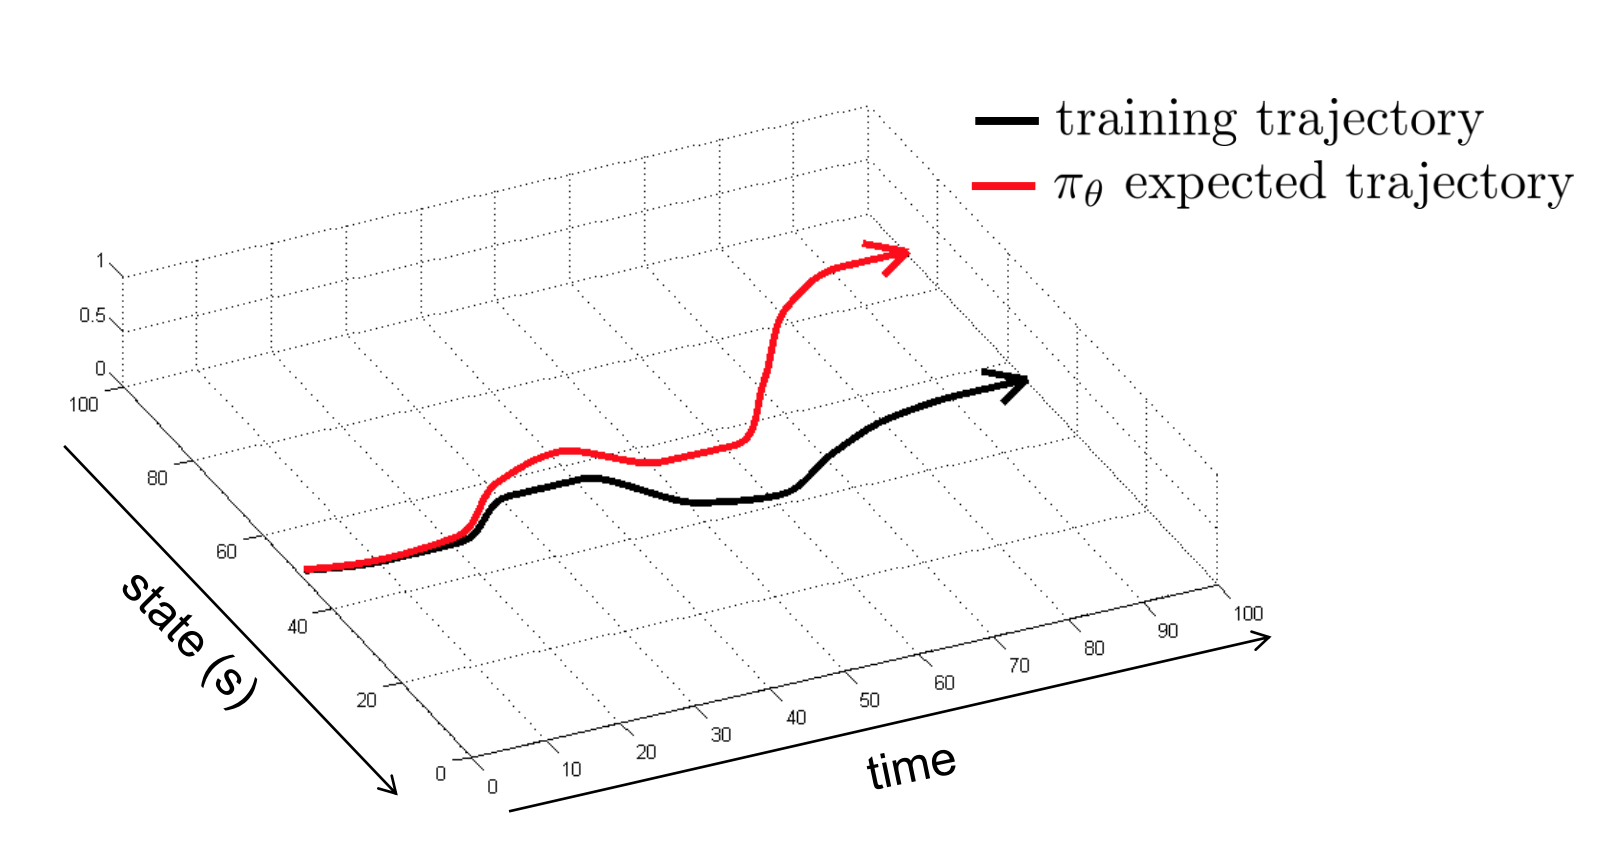
\includegraphics[scale = 0.3]{figures/imitation_div.png}
    \caption{Mistakes aggregate in behavior cloning.}
    \label{fig:imitation_div}
\end{figure}
\section{Dataset Aggregation}
The aggregation of mistakes that the agent makes often makes imitation learning not feasible. But imitation learning does work in some cases. Intuitively, if the agent could somehow learn from the mistakes, and we keep appending data to the agent's dataset so that the agent is exposed to a variety of states. If the actions applied to those states are correct, then eventually, the agent can, ideally, converge to an optimal trajectory. This is essentially the idea behind an imitation learning algorithm called Dataset Aggregation (DAgger) \cite{ross2011reduction}.
\begin{algorithm}[t!]
\caption{Dataset Aggregation (DAgger)}
\begin{algorithmic}[1]
\label{alg:dagger}
\REQUIRE Human data $\mathcal{D} = \{o_1,a_1,...,o_N,a_N\}$

\WHILE{true}
    \STATE Train $\pi_\theta(a_t|o_t)$ from human data $\mathcal{D} = \{o_1,a_1,...,o_N,a_N\}$.
    \STATE Run $\pi_\theta(a_t|o_t)$ to get dataset $\mathcal{D}_\pi = \{o_1,...,\o_M\}$
    \STATE Ask human to label $\mathcal{D}_\pi$ with actions $a_t$
    \STATE Aggregate $\mathcal{D} \leftarrow \mathcal{D} \cup \mathcal{D_\pi}$
\ENDWHILE
\RETURN optimal imitation-learned trajectory as $\tau^{return}$
\end{algorithmic}
\end{algorithm}
In step 3 of Algorithm \ref{alg:dagger}, what we are doing is basically discarding the actions from running trained policy $\pi_\theta(a_t|o_t)$. Instead, we ask a human in the loop to label what they would have done based on the observations in $D_\pi$. Take an autonomous car for example, the training data would be images labeled with steering commands, and we let the car collect more data, which are only images. Then we give those images to a human, and let the human determine, based on each image, what action (steer left, right, or go straight) that the human would have applied if he observed such an image.

It can be proven that DAgger resolves the distribution ``drift'' issue. However, one problem with DAgger is that human might be error-prone, so the human labelled data might be flawed to use. Furthermore, more subtly, human, in most cases, does not make decisions based on a Markovian process. Therefore, the current time step's action might be dependent on a state/observation some number of time steps ago.
\section{When Does Imitation Learning Fail?}
In general, there are some cases where one may fail to fit the expert data, which lead to undesirable outcomes of imitation learning.
\subsection{Non-Markovian Behaviors}
First, the data is Non-Markovian, as mentioned above. Actually Non-Markovian process is more natural and intuitive for human in that human learns from their past mistakes. Why is this wrong? Essentially, we are fitting the wrong distribution. Since we are fitting a policy distribution based on a Markovian process, our goal is fitting $\pi(a_t|o_t)$. However, if the expert data is not Markovian, then we are trying to fit $\pi(a_t|o_t)$ from another distribution $\pi(a_t|o+1,...,o_t)$. One solution is to use a lot of previous memory frames, and concatenate them as one huge frame, effectively augmenting the state space. However, this solution might generate too many weights, increasing the computation complexity. Another solution is that one can fit the expert data using an RNN with shared weights, and one possible implementation is shown in Fig. \ref{fig:im_RNN}.
\begin{figure}
    \centering
    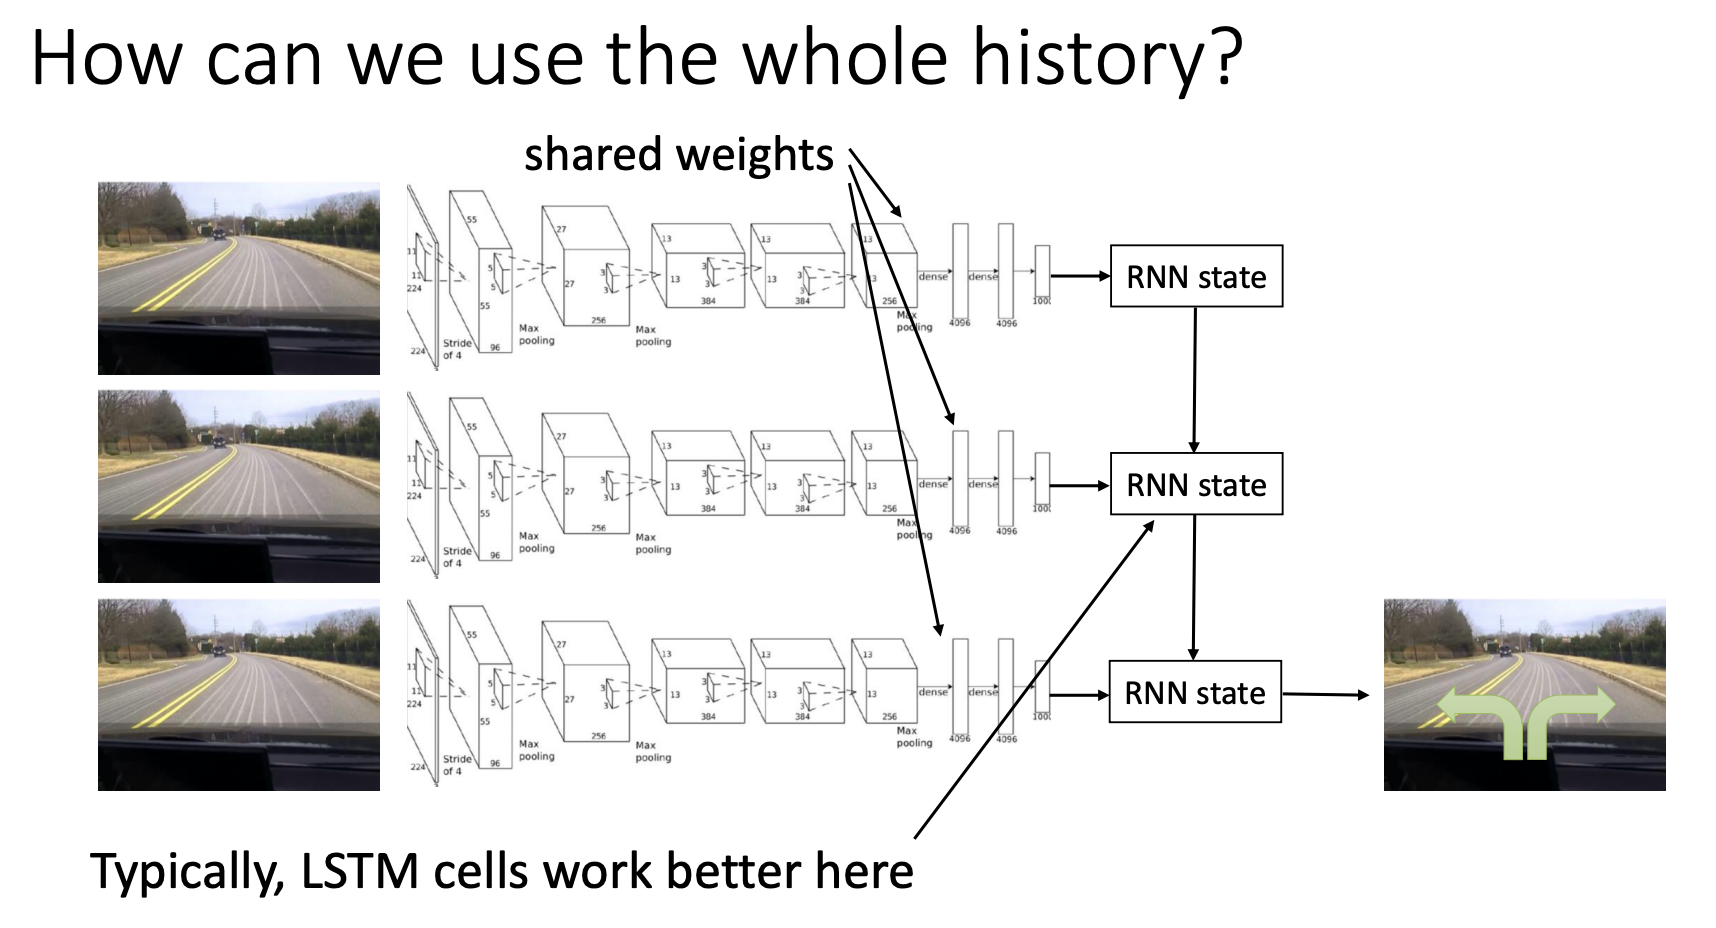
\includegraphics[scale = 0.4]{figures/im_RNN.png}
    \caption{Using RNN to address non-Markovian expert data.}
    \label{fig:im_RNN}
\end{figure}
The underlying reason why having a full history makes imitation learning difficult is that history data tends to exacerbate the causality misclassification. Having more history might make the agent learn the wrong direction of causality, and in many cases, the wrong direction is actually easier to learn. For more information, please refer to this paper \cite{de2019causal}.
\subsection{Multimodal Behaviors}
Another scenario where fitting expert might fail is that the expert has \textbf{multimodal} behaviors. An example of this is that when you are controlling a drone to dodge a tree ahead, you either steer left or steer right. However, if you choose the wrong parametric form of the distribution (e.g. a simple Gaussian) of the actions, the distribution might average out left and right and choose to go straight, as shown in figure \ref{fig:multimodal}.
\begin{figure}
    \centering
    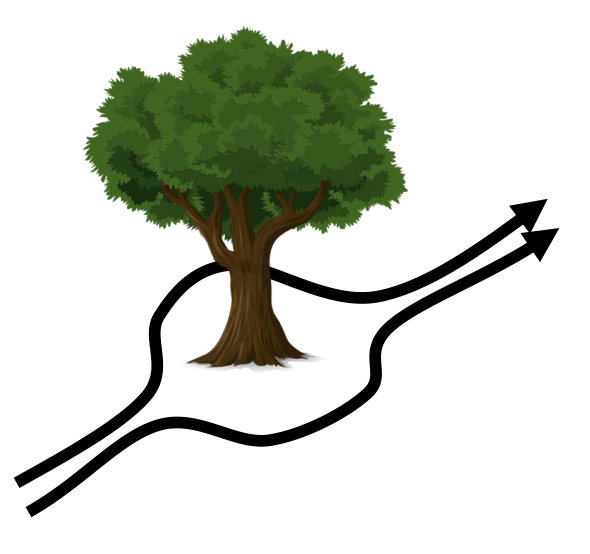
\includegraphics[scale=0.5]{figures/multimodal.png}
    \caption{Multimodal behaviors.}
    \label{fig:multimodal}
\end{figure}
Some methods to mitigate this issue include: first, one can use a mixture of different Gaussian distributions, instead of just one. Second, construct a latent space variables model, which we will talk more about in variational inference. Third, we can use autogregressive discretization. Specifically, a mixture of Gaussians means that the policy distribution should be a weighted sum of different Gaussians with different means and variances. 
\section{Theoretical Analysis of Imitation Learning's Error}
First we define two different reward functions for imitation learning. To make our analysis easier, we assume the policy function is deterministic. First, we can define the reward function as $r(s,a)=\log p(a=\pi^*(s)|s)$. This function measures the log likelihood of the action equal to expert policy's action. Another (simpler) choice can just be a counter to count the number of mistakes. Specifically, 
\[ c(s,a) = \begin{cases} 
          0 & \text{if } a = \pi^*(s) \\
          1 & \text{o.w.}
       \end{cases}
    \]
To analyze this, let's introduce a lower bound on the probability of making mistakes: $\pi_\theta(a\neq \pi^*(s)|s)\leq \epsilon$ for all $s\sim p_{train}(s)$. The fit distribution of states $p_\theta(s)$ is consisted of two parts: the first part is the probability of no mistakes made, and the second part is the probability of making some mistakes. Using Baye's rule, we can calculate $p_\theta(s)$ as follows:
$$p_\theta(s_t) = (1-\epsilon)^tp_{train}(s_t)+(1-(1-\epsilon)^t)p_{mistake}(s_t)$$
so to measure the divergence of $p_\theta$ from $p_{train}$, we take the difference of the two distriutions (naive):
$$|p_\theta(s_t)-p_{train}(s_t)|=(1-(1-\epsilon)^t)|p_{mistake}-p_{train}|\leq2(1-(1-\epsilon)^t)$$
$$\leq 2\epsilon t$$
where we used the identity that $(1-\epsilon)^t\geq1-\epsilon t$ for $\epsilon\in [0,1]$. Thus, we can calculate the expected number of mistakes the agent makes using this scheme by:
$$\sum_t\mathbb{E}_{p_\theta(s_t)}[c_t] = \sum_t\sum_{s_t}p_\theta(s_t)c_t(s_t)\leq\sum_t\sum_{s_t}p_{train}(s_t)c_t(s_t)+|p_\theta(s_t)-p_{train}(s_t)|c_{max}$$
$$\leq\sum_t\epsilon+2\epsilon t$$
$$\in O(\epsilon T^2)$$
Also note that with DAgger $p_{train}(s)\rightarrow p_\theta(s)$. So we no longer have the second item inside the summation for DAgger. Thus for dagger, the expected value should be in $O(\epsilon T)$.

As we see, when we have longer horizon length, the errors are going to be aggregated, thus making more mistakes, and this is one of the most fundamental disadvantages of imitation learning \cite{ross2011reduction}.
\section{Summary}
Overall, what are some disadvantages of imitation learning? We have a human factor to provide data in the entire loop, which is potentially finite, and to generate a good policy, one need to learn from a lot of data. Moreover, human cannot provide all kinds of data. Specifically, a human may have trouble with providing data such as the joint angle/torque of a robotic arm. Therefore, we wish that machines can learn automatically, from unlimited data.
\chapter{Policy Gradient Methods}
Recall the objective of Reinforcement Learning:
$$\theta = \argmaxA_\theta\mathbb{E}_{\tau\sim p_\theta(\tau)}\left[\sum_t r(s_t,a_t)\right]$$
This is actually framed as an optimization problem. Therefore, we can use a variety of optimization techniques, such as gradient descent, to optimize this objective. To be more concrete, let us define a function $J(\theta)$:
$$J(\theta) = \mathbb{E}_{\tau\sim \pi_\theta(\tau)}[r(\tau)]$$
By definition, $r(\tau)$ is the sum of reward incurred in this trajectory, so it can be equivalently defined as $\sum_{t=1}^T r(s_t,a_t)$, and by definition of expectation, we can more conveniently express the $J$ function as an integral of the product of policy and reward:
$$J(\theta) = \int \pi_\theta r(\tau)d\tau$$.
With this integral, we can easily take the gradient to perform gradient descent/ascent. A convenient expression of the gradient of $J(\theta)$ is shown below.
\section{Policy Gradient Theorem}
In this section, we will derive the mathematical expression of the policy gradient theorem.

Recall a convenient identity:
$$\pi_\theta(\tau)\nabla_\theta \log \pi_\theta(\tau) = \pi_\theta(\tau)\frac{\nabla_\theta \pi_\theta(\tau)}{\pi_\theta(\tau)}=\nabla \pi_\theta (\tau)$$
Using this identity, we can take the gradient of $J(\theta)$ in a cleaner fashion:
\begin{align*}
\nabla_\theta J(\theta) = \int \nabla_\theta \pi_\theta r(\tau)d\tau\\
=\int\pi_\theta(\tau)\nabla_\theta \log \pi_\theta(\tau) r(\tau) d\tau\\
= \mathbb{E}_{\tau\sim \pi_\theta(\tau)}[\nabla \log \pi_\theta (\tau)r(\tau)]
\end{align*}
Now, we want to get rid of the huge $\log \pi_\theta(\tau)$ from our equation. Recall that a trajectory $\tau$ is a list of states and actions, so $\pi_\theta(s_1,a_1,...,s_T,a_T) = p(s_1)\prod_{t=1}^T\pi_\theta (a_t|s_t)p(s_{t+1}|s_t,a_t)$ by Baye's rule. Then we take the log on both sides, and we end up getting $\log\pi_\theta(\tau) = \log p(s_1) + \sum_{t=1}^T \log\pi_\theta(a_t|s_t)+\log p(s_{t+1}|s_t,a_t)$.
Plugging into our original gradient:
\begin{equation}
\begin{aligned}
    \nabla_\theta J(\theta) &= \mathbb{E}_{\tau\sim \pi_\theta(\tau)}\left[\nabla_\theta\left(\log p(s_1) + \sum_{t=1}^T \log \pi_\theta(a_t|s_t)+\log p(s_{t+1}|s_t,a_t)\right)r(\tau)\right]\\
    &= \mathbb{E}_{\tau\sim \pi_\theta(\tau)}\left[ \left(\sum_{t=1}^T\nabla_\theta \log\pi_\theta(a_t|s_t)\right)\left(\sum_{t=1}^T r(s_t,a_t)\right)\right]
\end{aligned}
\end{equation}
Note that in the above calculation, we cancel out $\log p(s_1)$ and $\log p(s_{t+1}|s_t,a_t)$ because we are taking the gradient with respect to $\theta$, but those two expressions do not depend on $\theta$. The first item in the final expectation is similar to maximum likelihood.
\section{Evaluating the Policy Gradient}
In our derivation, we mathematically derived an expression for policy gradient. However, in most cases we cannot easily obtain the expectation easily because it is highly possible to involve a huge integral. Therefore, what are we going to do if the expectation (integral) is hard to evaluate? The answer is to approximate, and more specifically, we use Monte Carlo approximation. The idea is to take N samples, and average them out:
$$\nabla_\theta J(\theta) \simeq \frac{1}{N}\sum_{i=1}^N\left(\sum_{t=1}^T\nabla_\theta \log\pi_\theta(a_{i,t}|s_{i,t})\right)\left(\sum_{t=1}^T r(s_{i,t},a_{i,t})\right)$$
With the above gradient, we can do gradient descent (ascent) on the parameter $\theta$ by:
$$\theta \leftarrow \theta + \alpha\nabla_\theta J(\theta)$$ Now we are ready to propose a vanilla policy gradient algorithm by direct gradient ascent on the Monte Carlo-approximated policy gradient parameters, the REINFORCE Algorithm, as shown in Algorithm \ref{alg:reinforce}.
\begin{algorithm}[t!]
\caption{REINFORCE Algorithm}
\begin{algorithmic}[1]
\label{alg:reinforce}
\REQUIRE Base policy $\pi_\theta(a_t|s_t)$, sample trajectories $\tau^i$

\WHILE{true}
    \STATE Sample $\{\tau^i\}$ from $\pi_\theta(a_t|s_t)$ (run it on a robot).
    \STATE $\nabla_\theta J(\theta) \simeq \frac{1}{N}\sum_i\left(\sum_t\nabla_\theta \log\pi_\theta(a_{i,t}|s_{i,t})\right)\left(\sum_t r(s_{i,t},a_{i,t})\right)$
    \STATE Improve policy by $theta \leftarrow \theta + \alpha\nabla_\theta J(\theta)$
\ENDWHILE
\RETURN optimal trajectory from gradient ascent as $\tau^{return}$
\end{algorithmic}
\end{algorithm}

\section{Example: Gaussian Policy}
Now let us work out a simple case of running Algorithm \ref{alg:reinforce} on a simple Gaussian policy. A Gaussian policy means that the policy function is a Gaussian distribution. Specifically, $\pi_\theta(a_t|s_t) = \mathcal{N}\left(f_\text{neural net}(s_t); \Sigma\right)$. One advantage of using a Gaussian policy is that it is easy to obtain a closed-form expression for the Gaussian derivative:
$$\log \pi_\theta(a_t|s_t) = -\frac{1}{2}{\left\lVert f(s_t)-a_t\right\rVert}_\Sigma^2 + C$$
Taking the derivative, we have:
$$\nabla_\theta \log \pi_\theta(a_t|s_t) = -\frac{1}{2}\Sigma^{-1}(f(s_t)-a_t)\frac{df}{d\theta}$$
And we use Gradient ascent as discussed above.
\section{Intuition behind Policy Gradient: What are We Actually Doing?}
Recall we mentioned that the first term inside the expectation is similar to maximum likelihood. Let us compare the two side by side. Recall the expression of the policy gradient is:
$$\nabla_\theta J(\theta) \simeq \frac{1}{N}\sum_{i=1}^N\nabla_\theta \log \pi_\theta(\tau_i)r(\tau_i)$$
And the Maximum Likelihood is defined as:
$$\nabla_\theta J_{ML}(\theta)\simeq\frac{1}{N}\sum_{i=1}^N\nabla_\theta \log \pi_\theta(\tau_i)$$
As we discussed before, the first term in the policy gradient is exactly the same as the definition of maximum likelihood!

So what are we doing here when taking this gradient? Intuitively, we are assigning more weight to more rewarding trajectories by making trajectories with higher rewards more probable. Equivalently, higher-reward trajectories are likely to have more probability to be chosen. This intuition is crucial to the policy gradient methods and is illustrated in Fig. \ref{fig:trajheat}
\begin{figure}
    \centering
    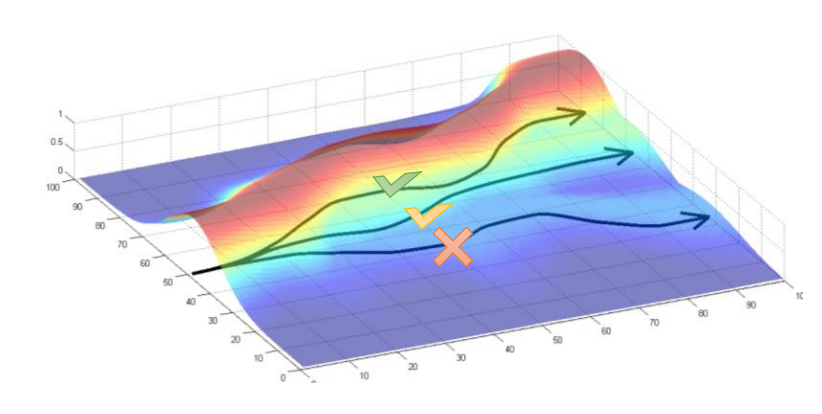
\includegraphics[scale=0.5]{figures/trajheat.png}
    \caption{More rewarding trajectories are more probable.}
    \label{fig:trajheat}
\end{figure}

\section{Partial Observability}
Can we use the policy gradient on a Partially Observed Markov Decision Process (POMDP)? The short answer is Yes. Why? Recall (yet again) the policy gradient expression:

$$\nabla_\theta J(\theta) \simeq \frac{1}{N}\sum_{i=1}^N\left(\sum_{t=1}^T\nabla_\theta \log\pi_\theta(a_{i,t}|s_{i,t})\right)\left(\sum_{t=1}^T r(s_{i,t},a_{i,t})\right)$$

In this expression, we do not even have the transition function in it. Long story short, the Markovian property is not actually used! So we can use policy gradient on a POMDP without any modification except instead of $s_t$, we use $o_t$.

Note that we do not care about what the state actually is. Any Non-Markovian proces can be made Markovian by setting the state as the whole history. 

\section{Disadvantages of the Policy Gradient}
Recall the intuition behind the policy gradient update: we make trajectories with more reward more probable. Let's consider the following scenario: say two trajectories have similar positive rewards, while another trajectory has a low, negative reward. Then policy gradient is going to assign zero to low probability to the third reward, and high probabilities to the other two. Now imagine we add a large constant number to our reward function, and apparently it does not change the relative relation between different trajectories' rewards because we are only adding in a constant. Now the negative reward becomes positive, and policy gradient is likely to spread out the likelihood for the three trajectories since all three rewards are positive now. This is bad because our reward does not change at all in fact, but after adding in a constant, the distribution of policy gradient changed substantially. 

Therefore, we need to come up with some methods to reduce the variance introduced in the policy gradients. 
\section{Reducing Policy Gradients Variance using Baselines}
\subsection{Causality}
One simple fix for high variance is to use the fact of causality: policy at time $t'$ cannot affect reward at $t$ if $t<t'$. This simple commonsensical idea allows us to discard some operands in the summation:
$$\nabla_\theta J(\theta) \simeq \frac{1}{N}\sum_{i=1}^N\left(\sum_{t=1}^T\nabla_\theta \log\pi_\theta(a_{i,t}|s_{i,t})\right)\left(\sum_{t'=t}^T r(s_{i,t'},a_{i,t'})\right)$$
and we define the second item in the summation as the ``reward-to-go''. Notice that in the reward-to-go term, we start the summation from time $t$ instead of 1, by causality. The idea is that we are multiplying the likelihood by smaller numbers due to the reduction of the summation term, so we can reduce the variance to some extent.
\subsection{Baselines}
Another common approach is to use baselines. By baselines, we mean that instead of making all high-reward trajectories more likely, we only make trajectories \textbf{better than average} more likely. So naturally, we define a baseline $b$ as the average reward:
$$b = \frac{1}{N} \sum_{i=1}^Nr(\tau)$$
Incorporating the baseline $b$ into our original policy gradient expression:
$$\nabla_\theta J(\theta) \simeq \frac{1}{N}\sum_{i=1}^N \nabla_\theta \log\pi_\theta(\tau)\left[r(\tau)-b\right]$$
But, are we allowed to that? Yes, in fact, we can show that the expectation is the same with baseline $b$. To show this, we can express the expectation of baseline as:
\begin{align*}
\mathbb{E}\left[\nabla_\theta\log \pi_\theta(\tau)b\right]&=
\int \pi_\theta(\tau)\nabla \log\pi_\theta(\tau)b\;d\tau\\
&=\int \nabla_\theta \pi_\theta(\tau)b\;d\tau\\
&=b\nabla_\theta\int\pi_\theta(\tau)\;d\tau\\
&=b\nabla_\theta 1\\
&=0
\end{align*}
Therefore, by subtracting a baseline, our policy gradient is still unbiased in expectation!
\subsection{Analyzing the Variance with Baselines}
Let us explicitly write down the variance of the policy gradient. Recall the definition of variance:
$$\mathrm{Var}[x] = \mathbb{E}[x^2]-\mathbb{E}[x]^2$$
And the policy gradient with baselines is written as:
$$\nabla_\theta J(\theta) \simeq \mathbb{E}_{\tau\sim\pi_\theta(\tau)}\left[\nabla_\theta \log\pi_\theta(\tau)\left(r(\tau)-b\right)\right]$$
Therefore, the variance of the policy gradient can be written as follows:
$$\mathrm{Var} = \mathbb{E}_{\tau\sim\pi_\theta(\tau)}\left[\left(\nabla_\theta \log\pi_\theta(\tau)\left(r(\tau)-b\right)\right)^2\right] - \mathbb{E}_{\tau\sim\pi_\theta(\tau)}\left[\nabla_\theta \log\pi_\theta(\tau)\left(r(\tau)-b\right) \right]^2$$
Note that in the second expectation term of variance, it can be equivalently written as $\mathbb{E}_{\tau\sim\pi_\theta(\tau)}\left[\nabla_\theta \log\pi_\theta(\tau)r(\tau) \right]^$ since baselines are unbiased in expectation.

Now we have an expression of variance with respect to baseline $b$, we can calculate the optimal $b$ that minimizes the variance by setting the gradient of variance to 0:
\begin{align*}
    \frac{d\mathrm{Var}}{db} &= \frac{d}{db}\mathbb{E}\left[g(\tau)^2(r(\tau)-b)^2\right]\\ &=\frac{d}{db}\mathbb{E}\left[g(\tau)^2r(\tau)^2\right] - 2\mathbb{E}\left[g(\tau)^2r(\tau)b\right] + b^2\mathbb{E}\left[g(\tau)^2\right]\\
    &=-2\mathbb{E}\left[ g(tau)^2r(\tau)\right]+2b\mathbb{E}\left[g(\tau)^2\right]\\
    &=0
\end{align*}
Solving the equation, we will have
$$b^{opt} = \frac{\mathbb{E}\left[g(\tau)^2r(\tau)\right]}{\mathbb{E}\left[g(\tau)^2\right]}$$
where $b^{opt}$ is the optimal baseline value for reducing the variance.

In practice, we just use the average reward for baseline. 

\section{On-Policy vs. Off-Policy}
We now introduce two concepts in RL: on-policy and off-policy. On-policy means that we learn only from using the current policy $\pi_\theta$, and off-policy means we learn also from other policies. Apparently, policy gradient is an on-policy method because $\nabla_\theta J(\theta) \simeq \mathbb{E}_{\tau\sim\pi_\theta(\tau)}\left[\nabla_\theta \log\pi_\theta(\tau)\left(r(\tau)-b\right)\right]$, and the expectation is taken under the current, known trajectory of interest. Therefore, every time we have a new policy, we need to use new samples. Since we are changing $\theta$, $\pi_\theta$ also changes overtime in policy gradient. One can imagine that this is extremely inefficient in neural networks, because in a neural network, $\theta$ only changes a little and the overhead for changing the policy is large.

One solution is to use off-policy learning.

\subsection{Off-policy Learning and Importance Sampling}
We first introduce an important technique called importance sampling. Given a distribution $p(x)$, how do we calculate the expectation from samples from another distribution $q(x)$? This is the idea of importance sampling, by using an importance ratio, we can calculate the expectation from another distribution, this enabling to learn off-policy. 

In importance sampling:
\begin{align*}
    \mathbb{E}_{x\sim p(x)}\left[f(x)\right] &= \int p(x)f(x)\;dx\\
    &=\int \frac{q(x)}{p(x)}f(x)\;dx\\
    &=\mathbb{E}_{x\sim q(x)}\left[\frac{p(x)}{q(x)}f(x)\right]
\end{align*}

Then we can plug it into the off-policy policy gradient. Say we have a trained policy $\pi_\theta(\tau)$, and we have samples from another policy $\Bar{\pi}(\tau)$, we can use the samples from $\Bar{\pi}(\tau)$ to calculate $J(\theta)$ function using importance sampling:
\begin{align*}
    J(\theta) &= \mathbb{E}_{\tau\sim\pi_\theta(\tau)}\left[r(\tau)\right]\\
    &= \mathbb{E}_{\tau\sim\Bar{\pi}(\tau)}\left[ \frac{\pi_\theta(\tau)}{\Bar{\pi}(\tau)} r(\tau)\right]
\end{align*}
Now we want to look closely at the importance ratio. Recall that $\pi_\theta(\tau) = p(s_1)\prod_{t=1}^T\pi_\theta(a_t|s_t)p(s_{t+1}|s_t,a_t)$. Then we can simplify the ratio in the following way:
\begin{align*}
\frac{\pi_\theta(\tau)}{\Bar{\pi}(\tau)} &=\frac{p(s_1)\prod_{t=1}^T\pi_\theta(a_t|s_t)p(s_{t+1}|s_t,a_t)}{p(s_1)\prod_{t=1}^T\Bar{\pi}(a_t|s_t)p(s_{t+1}|s_t,a_t)}\\
&= \frac{\prod_{t=1}^T\pi_\theta(a_t|s_t)}{\prod_{t=1}^T\Bar{\pi}(a_t|s_t)}
\end{align*}
\subsection{Deriving Policy Gradient with Importance Sampling}
It turns out that we can recover the original policy gradient theorem using off-policy learning using importance sampling. Recall the objective of RL as defined in the first chapter:
$$\theta^* = \argmaxA_\theta J(\theta)$$
and we defined $J(\theta)$ as $J(\theta) = \mathbb{E}_{\tau\sim\pi_\theta(\tau)}\left[r(\tau)\right]$. Now if we want to estimate $J$ with some new parameter $\theta'$, we can use importance sampling as discussed above:
$$J(\theta') = \mathbb{E}_{\tau\sim\pi_\theta(\tau)}\left[\frac{\pi_{\theta'}(\tau)}{\pi_\theta(\tau)}r(\tau)\right]$$
then we take the gradient as:
$$\nabla_{\theta'}J(\theta') &= 
    \mathbb{E}_{\tau\sim\pi_\theta(\tau)}\left[\frac{\nabla_{\theta'}\pi_{\theta'}(\tau)}{\pi_\theta(\tau)}r(\tau)\right]\\
    &=\mathbb{E}_{\tau\sim\pi_\theta(\tau)}\left[\frac{\pi_{\theta'}(\tau)}{\pi_\theta(\tau)}\nabla_{\theta'}\log \pi_{\theta'}(\tau)r(\tau)\right]
$$

Now if we estimate it locally, by setting $\theta = \theta'$, then we will cancel out the importance ratio, ending up with $\mathbb{E}_{\tau\sim\pi_\theta(\tau)}\left[\nabla_{\theta'}\log \pi_{\theta'}(\tau)r(\tau)\right]$.

\section{First Order Approximation for Importance Sampling}
Now we focus on the cases where we do not use local approximation, when $\theta \neq \theta'$.
\begin{align*}
    J(\theta') &= \mathbb{E}_{\tau\sim\pi_\theta(\tau)}\left[r(\tau)\right]\\
    \nabla_{\theta'}J(\theta')&=\mathbb{E}_{\tau\sim\pi_\theta(\tau)}\left[\frac{\pi_{\theta'}(\tau)}{\pi_\theta(\tau)}\nabla_{\theta'}\log\pi_{\theta'}(\tau)r(\tau)\right]\\
    &= \mathbb{E}_{\tau\sim\pi_\theta(\tau)}\left[  \left(  \frac{\prod_{t=1}^T\pi_{\theta'}(a_t|s_t)}{\prod_{t=1}^T\pi_{\theta}(a_t|s_t)} \right)\left( \sum_{t=1}^T\nabla_{\theta'}\log\pi_{\theta'}(a_t|s_t)  \right)\left(\sum_{t=1}^Tr(s_t,a_t)\right)  \right]
\end{align*}
Now there is a problem in the equation. Note that the ratio of the two products can be very small or very big if $T$ is big, thus increasing the variance. To alleviate the issue, one can make use of causality as we discussed before:
\begin{align*}
    \nabla_{\theta'}J(\theta')&= \mathbb{E}_{\tau\sim\pi_\theta(\tau)}\left[  \left(  \frac{\prod_{t=1}^T\pi_{\theta'}(a_t|s_t)}{\prod_{t=1}^T\pi_{\theta}(a_t|s_t)} \right)\left( \sum_{t=1}^T\nabla_{\theta'}\log\pi_{\theta'}(a_t|s_t)  \right)\left(\sum_{t=1}^Tr(s_t,a_t)\right)  \right]\\
    &=\mathbb{E}_{\tau\sim\pi_\theta(\tau)}\left[  \sum_{t=1}^T\nabla_{\theta'}\log\pi_{\theta'}(a_t|s_t) \left(\prod_{t'=1}^T \frac{\pi_{\theta'}(a_{t'}|s_{t'}) }{\pi_{\theta}(a_{t'}|s_{t'})}\right)    \left(  \sum_{t'=t}^Tr(s_{t'},a_{t'})\left(  \prod_{t'' = t}^{t'}\frac{\pi_{\theta'}(a_{t''}|s_{t''}) }{\pi_{\theta}(a_{t''}|s_{t''})} \right)    \right)\right]
\end{align*}
Here we used the fact of causality that future actions don't affect the current weight. Also note that the last ratio of products can be deleted, and we essentially get the policy iteration algorithm, which we will discuss in later chapters. 

So when we delete the last weight, we end up having
$$\nabla_{\theta'}J(\theta')= \mathbb{E}_{\tau\sim\pi_\theta(\tau)}\left[   \sum_{t=1}^T\nabla_{\theta'}\log\pi_{\theta'}(a_t|s_t)    \left(\prod_{t'=1}^T \frac{\pi_{\theta'}(a_{t'}|s_{t'}) }{\pi_{\theta}(a_{t'}|s_{t'})}\right)\left(  \sum_{t'=t}^Tr(s_{t'},a_{t'})\right)\right]$$
The product of ratio is again exponential in $T$, so we may have high variance. 

Recall on-policy policy gradient:
$$\nabla_{\theta}J(\theta) \simeq \frac{1}{N} \sum_{i=1}^T \sum_{t=1}^T\nabla_\theta \log \pi_\theta(a_{i,t}|s_{i,t})\hat{Q}_{i,t}$$
Similarly in off-policy policy gradient:
\begin{align*}
    \nabla_{\theta'}J(\theta') &= \frac{1}{N} \sum_{i=1}^T \sum_{t=1}^T   \frac{\pi_{\theta'}(s_{i,t},a_{i,t})}{\pi_{\theta}(s_{i,t},a_{i,t})}\nabla_{\theta'} \log \pi_{\theta'}(a_{i,t}|s_{i,t})\hat{Q}_{i,t}\\
    &= \frac{1}{N} \sum_{i=1}^T \sum_{t=1}^T \frac{\pi_{\theta'}(s_{i,t})}{\pi_{\theta}(s_{i,t})}\frac{\pi_{\theta'}(s_{i,t}|a_{i,t})}{\pi_{\theta}(s_{i,t}|a_{i,t})}\nabla_{\theta'} \log \pi_{\theta'}(a_{i,t}|s_{i,t})\hat{Q}_{i,t}
\end{align*}
In later chapters, we can see that we can pretty much ignore the first states priors ratio.
\chapter{Actor-Critic Algorithms}
Recall from last chapter, we derived the policy gradient theorem:
$$\nabla_\theta J(\theta) \simeq \frac{1}{N}\sum_{i=1}^N\left(\sum_{t=1}^T\nabla_\theta \log\pi_\theta(a_{i,t}|s_{i,t})\right)\left(\sum_{t'=1}^T r(s_{i,t'},a_{i,t'})\right)$$
where we defined the summed reward as the ``reward-to-go'' function $\hat{Q}_{i,t}$, and it represents the estimate of expected reward if we take action $a_{i,t}$ in state $s_{i,t}$. We have shown that this estimate has very high variance, and we shall see how we can improve policy gradients from using better estimation of the reward-to-go function.

\section{Reward-to-Go}
Let us take a closer look at the reward-to-go. To improve the estimation, one way is to get closer to the precise value of the reward-to-go. We can define the reward-to-go using expectation:
$$Q(s_t,a_t) = \sum_{t'=t}^T \mathbb{E}_{\pi_\theta}\left[r(s_{t'},a_{t'})|s_t,a_t\right]$$
this is the \textbf{true, expected} value of the reward-to-go.

Therefore, one could imagine using this true expected value, combined with our original Monte Carlo approximation to yield a better estimate:
$$\nabla_\theta J(\theta) \simeq \frac{1}{N}\sum_{i=1}^N\sum_{t=1}^T\nabla_{\theta}\log \pi_\theta (a_{i,t}|s_{i,t})Q(s_{i,t},a_{i,t})$$.

\section{Using Baselines}
As we have seen in last chapter, one can reduce the high variance of the policy gradient using baselines. We have also seen that it is possible to calculate the optimal baseline value to yield the minimum variance, although people often use the average reward for sake of simplicity.

Motivated by this, let us recall the definition of the value function (defined in the introduction section):
$$V(s_t) = \mathbb{E}_{a_t\sim \pi_\theta(a_t|s_t)}\left[Q(s_t,a_t)\right]$$
By definition, the value function is the average of Q-function value.

Similarly, we can use the \textbf{average} reward-to-go as a baseline to reduce the variance. Specifically, we could use the value function $V(s_t)$ as the baseline, thus improving the estimate of the gradient in the following way:
$$\nabla_\theta J(\theta) \simeq \frac{1}{N}\sum_{i=1}^N\sum_{t=1}^T\nabla_{\theta}\log \pi_\theta (a_{i,t}|s_{i,t})\left(Q(s_{i,t},a_{i,t}) - V(s_{i,t})\right)$$
and the value function we used is a better approximation of the baseline $b_t = \frac{1}{N}\sum_i Q(s_{i,t},a_{i,t})$.

What have we done here? What is the intuition behind subtracting the value function from the Q-function? Essentially, we are quantifying how much an action $a_{i,t}$ is better than the average actions. In some sense, it measures the \textbf{advantage} of applying an action over the average action. Therefore, to formalize our intuition, let us define the advantage as follows:
$$A^\pi(s_t,a_t) = Q^\pi(s_t,a_t) - V^\pi(s_t)$$
which quantitatively measures how much better action $a_t$ is.

Putting it all together, now a better baseline-backed policy gradient estimate using Monte Carlo estimate can be written as:
$$\nabla_\theta J(\theta) \simeq \frac{1}{N}\sum_{i=1}^N\sum_{t=1}^T\nabla_{\theta}\log \pi_\theta (a_{i,t}|s_{i,t})A^\pi(s_{i,t},a_{i,t})$$.

\section{Value Function Fitting}
The better the estimate of the advantage function, the lower the variance, and we can have better policy gradient. Let us massage the definition of the Q-function a little in order to find some interesting mathematical relations between $Q$ and $V$:
\begin{align*}
    Q^\pi(s_t,a_t) &= \sum_{t'=t}^T \mathbb{E}_{\pi_\theta}\left[r(s_{t'},a_{t'})|s_t,a_t\right]\\
    &= r(s_t,a_t)+\sum_{t'=t+1}^T \mathbb{E}_{\pi_\theta}\left[r(s_{t'},a_{t'})|s_t,a_t\right]\\
    &= r(s_t,a_t) + V^\pi(s_{t+1})\\
    &= r(s_t,a_t) + \mathbb{E}_{s_{t+1}\sim p(s_{t+1}|s_t,a_t)}\left[V^\pi(s_{t+1})\right]
\end{align*}
The last expectation of the value function is used because we do not know what the next state actually is. Note that we can be a little crude with respect to that expectation in such a way that we just use the full value function $V^\pi(\cdot)$ on one single sample of the next state, and use the value as the expectation, ignoring the fact that there are multiple other next states. With this estimate, we can plug into the advantage function:
$$A^\pi(s_t,a_t) \simeq r(s_t,a_t) + V^\pi(s_{t+1}) - V^\pi(s_t)$$

Therefore, it is almost enough to just approximate the value function, which solely depends on state, to generate approximations of other functions. To achieve this, we can use a neural network to fit our value function $V(s)$, and use the fit value function to approximate our policy gradient, as illustrated in Fig. \ref{fig:fitV} 
\begin{figure}
    \centering
    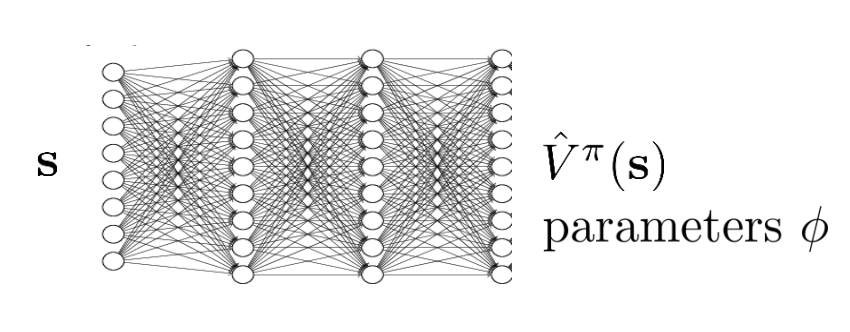
\includegraphics[scale=0.5]{figures/fitV.png}
    \caption{Fitting the value function}
    \label{fig:fitV}
\end{figure}

\section{Policy Evaluation}
Here in this section, we discuss the process and purpose of fitting the value function.

\subsection{Why Do We Evaluate a Policy}
Policy evaluation is a process that given a fixed policy $\pi$, we figure out how good it is by fitting the value function $V^\pi(\cdot)$ by using this expectation:
$$V^\pi(s_t) = \sum_{t'=t}^T\mathbb{E}_{\pi_\theta}\left[r(s_{t'},a_{t'})|s_t\right]$$
Having the value function allows us to figure out how good the policy is because the reinforcement learning objective can be equivalently written as $J(\theta) = \mathbb{E}_{s_1\sim p(s_1)}\left[V^\pi(s_1)\right]$, where we take the expectation of the value function value of the initial state over all possible initial states.
\subsection{How to Evaluate a Policy}
To evaluate a policy, we can use an approach similar to the policy gradient - Monte Carlo approximation. Specifically, we can estimate the value function by summing up the reward collected from time step $t$:
$$V^\pi(s_t) \simeq \sum_{t'=t}^T r(s_{t'},a_{t'})$$
and if we are able to reset the simulator, we could indeed ameliorate this estimate by taking multiple samples ($N$) as follows:
$$V^\pi(s_t) \simeq \frac{1}{N}\sum_{i=1}^N\sum_{t'=t}^T r(s_{i,t'},a_{i,t'})$$
In practice, we can just use the single sample approximation.

Here is a question, if our original objective is to use $V^\pi$ to reduce the variance, but we end up using a single sample estimation to estimate $V^\pi$, does it actually help? The answer is yes, because we are using a neural net to fit the Monte Carlo targets from a variety of different states, so even though we do single sample estimate, the value function does generalize when we visit similar states. 

\subsection{Monte Carlo Evaluation with Function Approximation}
To fit our value function, we could use a supervised learning approach. Essentially, we can use our single sample estimation of the value function as our function value, and fit a function that maps the states to the value function values. Therefore, our training data will be $\left\{(s_{i,t}, \sum_{t'=t}^Tr(s_{i,t'},a_{i,t'}))\right\}$, and we denote the function value labels as $y_{i,t}$, and we define a typical supervised regression loss function which we try to minimize as $\mathcal{L}(\phi) = \frac{1}{2}\sum_i\lvert|\hat{V}_\phi^\pi(s_i)-y_i|\rvert^2$. 

\subsection{Improving the Estimate Using Bootstrap}
In fact, we can improve our training process because the original applied target $y_{i,t}$ is not perfect. We could use a technique called bootstrapping. Recall the definition of our ideal target in the supervised regression:
$$\begin{aligned}
    y_{i,t} &= \sum_{t'=t}^T\mathbb{E}_{\pi_\theta}\left[r(s_{t'},a_{t'})|s_{i,t}\right]\\
    & \simeq r(s_{i,t},a_{i,t})+\sum_{t'=t+1}^T\left[r(s_{t'},a_{t'})|s_{i,t+1}\right]\\
    & \simeq  r(s_{i,t},a_{i,t}) + V^\pi(s_{i,t+1})
\end{aligned}$$
, compared with our Monte Carlo targets: $y_{i,t} = \sum_{t'=t}^T r(s_{i,t'},a_{i,t'})$.

Bootstrapping means applying our previous estimation on our current estimation. In our ideal targets, the last estimation is accurate if we knew the actual $V^\pi$. But if the actual is not known, we can just apply bootstrapping by using the current fit estimate $\hat{V}^\pi_\phi$ to estimate the next state's value: $\hat{V}^\pi_\phi(s_{i,t+1})$. Such an estimate is biased, but it has low variance.

Consequently, our training data using bootstrapping becomes: $\left\{(s_{i,t}, r(s_{i,t},a_{i,t}) +\hat{V}^\pi_\phi(s_{i,t+1})) \right\}$. Such bootstrapped targets work well with highly stochastic environments. 

\section{Batch Actor-Critic Algorithm}
Now we are ready to devise our first actor-critic algorithm. The reason why we call it actor-critic is that we use a critic (value function) to decrease the high variance of the actor (Q-function). The full algorithm is shown in Alg. \ref{alg:batchac} and we call it a batch algorithm because it is not online. We shall see the online version later.
\begin{algorithm}[t!]
\caption{Batch Actor-Critic Algorithm}
\begin{algorithmic}[1]
\label{alg:batchac}
\REQUIRE Base policy $\pi_\theta(a_t|s_t)$

\WHILE{true}
    \STATE Sample $\{s_i,a_i\}$ from $\pi_\theta(a|s)$ (run it on a robot)
    \STATE Fit $\hat{V}_\phi(s)$ to sampled reward sums
    \STATE Evaluate $\hat{A}^\pi(s_i,a_i) = r(s_i,a_i)+\hat{V}_\phi(s'_i)-\hat{V}_\phi(s_i)$
    \STATE $\nabla_\theta J(\theta) \simeq \sum_i\nabla_\theta\log \pi_\theta(a_i|s_i)\hat{A}^\pi(s_i,a_i)$
    \STATE Improve policy by $theta \leftarrow \theta + \alpha\nabla_\theta J(\theta)$
\ENDWHILE
\RETURN optimal policy from gradient ascent as $\pi^{return}$
\end{algorithmic}
\end{algorithm}
In Algorithm \ref{alg:batchac}, the way how we fit $\hat{V}_\phi$ is by minimizing the supervised regression norm $\mathcal{L}(\phi) = \frac{1}{2}\sum_i\lvert|\hat{V}_\phi^\pi(s_i)-y_i|\rvert^2$.
\section{Aside: Discount Factors}
Imagine if we had an infinite horizon environment ($T\rightarrow\infty$, then our estimated value function $\hat{V}^\pi_\phi(s)$ can get infinitely large in many cases. Therefore, one possible way to address this issue is to say that it is better to get rewards sooner than later. Therefore, instead of labeling our values as $y_{i,t} \simeq r(s_{i,t}, a_{i,t}) + \hat{V}^\pi_\phi(s_{i,t+1})$, we can shrink the value function value as we progress to the next time step. To achieve this, we introduce a hyperparameter called a \textbf{discount factor}, denoted as $\gamma$, where $\gamma \in [0,1]$:
$$y_{i,t} \simeq r(s_{i,t}, a_{i,t}) + \gamma\cdot\hat{V}^\pi_\phi(s_{i,t+1})$$
in most cases, $\gamma = 0.99$ works well.

Let us apply the discount factor to policy gradients. Basically, we have two options to impose this discount factor. The first option is :
$$\nabla_\theta J(\theta) \simeq \frac{1}{N}\sum_{i=1}^N\left(\sum_{t=1}^T\nabla_\theta \log\pi_\theta(a_{i,t}|s_{i,t})\right)\left(\sum_{t'=t}^T \gamma^{t'-t}r(s_{i,t'},a_{i,t'})\right)$$
and the second option is:
$$\begin{aligned}
\nabla_\theta J(\theta) &\simeq \frac{1}{N}\sum_{i=1}^N\left(\sum_{t=1}^T\nabla_\theta \log\pi_\theta(a_{i,t}|s_{i,t})\right)\left(\sum_{t=1}^T \gamma^{t-1}r(s_{i,t},a_{i,t})\right)\\
&\simeq \frac{1}{N}\sum_{i=1}^N\left(\sum_{t=1}^T\nabla_\theta \log\pi_\theta(a_{i,t}|s_{i,t})\right)\left(\sum_{t'=t}^T \gamma^{t'-1}r(s_{i,t'},a_{i,t'})\right) \;\mathrm{(causality)}\\
&\simeq \frac{1}{N}\sum_{i=1}^N\left(\sum_{t=1}^T\gamma^{t-1}\nabla_\theta \log\pi_\theta(a_{i,t}|s_{i,t})\right)\left(\sum_{t'=t}^T \gamma^{t'-t}r(s_{i,t'},a_{i,t'})\right)
\end{aligned}$$
Intuitively, the second option assigns less weight to later step's gradient, so it essentially means that later steps matter less in our discount. 

In practice, we can show that option 1 gives us better variance, so it is actually what we use. The full derivation can be found in this paper \cite{thomas2014bias}. Now in our actor-critic algorithm, after we impose the discount factor, we have the following gradient:
$$\nabla_\theta J(\theta) \simeq \frac{1}{N}\sum_{i=1}^N\left(\sum_{t=1}^T\nabla_\theta \log\pi_\theta(a_{i,t}|s_{i,t})\right)\left(r(s_{i,t},a_{i,t}) + \gamma\hat{V}_\phi^\pi(s_{i,t+1})-\hat{V}_\phi^\pi(s_{i,t})\right)$$

Now we can incorporate the discount factor with our actor-critic algorithm in Algorithm \ref{alg:batchacwdf}.
\begin{algorithm}[t!]
\caption{Batch Actor-Critic Algorithm with Discount Factor}
\begin{algorithmic}[1]
\label{alg:batchacwdf}
\REQUIRE Base policy $\pi_\theta(a_t|s_t)$, hyperparameter $\gamma$

\WHILE{true}
    \STATE Sample $\{s_i,a_i\}$ from $\pi_\theta(a|s)$ (run it on a robot)
    \STATE Fit $\hat{V}_\phi(s)$ to sampled reward sums
    \STATE Evaluate $\hat{A}^\pi(s_i,a_i) = r(s_i,a_i)+\gamma\hat{V}_\phi(s'_i)-\hat{V}_\phi(s_i)$
    \STATE $\nabla_\theta J(\theta) \simeq \sum_i\nabla_\theta\log \pi_\theta(a_i|s_i)\hat{A}^\pi(s_i,a_i)$
    \STATE Improve policy by $theta \leftarrow \theta + \alpha\nabla_\theta J(\theta)$
\ENDWHILE
\RETURN optimal policy from gradient ascent as $\pi^{return}$
\end{algorithmic}
\end{algorithm}

\section{Online Actor-Critic Algorithm}
Now that we have seen actor-critic algorithms with a batch of samples, we can further improve the performance by making it fully online. Namely, we are taking the gradient step based on the current sample so that we are not storing any large number of samples, which is more efficient. In the online version of actor-critic, we essentially use two neural nets: one for the policy, the other one for the value function. This is simple and stable, but as the states dimension becomes higher, we are not giving any shared features between the actor and the critic. Therefore, we can also make the network shared between the policy and the value function. In each step, we can only take one sample and gradually improve our value function using that sample. Here is the sketch of the online version of actor-critic algorithm in Algorithm \ref{alg:onlineac}. 
\begin{algorithm}[t!]
\caption{Online Actor-Critic Algorithm}
\begin{algorithmic}[1]
\label{alg:onlineac}
\REQUIRE Base policy $\pi_\theta(a_t|s_t)$, hyperparameter $\gamma$

\WHILE{true}
    \STATE Take action $a\sim\pi_\theta(a|s)$, get $(s,a,s',r)$
    \STATE Update $\hat{V}^\pi_\phi$ using target $r+\gamma\hat{V}^\pi_\phi(s')$
    \STATE Evaluate $\hat{A}^\pi(s,a)=r(s,a)+\gamma\hat{V}^\pi_\phi(s')-\hat{V}^\pi_\phi(s)$
    \STATE $\nabla_\theta J(\theta) \simeq \sum_i\nabla_\theta\log \pi_\theta(a|s)\hat{A}^\pi(s,a)$
    \STATE Improve policy by $theta \leftarrow \theta + \alpha\nabla_\theta J(\theta)$
\ENDWHILE
\RETURN optimal policy from gradient ascent as $\pi^{return}$
\end{algorithmic}
\end{algorithm}
Note that in steps 3-5, we are only taking a gradient step from one sample. In reality, this works best if we use a batch of samples instead of just one, and one can use parallel workers (simulations) either synchronously or asynchronously to achieve it, as illustrated in Fig \ref{fig:parallelsim}.
\begin{figure}
    \centering
    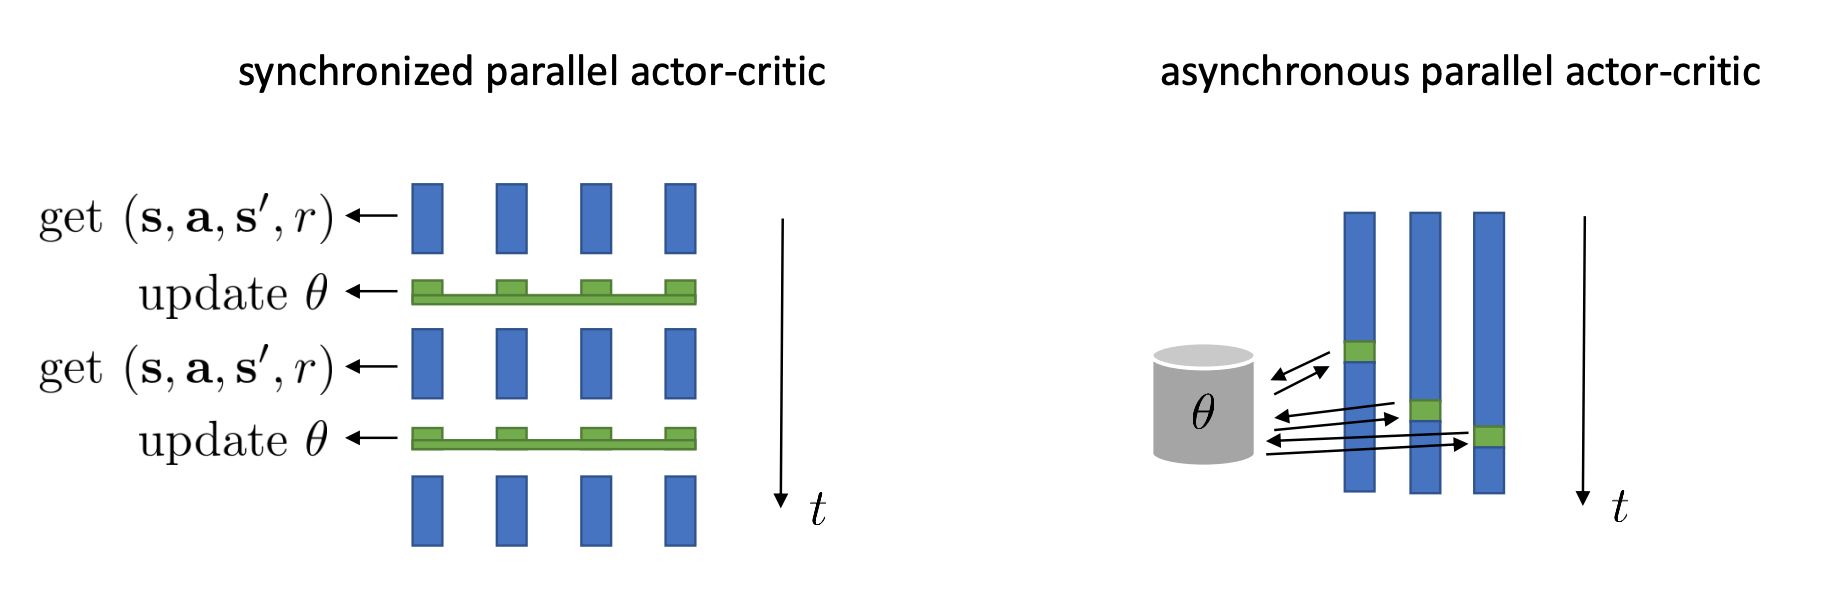
\includegraphics[scale=0.5]{figures/parallelsim.png}
    \caption{Parallel simulations for online actor-critic}
    \label{fig:parallelsim}
\end{figure}

\section{Critics as State-Dependent Baselines}
Now let us further discuss about the connection between a baseline and a critic. Recall in the Monte Carlo version of policy gradient, the gradient is defined as:
$$\nabla_\theta J(\theta) \simeq \frac{1}{N}\sum_{i=1}^N\left(\sum_{t=1}^T\nabla_\theta \log\pi_\theta(a_{i,t}|s_{i,t})\right)\left(\sum_{t'=1}^T r(s_{i,t'},a_{i,t'}) - b\right)$$
and in actor-critic algorithm, we estimate the gradient by estimating the advantage function:
$$\nabla_\theta J(\theta) \simeq \frac{1}{N}\sum_{i=1}^N\left(\sum_{t=1}^T\nabla_\theta \log\pi_\theta(a_{i,t}|s_{i,t})\right)\left(r(s_{i,t},a_{i,t}) + \gamma\hat{V}_\phi^\pi(s_{i,t+1})-\hat{V}_\phi^\pi(s_{i,t})\right)$$

So what are the pros and cons of the two approaches? In policy gradient with baselines, we have shown that there is no bias in our estimation, but there might be high variance due to our single-sample estimation of the cost-to-go function. On the other hand, in the actor-critic algorithm, we have shown that we have lower variance due to the critic, but we end up having a biased estimation because of the possibly bad critic as we are bootstrapping. So can we somehow keep the estimator unbiased while lowering the variance with the critic $\hat{V}^\pi_\phi$?

The solution is obvious and straightforward, we can just use $\hat{V}^\pi_\phi$ in place of $b$:
$$\nabla_\theta J(\theta) \simeq \frac{1}{N}\sum_{i=1}^N\left(\sum_{t=1}^T\nabla_\theta \log\pi_\theta(a_{i,t}|s_{i,t})\right)\left(\sum_{t'=1}^T r(s_{i,t'},a_{i,t'}) - \hat{V}^\pi_\phi(s_{i,t}))\right)$$
In this way, we obtain an unbiased estimator with lower variance. 

\section{Eligibility Traces and n-Step Returns}
In the above comparison of the two methods, we have seen that in the actor-critic advantage function, we have lower variance but higher bias, while in the Monte Carlo policy gradient, the advantage function has lower bias but higher variance. The reason why this tradeoff exists is that as we go further in our trajectory into the future, the variance increases due to the fact that the current single sample approximation is not representative enough for the future. Therefore, the Monte Carlo advantage function is good for getting accurate values in the near term, but not the long term. In contrast, in actor-critic advantage, the bias potentially skews the values in the near term, but the fact that the bias incorporates a lot of states will likely make it a better approximator in the long run. Therefore, it would be better if we could use the actor-critic based advantage for further in the future, and use the Monte Carlo based one for the near term in order to control the bias-variance tradeoff.

As a result, we can cut the trajectory before the variance gets too big. Mathematically, we can estimate the advantage function by combining the two approaches: use the Monte Carlo approach only for the first $n$ steps:
$$\hat{A}^\pi_n(s_t,a_t) = \sum_{t'=t}^{t+n}\gamma^{t'-t}r(s_{t'},a_{t'}) - \hat{V}^\pi_\phi(s_t)+\gamma^n\hat{V}^\pi_\phi(s_{t+n})$$
here we applied an n-step estimator, which sums the reward from now to $n$ steps from now, and $n>1$ often gives us better performance.

Furthermore, if we don't want to choose just one $n$, we can use a weighted combination of different $n$-steps returns, which we can define as the General Advantage Estimation(GAE):
$$ \hat{A}_{GAE}(s_t,a_t) = \sum_{n=1}^\infty w_n \hat{A}^\pi_n(s_t,a_t)$$
To choose the weights, we should prefer cutting earlier, so we can assign the weights accordingly: $w_n\propto \lambda^{n-1}$, where we call $\lambda$ the chance of getting cut.


\chapter{Value Function Methods}
In the last two chapters, we discussed some policy gradient-based algorithms. We have also seen the fact that the policy gradient methods have high variance. Therefore, it would be nice if we could completely omit the gradient step. To achieve this, we are going to talk about the value function methods in this chapter. 

\section{An Implicit Policy}
To omit the policy gradient, one still has to generate a policy function so that it takes in a state and outputs an action. Recall in actor-critic algorithms, we use the advantage function $A^\pi(s_t,a_t)$ to gauge how much better is the action $a_t$ than the average action according to $\pi$. Provided that we have a somehow accurate representation of this advantage function, we can just forget about generating a policy $\pi$, and just do this:
$$\argmaxA_{a_t} A^\pi(s_t,a_t)$$
which means we take the best action from $s_t$, if we follow $\pi$. Even though we have no knowledge of what the policy $\pi$ actually is, by doing the $\argmaxA$, we can guarantee that the action produced is at least as good as the action from the policy function that we do not know. Therefore, as long as we have a accurate representation of the advantage function $A^\pi(s_t,a_t)$, we can implicitly generate a parameter-free policy function:
\begin{align*}
\pi'(a_t|s_t) & = \begin{cases}
                1, & \mathrm{if } \;a_t = \argmaxA_{a_t}A^\pi(s_t,a_t)\\
                 0, & \mathrm{otherwise}
                    \end{cases}
\end{align*}
and as we have shown above, this implicit policy is at least as good as the unknown policy $\pi$.

\section{Policy Iteration}
Having omitted the policy, we can then proceed to introduce the policy iteration algorithm.
\subsection{High Level Idea}
The basic idea of policy iteration algorithms is very simple: we evaluate the advantage function $A^\pi(s,a)$ and then update the policy using the update rule as defined above in the implicit policy, and then we can loop to constantly improve our policy. 

The problem here is how to evaluate $A^\pi(s,a)$. In other words, how does one find an accurate representation of the advantage function in order to accurately update the policy. As before, we have seen that the advantage function an be equivalently defined as follows:
$$A^\pi(s,a) = r(s,a) + \gamma\mathbb{E}\left[V^\pi(s')\right]-V^\pi(s)$$
Therefore, if we can evaluate the value function $V^\pi(s)$ then we can also evaluate $A^\pi(s,a)$. So in the high-level policy iteration algorithm, we can just use the value function in place of the advantage function.

\subsection{Dynamic Programming}
Now let us make a simple assumption. Suppose we know a priori the transition probability $p(s'|s,a)$ and both states $s$ and action $a$ are discrete. Then a very natural dynamic programming update is the bootstrapped update, as we have seen before:
$$V^\pi(s)\leftarrow \mathbb{E}_{a\sim\pi(a|s)} \left[r(s,a) + \gamma\mathbb{E}_{s'\sim p(s'|s,a)}\left[V^\pi(s')\right]\right]$$
and we can just use the current estimate inside the nested expectation for simplicity. 

According to our definition of the implicit policy function $\pi'$, the policy is actually deterministic. Therefore, we can completely get rid of the outside expectation, and the value function update can be further simplified as:
$$V^\pi(s)\leftarrow r(s,\pi(s)) + \gamma\mathbb{E}_{s'\sim p(s'|s,a)}\left[V^\pi(s')\right]$$
\begin{algorithm}[t!]
\caption{Policy Iteration via DP}
\begin{algorithmic}[1]
\label{alg:policyiter1}
\WHILE{true}
    \STATE Evaluate $V^\pi(s,a)$
    \STATE Set $\pi\leftarrow \pi'$
\ENDWHILE
\end{algorithmic}
\end{algorithm}
This version of policy iteration is sketched in Algorithm \ref{alg:policyiter1}

We can even further simplify the dynamic programming update. Note that we in each iteration, we are updating the policy first in order to update the value function. Thus, it would be faster if we could skip the policy part and directly improve the value estimation. Meanwhile, the $\argmaxA$ operation that we apply on the advantage function itself is an implicit policy. We also know that $\argmaxA_{a_t}A^\pi(s,a) = \argmaxA_{a_t}Q^\pi(s,a)$, because the two values only differ by the subtraction term $V^\pi$, which does not depend on action:
$$A^\pi(s,a) = r(s,a) + \gamma\mathbb{E}\left[V^\pi(s')\right]$$
\begin{algorithm}[t!]
\caption{Value Iteration via DP}
\begin{algorithmic}[1]
\label{alg:policyiter2}
\WHILE{true}
    \STATE Set $Q(s,a)\leftarrow r(s,a) + \gamma\mathbb{E}\left[V(s')\right]$
    \STATE Set $V(s) \leftarrow \max_{a}Q(s,a)$
\ENDWHILE
\end{algorithmic}
\end{algorithm}
Having this, we can simplify the policy iteration algorithm further, as illustrated in Alg. \ref{alg:policyiter2}. As we skipped the policy update part, we call this new, simplified algorithm ``value iteration algorithm''.

\section{Fitted Value Iteration}
The policy iteration and value iteration algorithm we discussed above are heavily based on an impractical assumption: the total number of states is finite and small, because we are trying to construct a tabular expression of the value function and the Q function. Apparently, the tables are going to explode in dimensions if there are a lot of states. We call this the Curse of Dimensionality. To resolve this problem, we can use a neural network to approximate the functions instead of constructing a tabular expression of the function. 

\subsection{Fitted Supervised Value Iteration Algorithm}
Since we know that the value function is defined as $\max_a Q^\pi(s,a)$, we can use this definition as the labels for the value function in order to define a L2 loss function:
$$\mathcal{L}(\phi) = \frac{1}{2}\lvert|V_\phi(s) - \max_{a}Q^\pi(s,a)|\rvert^2$$
\begin{algorithm}[t!]
\caption{Fitted Value Iteration}
\begin{algorithmic}[1]
\label{alg:fittedvaliter}
\WHILE{true}
    \STATE set $y_i \leftarrow \max_{a_i}\left(r(s_i,a_i) + \gamma \mathbb{E}\left[V_\phi(s'_i)\right]\right)$
    \STATE set $\phi \leftarrow \argminA_\phi \frac{1}{2}\Sigma_i\lvert|V_\phi(s_i) - y_i|\rvert^2$
\ENDWHILE
\end{algorithmic}
\end{algorithm}
Then we can sketch out a simple fitted value iteration algorithm using this loss function in Algorithm \ref{alg:fittedvaliter}. Note that when setting the label, the ideal step to take is to enumerate all the states and find the corresponding label. However, when it is impractical, one could just use some samples and enumerate all the actions to find the labels. Moreover, when we take the maximum over all the actions from a state, we implicitly assume that the transition dynamics are known. Why? Because we want to take an action, record the value of that action, and then roll back to the previous state in order to check the values of other actions. Thus, without the transition dynamics, we cannot easily take the maximum.
\subsection{Fitted Q-Iteration Algorithm}
To address this problem, we can apply the same ``max'' trick in policy iteration. In policy iteration, we skip the policy update and calculate the values directly. Here in fitted value iteration, we can get around the transition dynamics by looking up the Q function table, because $V_\phi(s) \simeq \max_{a}Q_\phi(s,a)$, and this max operation is merely a table lookup from the Q value table. Consequently, we are now iterating on the Q values. Such a method works for off-policy samples (unlike actor-critic), and it only needs one network, so it does not have any high-variance policy gradient. However, as we shall see in later sections, such methods do not have convergence guarantees on non-linear functions, which could potentially be problematic.

The full fitted Q-iteration algorithm is shown in Algorithm \ref{alg:fittedQ}.
\begin{algorithm}[t!]
\caption{Fitted Q-Iteration Algorithm}
\begin{algorithmic}[1]
\label{alg:fittedQ}
\REQUIRE Some base policy for data collection; hyperparameter $K$
\WHILE{true}
    \STATE Collect dataset $\{(s_i,a_i,s'_i,r_i)\}$ using some policy
    \FOR{$K$ times}
        \STATE Set $y_i\leftarrow r(s_i,a_i) + \gamma \max_{a'_i}Q_\phi(s'_i,a'_i)$
        \STATE Set $\phi \leftarrow \argminA_\phi \frac{1}{2}\Sigma_i\lvert|Q_\phi(s_i,a_i) - y_i|\rvert^2$
    \ENDFOR
\ENDWHILE
\end{algorithmic}
\end{algorithm}
\subsection{A Closer Look at Q-Iteration Algorithm}
Let us take a closer look at the fitted Q-learning algorithm. 
First, let us discuss why the algorithm is fully off-policy. In step 2 of Alg. \ref{alg:fittedQ}, we are not collecting a lot of transition data, and we do not care about the trajectories. Furthermore, in step 4, we are taking the step off-policy in that we do not care about which state we are going to, because we only care about the value of the transition. In other words, the tansition we take is independent of the unknown policy $\pi$. Therefore, the fitted Q-iteration algorithm is fully off-policy.

Another question we can ask is that what is fitted Q-iteration actually optimizing? In step 5 of Alg. \ref{alg:fittedQ}, we are minimizing the difference between the Q function value and the label we approximated. In fact, we call this difference the Bellman Error, defined as follows:
$$\epsilon = \frac{1}{2}\mathbb{E}_{(s,a)\sim\beta}\left[\left(Q_\phi(s,a) - \left[r(s,a)+\gamma\max_{a'}Q_\phi(s',a')\right]\right)^2\right]$$
So in this particular step, we are optimizing the Bellman Error, and if $\epsilon = 0$, we have optimal Q-function, corresponding to optimal policy $\pi$, which can be recovered by the $\argmaxA$ operation. However, rather ironically, we do not know what we are optimizing in the previous steps, and this is a potential problem of the fitted Q-learning algorithm, and most convergence guarantees are lost when we do not have the tabular case.

\subsection{Online Q-Iteration Algorithm}
We can also make the samples more efficient by making the Q-iteration algorithm completely online. By online we mean that we do not store any transition. Instead, we take one transition and immediately apply the transition to our value update. The online version of Q-Iteration Algorithm is sketched in Alg. \ref{alg:onlineQiter}.
\begin{algorithm}[t!]
\caption{Online Q-Iteration Algorithm}
\begin{algorithmic}[1]
\label{alg:onlineQiter}
\WHILE{true}
    \STATE Take some action $a_i$ and observe $(s_i,a_i,s'_i,r_i)$
    \STATE $y_i = r(s_i,a_i) + \gamma \max_{a'}Q_\phi(s_i,a_i,s'_i,r_i)$
    \STATE $\phi \leftarrow \phi-\alpha\frac{dQ_\phi}{d\phi}(s_i,a_i)(Q_\phi(s_i,a_i) - y_i)$
\ENDWHILE
\end{algorithmic}
\end{algorithm}
As we see in step 2 of the algorithm, we are taking an action off-policy, so we have a lot of choices to make. 

\section{Value Function Learning Theory}
One question that one might ask after seeing the variety of algorithm as shown above is does the value function method converge? If so, it converges to what? To take a closer look in order to answer the question, let us define a Bellman backup operator $\mathcal{B}$:
$$\mathcal{B}V = \max_a r_a + \gamma\mathcal{T}_aV$$
where $r_a$ is a stacked vector of rewards at all states for action $a$. $\mathcal{T}_a$ is a matrix of transitions for action $a$ such that $\mathcal{T}_{a,i,j} = p(s'=i|s=j, a)$.
We also define a fixed point of the Bellman backup operator $\mathcal{B}$, denoted as $V^*$:
$$V^*(s) = \max_a r(s,a) + \gamma\mathbb{E}[V^*(s')]$$
so it is similar to the notion of the stationary distribution in MDP, $V^* = \mathcal{B}V^*$. One can prove that such fixed point always exists, and it corresponds to the optimal policy, but the online question is: will we reach it?

In the \textbf{tabular representation} case, we can prove that value iteration always reaches the fixed point $V^*$ because mathematically, the Bellman backup operator is a \textbf{contraction}. A contraction in our scenario is defined as follows: for any $V$ and $\Bar{V}$, we have $\lvert|\mathcal{B}V - \mathcal{B}\Bar{V}|\rvert_\infty \leq \lvert|V -\Bar{V}|\rvert_\infty$. In other words, after applying the Bellman backup operator, the gap always gets smaller by $\gamma$ with respect to the l-$\infty$ norm.

Now let us proceed to analyze the \textbf{non-tabular representation} case. In this scenario, unfortunately, we have lost a lot of convergence guarantees. Recall that in normal value iteration (tabular case), we use the Bellman backup operator $\mathcal{B}$ to update $V$: $V\leftarrow \mathcal{B}V$. In fitted (non-tabular) value iteration, we use the Bellman backup operator, $\mathcal{B}$, together with another operator $\Pi$. The operator $\Pi$ is defined as:
$\Pi V = \argminA_{V'\in\Omega}\frac{1}{2}\sum\lvert|V'(s) - V(s)|\rvert^2$. So $\Pi$ is a projection onto $\Omega$ in terms of l2 norm. This projection is illustrated in Fig. \ref{fig:bellmanbackup}. The set that $V$ and $V'$ lie in can be thought as a representation of all value functions. Therefore, the set $\Omega$ can be represented by neural networks.

\begin{figure}
    \centering
    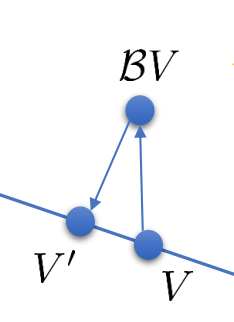
\includegraphics[scale=0.5]{figures/bellmanbackup.png}
    \caption{Bellman Backup Projection}
    \label{fig:bellmanbackup}
\end{figure}

Now we have the two operators defined, we can see that $\mathcal{B}$ is a contraction with respect to the l-$\infty$ norm, and the operator $\Pi$ is a contraction with respect to the l2 norm. But what if we impose one operator to another? Is the compound operator also a contraction? The answer is no. Therefore, such non-tabular Q-iterations do not have any convergence guarantee as the operator is not a contraction. 

What about fitted Q-iteration? Concisely, the fitted Q-iteration algorithm can be defined as $Q \leftarrow \Pi\mathcal{B}Q$. Therefore, the same reasoning can be applied to the fitted Q-learning: since the compound operator is no longer a contraction, we do not have any guarantee for convergence. We can say the same thing in online Q-iteration as well.

However, one might ask, in step 4 of Alg. \ref{alg:onlineQiter}, aren't we just doing gradient descent, which definitely converges? As a matter of fact, this is not real gradient descent in that the target value is constantly changing due to the off-policy nature of this algorithm. So we have this sad corollary: in general cases, fitted bootstrapped policy evaluation does not converge.
\chapter{Q-Function Methods}
Recall the algorithms that we discussed in last chapter: Alg. \ref{alg:fittedQ} and Alg. \ref{alg:onlineQiter}, where we devised a fitted Q-learning algorithm and a fully online version of it. We have also shown that Q-learning is fully off-policy, meaning that we do not care about the trajectory we are taking, we only care about the current transition and the next state we land in. So what is the problem with the above Q-learning algorithms? To see this, let us carefully look at step 4 of Alg. \ref{alg:onlineQiter}. The gradient step that we are taking is equivalently written as:
$$\phi\leftarrow \phi - \alpha\frac{dQ_\phi}{d\phi}(s_i,a_i)\left(Q_\phi(s_i,a_i) - \left[r(s_i,a_i)+\gamma\max_{a'}Q_\phi(s_i,a_i,s'_i,r_i)\right]\right)$$
This is not gradient descent! Because the ``target'' value $y_i$ is not constant and depends on our parameter $\phi$, and we are not taking gradient from $y_i$. Therefore, this is not the gradient descent step that we used to see before. Moreover, in step 2, we are only taking one sample of transition. This sampling scheme brings us two problems: the first one is that one sample is really hard to train the network (recall in online actor-critic, we would use parallel workers to obtain multiple online samples), and the second problem is the samples we are drawing are correlated in that the transitions are dependent on each other. As you may know, Stochastic Gradient Descent converges only if we are taking the correct gradient, and when the samples are IID. We violated both requirements, so the Q-learning algorithms in Alg. \ref{alg:fittedQ} and Alg. \ref{alg:onlineQiter} do not have any convergence guarantees. 

\section{Replay Buffers}
One of the solutions that we can implement to resolve the above correlation issue is to use a \textbf{replay buffer}. A replay buffer $\mathcal{B}$ is a buffer of transition data that contains the single samples that we have drawn so far. Therefore, in Q-learning, if we sample a batch from $\mathcal{B}$, the samples are no longer correlated, and we also keep updating the replay buffer by adding in real-world transitions. One can view this interaction in the image illustrated in Fig. \ref{fig:qwfb}.
\begin{figure}
    \centering
    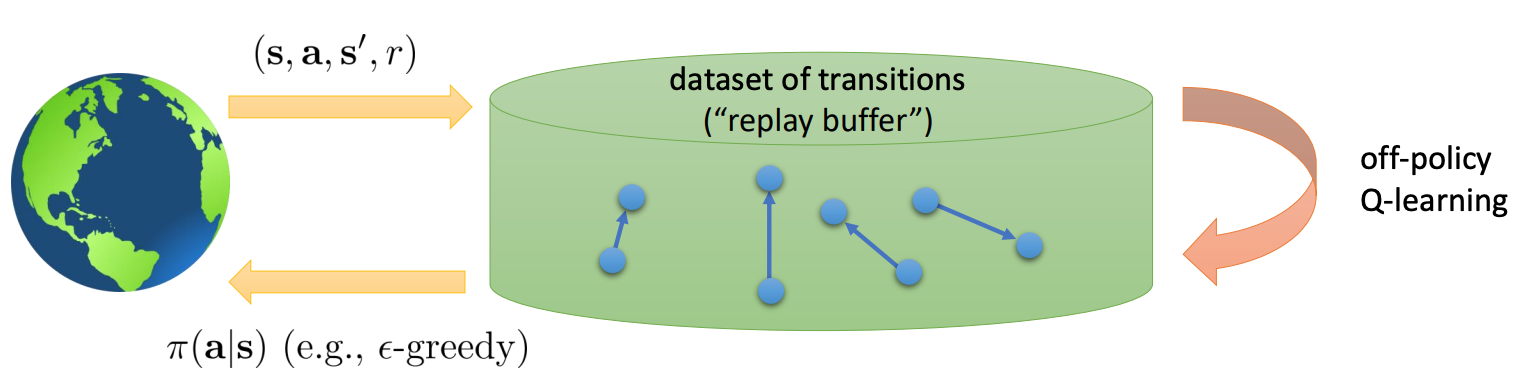
\includegraphics[scale=0.5]{figures/qwrb.png}
    \caption{Q-learning with replay buffers}
    \label{fig:qwfb}
\end{figure}


Putting it all together, we sketch out the full Q-learning algorithm with replay buffer in Alg. \ref{alg:QwRB}.
\begin{algorithm}[t!]
\caption{Q-Learning with Replay Buffer}
\begin{algorithmic}[1]
\label{alg:QwRB}
\REQUIRE Some base policy for data collection; hyperparameter $K$
\WHILE{true}
    \STATE Collect dataset $\{(s_i,a_i,s'_i,r_i)\}$ using some policy, add it to replay buffer $\mathcal{B}$
    \FOR{$K$ times}
        \STATE Sample a batch $(s_i,a_i,s'_i,r_i)$ from $\mathcal{B}$
        \STATE Set $y_i\leftarrow r(s_i,a_i) + \gamma \max_{a'_i}Q_\phi(s'_i,a'_i)$
        \STATE Set $\phi \leftarrow \phi-\alpha\Sigma_i\frac{dQ_\phi}{d\phi}(s_i,a_i)(Q_\phi(s_i,a_i) - y_i)$
    \ENDFOR
\ENDWHILE
\end{algorithmic}
\end{algorithm}
What have changed here in Alg. \ref{alg:QwRB} compared with Alg. \ref{alg:fittedQ}? In step 2, we are not only collecting dataset, but also adding the dataset to replay buffer $\mathcal{B}$. Inside the for loop, we are now sampling a batch of transitions from $\mathcal{B}$, which will bring us lower variance when we take the gradient step on the batch. We also periodically update $\mathcal{B}$.

The above solution solves the correlation problem, but we still need to address the wrong gradient problem. 

\section{Target Networks}
To solve the wrong gradient problem, we are essentially trying to solve the problem that the target value $y_i$ is heavily dependent on our gradient parameter $\phi$. Therefore, one way to improve this is to use a separate Q-function with another parameter $\phi'$ in order to decorrelate the two values. We should also use a well-defined $\phi'$, which can be set as the $\phi$ parameter 1000 steps ago. When setting $y_i$, we set it from the Q function with another parameter, thus decorrelating the two values. Together with the use of replay buffer, we alleviated the wrong policy and the correlation samples problems, as shown in Alg. \ref{alg:QwRB_tn}.
\begin{algorithm}[t!]
\caption{Q-Learning with Replay Buffer and Target Network}
\begin{algorithmic}[1]
\label{alg:QwRB_tn}
\REQUIRE Some base policy for data collection; hyperparameter $K$ and $N$
\WHILE{true}
\STATE Save target network parameters: $\phi' \leftarrow \phi$
\FOR{$N$ times}
    \STATE Collect dataset $\{(s_i,a_i,s'_i,r_i)\}$ using some policy, add it to replay buffer $\mathcal{B}$
    \FOR{$K$ times}
        \STATE Sample a batch $(s_i,a_i,s'_i,r_i)$ from $\mathcal{B}$
        \STATE Set $y_i\leftarrow r(s_i,a_i) + \gamma \max_{a'_i}Q_{\phi'}(s'_i,a'_i)$
        \STATE Set $\phi \leftarrow \phi-\alpha\Sigma_i\frac{dQ_\phi}{d\phi}(s_i,a_i)(Q_\phi(s_i,a_i) - y_i)$
    \ENDFOR
    \ENDFOR
\ENDWHILE
\end{algorithmic}
\end{algorithm}
Here we are frequently sampling batches from $\mathcal{B}$ and taking the gradient steps. We are less frequently updating the replay buffer as discussed in Alg. \ref{alg:QwRB}. We are even less frequently updating the network parameters, since we said one good choice for parameter $\phi'$ is to use $\phi$ 1000 steps ago.

Using target networks and replay buffers, we can sketch out a classic deep Q-learning algorithm (DQN), proposed by Minh et al. in \cite{mnih2013playing}. The pseudocode is in \ref{alg:dqn}. Here we choose $N$ to be a large number because our intention is to infrequently update the parameters. To further optimize the algorithm, it might feel weird abruptly update $\phi'$ after $N$ steps. Therefore, to alleviate this ``abruptness'', we can use \textbf{Polyak Averaging}: in step 6 of Alg. \ref{alg:dqn}, instead of copying $\phi$ every $N$ steps, we do $\phi' \leftarrow \tau\phi' + (1-\tau)\phi$. We also call such update a damped update.
\begin{algorithm}[t!]
\caption{Classic Deep Q-Learning Algorithm (DQN)}
\begin{algorithmic}[1]
\label{alg:dqn}
\WHILE{true}
    \STATE Take some action $a_i$ and observe $(s_i,a_i,s'_i,r_i)$ and add it to $\mathcal{B}$
    \STATE Sample mini-batch $\{s_j,a_j,s'_j,r_j\}$
    \STATE Compute $y_j = r_j + \gamma \max_{a'_j}Q_{\phi'}(s'_j,a'_j)$ using target network $Q_{\phi'}$
    \STATE $\phi \leftarrow \phi-\alpha\Sigma_j\frac{dQ_\phi}{d\phi}(s_j,a_j)(Q_\phi(s_j,a_j) - y_J)$
    \STATE update $\phi'$: copy $\phi$ every $N$ steps.
\ENDWHILE
\end{algorithmic}
\end{algorithm}

Now let us view the three different Q-learning algorithms in a more general way. As shown in Fig. \ref{fig:dqn}, there are three different steps in the algorithm. The first step is to collect data, the second step is to update the target in the target network, and the third step is to regress onto the Q-function. In the simplest, regression-based fitted Q-learning algorithm, process 3 is in the inner loop of process 2, which is in the inner loop of process 1. In online Q-learning, we evict the old transitions immediately, and process 1, 2, and 3 run at the same speed. In DQN, process 1 and 3 run at the same speed, but process 2 runs slower.
\begin{figure}
    \centering
    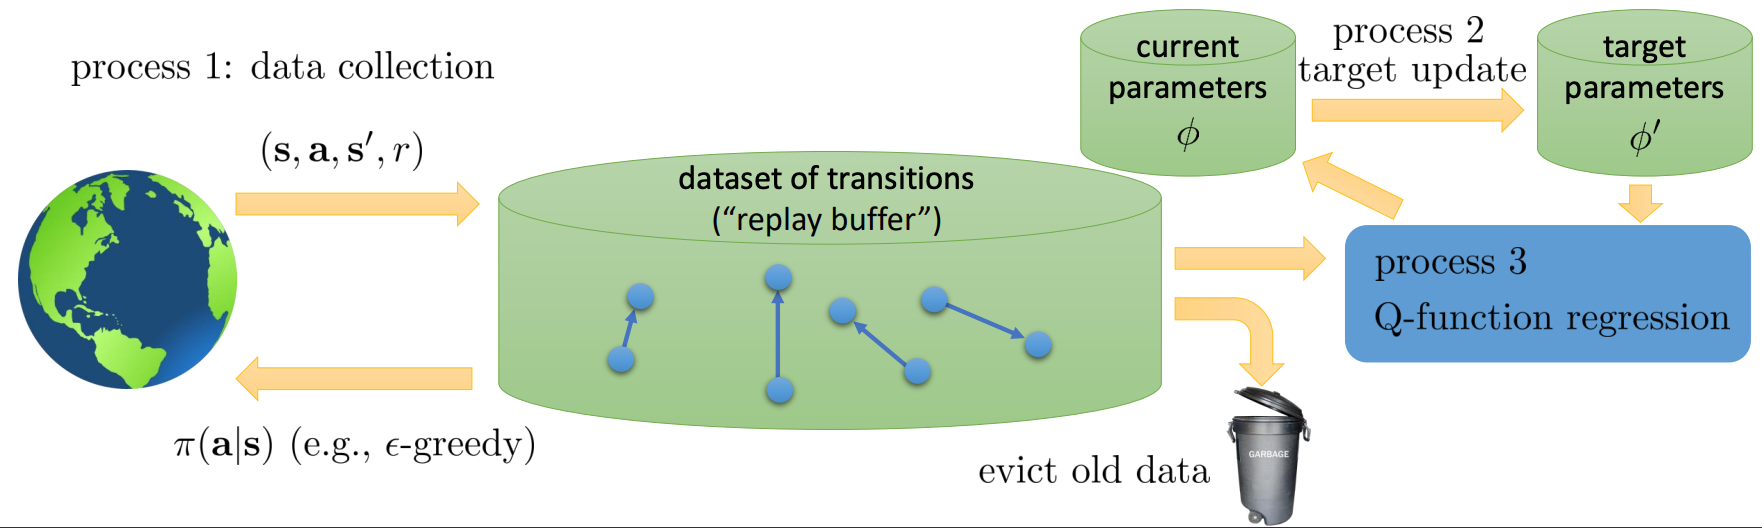
\includegraphics[scale=0.5]{figures/dqn.png}
    \caption{Q-learning in a more general view.}
    \label{fig:dqn}
\end{figure}

\section{Inaccuracy in Q-Learning}
Q-values are not necessarily accurate. The reason lies in the target value. Recall that the target value $y$ is defined as $y_j = r_j + \gamma \max_{a'_j}Q_{\phi'}(s'_j,a'_j)$. The $\max$ operation in the target is the main problem, because for two random variables $X_1$ and $X_2$, $\mathbb{E}[\max(X_1,X_2)] \geq \max(\mathbb{E}[X_1],\mathbb{E}[X_2])$. Therefore, when $Q_{\phi'}(s'_j,a'_j)$ is noisy, the max operation is going to overestimate the next Q-value.

\subsection{Double Q-Learning}
One might notice that $\max_{a'}Q_{\phi'}(s',a') = Q_{\phi'}(s',\argmaxA_{a'}Q_{\phi'}(s',a'))$. Thus, if we somehow managed to decorrelate the error from the selected action and the error from the Q-function, we could eliminate the erroneous overestimation. To achieve this, we can use two different networks to choose actions and evaluate the Q-function values. 
\begin{align*}
    Q_{\phi_A}(s,a) &\leftarrow r + \gamma Q_{\phi_B}\left(s',\argmaxA_{a'}Q_{\phi_A}(s',a')\right)\\
    Q_{\phi_B}(s,a) &\leftarrow r + \gamma Q_{\phi_A}\left(s',\argmaxA_{a'}Q_{\phi_B}(s',a')\right)
\end{align*}
Essentially we are using one network's parameter to update the value, while using the other's to select the action. Using the two separate networks, we are decorrelating the action selection and value evaluation errors, thus decreasing the overestimation in the Q-values.

In practice, we can just use the actual and target networks for the two separate networks. Therefore, instead of setting target $y$ as $y = r + \gamma Q_{\phi'}\left(s',\argmaxA_{a'}Q_{\phi'}(s',a')\right)$, we use the current network to select action, and use the target network to evaluate value: $y = r + \gamma Q_{\phi'}\left(s',\argmaxA_{a'}Q_{\phi}(s',a')\right)$.

\subsection{N-Step Return Estimator}
In the definition of our target $y$, $y_{i,t} = r_{i,t} + \max_{a_{i,t+1}}Q_{\phi'}(s_{i,t+1},a_{i,t+1})$, the Q-value only matters if it is a good estimate. If the Q-value estimate is bad, the only values that matter are from the reward term, so we are not learning much about the Q-function. To resolve this problem, let us recall the N-step cut trick we did in the actor-critic algorithm. In actor-critic algorithm, to leverage the bias and variance tradeoff in policy gradient, we can end the trajectory earlier, and only count the reward summed up to $N$ steps from now. Specifically, we can define the target as:
$$y_{i,t} = \sum_{t'=t}^{t+N-1}\gamma^{t-t'}r_{i,t} +\gamma^N \max_{a_{i,t+1}}Q_{\phi'}(s_{i,t+1},a_{i,t+1})$$
One subtle problem with this solution is that the learning process suddenly becomes on-policy, so we cannot efficiently make use of the off-policy data. Why is it on-policy? If we look at the summation of the rewards, we are collecting the rewards data using a certain trajectory, which is generated by a specific policy. Therefore, we end up having less biased target values when the Q-values are inaccurate, and in practice, it is faster in early stages of learning. However, it is only correct when we are learning on-policy. To fix this problem, one could ignore this mismatch, which somehow works very well in practice. Or one could cut the trace by dynamically adapting $N$ to get only on-policy data. Also, one could use importance sampling as we discussed before. For more details, please refer to this paper by Munos et al. \cite{munos2016safe}.
\subsection{Q-Learning with Continuous Actions}
Recall the implicit policy that we define using Q-learning:
\begin{align*}
\pi'(a_t|s_t) & = \begin{cases}
                1, & \mathrm{if } \;a_t = \argmaxA_{a_t}A^\pi(s_t,a_t)\\
                 0, & \mathrm{otherwise}
                    \end{cases}
\end{align*}
One problem with this definition is that the $\argmaxA$ operation cannot be easily applied if the actions are continuous. How are we going to address such an issue?

One option is to use various optimization techniques, as one may have seen in UC Berkeley's EE 127. Specifically, one could use SGD on the action space to produce an optimal $a_t$ by solving an optimization problem. Another simple approach is to stochastically optimize the Q-values by using some samples of the values from some pre-defined distribution (e.g. uniform): $\max_a Q(s,a) \simeq \max \{Q(s,a_1), ..., Q(s,a_N)\}$. One could also improve the accuracy by using some more sophisticated optimization techniques such as Cross-Entropy Method (CEM).

Option no. 2 is to use function classes that are easy to maximize. For example, one could use the Normalized Advantage Functions (NAF) proposed by Gu et al. in \cite{gu2016continuous}.

Another rather fancier option is to learn an approximate optimizer, which was originally proposed by Lillicrap et al. in \cite{lillicrap2015continuous}. The idea of Deep Deterministic Policy Gradient (which is actually a Q-learning in disguise) is to train another network $\mu_\theta(s)$ such that $\mu_\theta(s) \simeq \argmaxA_a Q_\phi(s,a)$. To train the network, one can see that the optimization of Q-function with respect to $\theta$ can be solved by $\theta \leftarrow \argmaxA_\theta Q_\phi(s,\mu_\theta(s))$ because by chain rule, $\frac{dQ_\phi}{d\theta} = \frac{da}{d\theta}\frac{dQ_\theta}{da}$. Then the new target becomes:
$$y_j = r_j + \muQ_{\phi'}(s'_j,\mu_\theta(s'_j))\simeq r_j + \muQ_{\phi'}(s'_j, \argmaxA_{a'}Q_{\phi'}(s'_j,a'_j))$$

The sketch of DDPG is in Alg. \ref{alg:ddpg}. In step 5, we are updating the Q-function, and in step 6, we are updating the argmax-er. Therefore, DDPG is essentially DQN with argmax-er.
\begin{algorithm}[t!]
\caption{Deep Deterministic Policy Gradient (DDPG)}
\begin{algorithmic}[1]
\label{alg:ddpg}
\WHILE{true}
    \STATE Take some action $a_i$ and observe $(s_i,a_i,s'_i,r_i)$ and add it to $\mathcal{B}$
    \STATE Sample mini-batch $\{s_j,a_j,s'_j,r_j\}$
    \STATE Compute $y_j = r_j + \gamma \max_{a'_j}Q_{\phi'}(s'_j,a'_j)$ using target networks $Q_{\phi'}$ and $\mu_{\theta'}$
    \STATE $\phi \leftarrow \phi-\alpha\Sigma_j\frac{dQ_\phi}{d\phi}(s_j,a_j)(Q_\phi(s_j,a_j) - y_J)$
    \STATE $\theta \leftarrow \theta + \beta\sum_j\frac{da}{d\theta}(s_j)\frac{dQ_\phi}{da}(s_j,a)$
    \STATE update $\phi'$ and $\theta'$
\ENDWHILE
\end{algorithmic}
\end{algorithm}



\chapter{Policy Gradients Theory}
Why does Policy Gradient algorithm work? Recall our generic policy gradient algorithm: we are essentially looping to constantly estimate the advantage function $\hat{A}^\pi(s_t,a_t)$ for the current policy $\pi$, and then we use this estimate to improve the policy by taking a gradient step on the policy parameter $\theta$, as shown in Alg. \ref{alg:reinforce}. This is very similar to the policy iteration algorithm that we discussed in last chapter; the idea of policy iteration is to constantly evaluate the advantage function $A^\pi(s,a)$ and update the policy accordingly using the $\argmaxA$ implicit policy. In this chapter, we are going to dive deeper into the policy gradient algorithm, and we will show that the policy gradient algorithm can be reduced to our policy iteration algorithm, which we will prove mathematically. 

\section{Policy Gradient as Policy Iteration}
The sum of rewards of RL was defined as $J(\theta) = \mathbb{E}_{\tau\sim p_\theta(\tau)}\left[\sum_t\gamma^tr(s_t,a_t)\right]$, which is an expectation taken under the trajectory distribution. We claim that given a new parameter $\theta'$, $J(\theta') - J(\theta) = \mathbb{E}_{\tau\sim p_{\theta'}(\tau)}\left[\sum_t\gamma^tA^{\pi_\theta}(s_t,a_t)\right]$, which is an expectation taken under the new policy's trajectory distribution. The difference of the two sums of rewards is the improvement of applying the new policy compared to using the old policy. We claim that this improvement is equal to the expected value of the old policy's advantage function value taken under the new policy's trajectory distribution. The proof is as follows:
\begin{align*}
    J(\theta') - J(\theta) &= J(\theta') - \mathbb{E}_{s_0\sim p(s_0)}\left[V^{\pi_\theta}(s_0)\right]\\
    &= J(\theta') - \mathbb{E}_{\tau\sim p_{\theta'}(\tau)}\left[V^{\pi_\theta}(s_0)\right]\\
    &= J(\theta') - \mathbb{E}_{\tau\sim p_{\theta'}(\tau)}\left[\sum_{t=0}^\infty\gamma^t V^{\pi_\theta}(s_t) - \sum_{t=1}^\infty\gamma^tV^{\pi_\theta}(s_t)\right]\\
    &= J(\theta') + \mathbb{E}_{\tau\sim p_{\theta'}(\tau)}\left[\sum_{t=0}^\infty\gamma^t\left(\gammaV^{\pi_\theta}(s_{t+1}) - V^{\pi_\theta}(s_t)\right)\right]\\
    &= \mathbb{E}_{\tau\sim p_{\theta'}(\tau)}\left[\sum_{t=0}^\infty\gamma^tr(s_t,a_t)\right] + \mathbb{E}_{\tau\sim p_{\theta'}(\tau)}\left[\sum_{t=0}^\infty\gamma^t\left(\gammaV^{\pi_\theta}(s_{t+1}) - V^{\pi_\theta}(s_t)\right)\right]\\
    &= \mathbb{E}_{\tau\sim p_{\theta'}(\tau)}\left[\sum_{t=0}^\infty\gamma^t\left(r(s_t,a_t) + \gamma V^{\pi_\theta}(s_{t+1})-V^{\pi_\theta}(s_t)\right)\right]\\
    &= \mathbb{E}_{\tau\sim p_{\theta'}(\tau)}\left[\sum_{t=0}^\infty\gamma^tA^{\pi_\theta}(s_t,a_t)\right]
\end{align*}
In the first two steps, we swapped out the initial states distribution in the expectation. This might seem weird at the first sight, but the intuition is that the initial state marginal is the same for any policy. Therefore, the expectation taken under the initial state marginal can be equivalently written as any policy's trajectory distribution, and for simplicity, we choose the policy of interest $\pi'$, with corresponding parameter $\theta'$.

Now we have proved our claim, but we see the result has a distribution mismatch: the expectation we take is under $\pi_{\theta'}$, but the advantage function $A$ is under $\pi_\theta$. It would be nice if we could make the two distributions the same. Therefore, we make use of our powerful statistical tool: \textbf{importance sampling}:

\begin{align*}
\mathbb{E}_{\tau\sim p_{\theta'}(\tau)}\left[\sum_{t=0}^\infty\gamma^tA^{\pi_\theta}(s_t,a_t)\right] &= \sum_t\mathbb{E}_{s_t\sim p_{\theta'}(s_t)}\left[\mathbb{E}_{a_t\sim \pi_{\theta'}(a_t|s_t)}\left[\gamma^t A^{\pi_\theta}(s_t,a_t)\right]\right]\\
&=\sum_t\mathbb{E}_{s_t\sim p_{\theta'}(s_t)}\left[\mathbb{E}_{a_t\sim \pi_{\theta}(a_t|s_t)}\left[\frac{\pi_{\theta'}(a_t|s_t)}{\pi_\theta(a_t|s_t)}\gamma^t A^{\pi_\theta}(s_t,a_t)\right]\right]
\end{align*}

Now the outer expectation is still under $\theta'$ state marginal. Can we simply ignore the distribution mismatch and say that it is approximately equal to $\sum_t\mathbb{E}_{s_t\sim p_{\theta}(s_t)}\left[\mathbb{E}_{a_t\sim \pi_{\theta}(a_t|s_t)}\left[\frac{\pi_{\theta'}(a_t|s_t)}{\pi_\theta(a_t|s_t)}\gamma^t A^{\pi_\theta}(s_t,a_t)\right]\right]$, which we define as $\bar{A}(\theta')$? We would be all set if the approximation holds, because if so, then $J(\theta') - J(\theta) \simeq \bar{A}(\theta')$, which means we can calculate $\nabla_{\theta'}\bar{A}(\theta')$ without generating new samples and calculating any new advantage functions because the only term that depends on $\theta'$ in $\bar{A}(\theta')$ is the policy term in the numerator of importance sampling ratio. Thus, we can just use the current samples from $\pi_\theta$.

\section{Distribution Mismatch Bound}
As we discussed above, if we could ignore the distribution mismatch, then we would solve a number of problems. So when can we indeed ignore the distribution mismatch? We claim that $p_\theta(s_t)$ is close to $p_{\theta'}(s_t)$ when $\pi_\theta$ is close $\pi_{\theta'}$. This claim sounds rather silly, but in light of this claim, we could quantify the mismatch and bound the distribution change.

\subsection{A Simple $\epsilon$ Bound}
First, let us assume that $\pi_\theta$ is deterministic, which means $a_t = \pi_\theta(s_t)$. Then as we have seen in imitation learning, $\pi_{\theta'}$ is close to $\pi_\theta$ if $\pi_{\theta'}(a_t\neq \pi_\theta(s_t)|s_t)\leq \epsilon$. Using the same probability bound we defined in imitation learning, we have the new policy's state marginal defined as:
$$p_{\theta'}(s_t) = (1-\epsilon)^tp_\theta(s_t) + (1-(1-\epsilon)^t)p_{mistake}(s_t)$$
and we can bound the prior distribution mismatch by using:
\begin{align*}
  |p_{\theta'}(s_t) - p_\theta(s_t)| &= (1-(1-\epsilon)^t)|p_{mistake}(s_t) - p_\theta(s_t)|\\
  &\leq 2(1-(1-\epsilon)^t)\\
  &\leq2\epsilon t
\end{align*}
This is not a good bound, but it is a bound.

Now let's focus on the more general case, that $\pi_\theta$ is am arbitrary distribution. Then we can try to quantify the notion of ``close'' by saying $\pi_\theta$ is close to $\pi_{\theta'}$ if:
$$|\pi_{\theta'}(a_t|s_t) - \pi_\theta(a_t|s_t)| \leq \epsilon \; \forall s_t$$
Here is a useful lemma that we will use later: if $|p_X(x) - p_Y(y)| = \epsilon$, then there exists a joint distribution of $x,y$, which we call $p(x,y)$ such that $p(x) = p_X(x)$ and $p(y) = p_Y(y)$ and $p(x=y) = 1-\epsilon$. Equivalently, this means that under these circumstances, $p_X(x)$ agrees with $p_Y(y)$ with probability $\epsilon$. If we plug in our $\pi_\theta$ and $\pi_{\theta'}$, then we can show that $\pi_{\theta'}(a_t|s_t)$ takes a different action than $\pi_\theta(a_t|s_t)$ with probability less than $\epsilon$. Using this lemma, we have the same bound as in the deterministic case:
\begin{align*}
  |p_{\theta'}(s_t) - p_\theta(s_t)| &= (1-(1-\epsilon)^t)|p_{mistake}(s_t) - p_\theta(s_t)|\\
  &\leq 2(1-(1-\epsilon)^t)\\
  &\leq2\epsilon t
\end{align*}
Now let us first focus on a more general case where we have a generic function of state $f(s_t)$:
\begin{align*}
    \mathbb{E}_{p_\theta'}(s_t)[f(s_t)] &= \sum_{s_t}p_{\theta'}(s_t)f(s_t)\\
    &\geq \sum_{s_t}p_\theta(s_t)f(s_t) - |p_\theta(s_t) - p_{\theta'}(s_t)|*\max_{s_t}f(s_t)\\
    &\geq \mathbb{E}_{p_\theta(s_t)}[f(s_t)] - 2\epsilon t\max_{s_t}f(s_t)
\end{align*}
Now, putting it all together, let us plug in the term inside the expectation taken under the mismatched distribution:
\begin{multline}
    \sum_t\mathbb{E}_{s_t\sim p_{\theta'}}(s_t)\left[\mathbb{E}_{a_t\sim \pi_\theta(a_t|s_t)}\left[\frac{\pi_{\theta'}(a_t|s_t)}{\pi_\theta(a_t|s_t)}\gamma^t A^{\pi_\theta}(s_t,a_t)\right]\right]\\
    \geq \sum_t\mathbb{E}_{s_t\sim p_{\theta}}(s_t)\left[\mathbb{E}_{a_t\sim \pi_\theta(a_t|s_t)}\left[\frac{\pi_{\theta'}(a_t|s_t)}{\pi_\theta(a_t|s_t)}\gamma^t A^{\pi_\theta}(s_t,a_t)\right]\right] - \sum_t 2\epsilon C
\end{multline}
where the constant term $C$ is a constant depending on the maximum reward, so in the finite horizon case, it should be of $O(Tr_{max})$, and in infinite horizon case, it should be of $O(r_{max}\gamma^t$, which can be simplified by convergence theory to $O(\frac{r_{max}}{1-\gamma})$ Therefore, for small $\epsilon$, we can simply ignore the mismatch. 

What have we proved? We have proved that we can update the policy parameter $\theta'$ by
$$\theta' \leftarrow \argmaxA_{\theta'} \sum_t \mathbb{E}_{s_t\sim p_{\theta}}(s_t)\left[\mathbb{E}_{a_t\sim \pi_\theta(a_t|s_t)}\left[\frac{\pi_{\theta'}(a_t|s_t)}{\pi_\theta(a_t|s_t)}\gamma^t A^{\pi_\theta}(s_t,a_t)\right]\right]$$
such that $|\pi_{\theta'}(a_t|s_t) - \pi_{\theta}(a_t|s_t)|\leq \epsilon$ if $\epsilon$ is small.

\subsection{A More Convenient Bound - KL Divergence}
We now use a better, more convenient bound, which is the KL-divergence. We claim that we can apply the aforementioned update if the total variational divergence is bounded by the KL-divergence as follows:
$$|\pi_{\theta'}(a_t|s_t) - \pi_{\theta}(a_t|s_t)|\leq \sqrt{\frac{1}{2}D_{KL}(\pi_{\theta'}(a_t|s_t)||\pi_{\theta}(a_t|s_t)}$$
where KL-divergence is defined as:
$$D_{KL}(p_1(x)||p_2(x)) = \mathbb{E}_{x\sim p_1(x)}\left[\log\frac{p_1(x)}{p_2(x)}\right]$$

Then the update rule of the policy parameter becomes:
$$\theta' \leftarrow \argmaxA_{\theta'} \sum_t \mathbb{E}_{s_t\sim p_{\theta}}(s_t)\left[\mathbb{E}_{a_t\sim \pi_\theta(a_t|s_t)}\left[\frac{\pi_{\theta'}(a_t|s_t)}{\pi_\theta(a_t|s_t)}\gamma^t A^{\pi_\theta}(s_t,a_t)\right]\right]$$
such that $D_{KL}(\pi_{\theta'}(a_t|s_t)||\pi_{\theta}(a_t|s_t))\leq \epsilon$. We have guaranteed improvement if we have small $\epsilon$.

\subsection{Enforcing the Distribution Mismatch Constraint}
Now how do we incorporate the constraint on the distribution mismatch with our objective? One way to do it is to introduce a Lagrangian because we have the following optimization problem:
\begin{equation}
\begin{aligned}
\theta'\leftarrow \argmaxA_{\theta'} \sum_t \mathbb{E}_{s_t\sim p_{\theta}}(s_t)\left[\mathbb{E}_{a_t\sim \pi_\theta(a_t|s_t)}\left[\frac{\pi_{\theta'}(a_t|s_t)}{\pi_\theta(a_t|s_t)}\gamma^t A^{\pi_\theta}(s_t,a_t)\right]\right]\\
\mathrm{s.t. }\;D_{KL}(\pi_{\theta'}(a_t|s_t)||\pi_{\theta}(a_t|s_t))\leq \epsilon
    \end{aligned}
\end{equation}
Then we can have our Lagrangian $\mathcal{L}(\theta', \lambda)$ as
$$\mathcal{L}(\theta', \lambda) = \sum_t \mathbb{E}_{s_t\sim p_{\theta}}(s_t)\left[\mathbb{E}_{a_t\sim \pi_\theta(a_t|s_t)}\left[\frac{\pi_{\theta'}(a_t|s_t)}{\pi_\theta(a_t|s_t)}\gamma^t A^{\pi_\theta}(s_t,a_t)\right]\right] - \lambda(D_{KL}(\pi_{\theta'}(a_t|s_t)||\pi_{\theta}(a_t|s_t)) - \epsilon)$$
Then we optimize in terms of the Lagrangian by first maximizing $\mathcal{L}(\theta', \lambda)$ with respect to $\theta'$, which we can just do incompletely for a few gradient steps, then we update the dual variable by $\lambda \leftarrow \lambda + \alpha(D_{KL}(\pi_{\theta'}(a_t|s_t)||\pi_{\theta}(a_t|s_t)) - \epsilon)$. This technique is an instance of dual gradient descent, and we will talk about it more in depth in a later chapter. Essentially, the intuition is that we raise $\lambda$ if the constraint is violated too much, and else lower it. 

\subsection{Other Optimization Techniques}
There are also some other ways to optimize based on the distribution mismatch bound. One way to do it is by using 1st order Taylor expansion. Since $\theta' \leftarrow \argmaxA_{\theta'}\bar{A}(\theta')$, we can apply first order Taylor expansion by
\begin{equation}
\begin{aligned}
\theta'\leftarrow \argmaxA_{\theta'} \nabla_{\theta}\bar{A}(\theta)(\theta'-\theta)\\
\mathrm{s.t. }\;D_{KL}(\pi_{\theta'}(a_t|s_t)||\pi_{\theta}(a_t|s_t))\leq \epsilon
    \end{aligned}
\end{equation}

From what we have learned in policy gradients, we can derive the gradient of $\bar{A}$ as follows:
$$\nabla_{\theta}\bar{A}(\theta) = \sum_t \mathbb{E}_{s_t\sim p_{\theta}}(s_t)\left[\mathbb{E}_{a_t\sim \pi_\theta(a_t|s_t)}\left[\frac{\pi_{\theta'}(a_t|s_t)}{\pi_\theta(a_t|s_t)}\gamma^t\nabla_{\theta'}\log\pi_{\theta'}(a_t|s_t) A^{\pi_\theta}(s_t,a_t)\right]\right]$$
and if we have $\pi_\theta \simeq \pi_{\theta'}$, then we can effectively cancel out the importance ratio:
$$\nabla_{\theta}\bar{A}(\theta) = \sum_t \mathbb{E}_{s_t\sim p_{\theta}}(s_t)\left[\mathbb{E}_{a_t\sim \pi_\theta(a_t|s_t)}\left[\gamma^t\nabla_{\theta'}\log\pi_{\theta'}(a_t|s_t) A^{\pi_\theta}(s_t,a_t)\right]\right] = \nabla_\theta J(\theta)$$
just like normal policy gradient.

Consequently, our original optimization problem can be equivalently written as:
\begin{equation}
\begin{aligned}
\theta'\leftarrow \argmaxA_{\theta'} \nabla_{\theta}J(\theta)^T(\theta'-\theta)\\
\mathrm{s.t. }\;D_{KL}(\pi_{\theta'}(a_t|s_t)||\pi_{\theta}(a_t|s_t))\leq \epsilon
    \end{aligned}
\end{equation}
We now have the RL objective in our optimization, then can we just use gradient ascent just like what we did in policy gradient? Well, it turns out gradient ascent is enforcing some other constraint:
\begin{equation}
\begin{aligned}
\theta'\leftarrow \argmaxA_{\theta'} \nabla_{\theta}J(\theta)^T(\theta'-\theta)\\
\mathrm{s.t. }\;\lvert|\theta'-\theta|\rvert^2\leq \epsilon
    \end{aligned}
\end{equation}
whose update rule can be written as $\theta' \leftarrow \theta + \sqrt{\frac{\epsilon}{\lvert|\nabla_\theta J(\theta)|\rvert^2}}\nabla_\theta J(\theta)$, and the square root term is just our learning rate, which depends on $\epsilon$.

Since the two optimization problems are not the same, we will tweak the KL-divergence constraint a little bit using Taylor expansion one more time. If the two policies are very similar to each other, one could approximate KL-divergence by $D_{KL}(\pi_(\theta')||\pi_\theta) \simeq \frac{1}{2}(\theta' - \theta)^TF(\theta'-\theta)$, where $F$ is called the Fisher-information matrix, and it is defined as $\mathbb{E}_{\pi_\theta}\usepackage{\left[\nabla_\theta\log \pi_\theta(a|s)\nabla_\theta\log\pi_\theta(a|s)^T\right]}$. This matrix $F$ can be estimated using samples, and it gives us a convenient quadratic bound. Using a technique similar to Newton-Raphson, we can update the parameter by $\theta' \leftarrow \theta  + \alpha F^{-1}\nabla_\theta J(\theta)$, and the learning rate $\alpha$ can be chosen as $\alpha = \sqrt{\frac{2\epsilon}{\nabla_\theta J(\theta)^TF\nabla_\theta}}$. Now our update rule is a lot more similar to gradient descent, except that in gradient descent, the l2 norm constrains the update step into a circle, while in our 2nd order approximation of KL-divergence, it constrains the update step into a ellipse. 

\chapter{Model-Based Reinforcement Learning}
What we have covered so far can be categorized as ``model-free'' reinforcement learning. The reason why it is called model-free is that the transition probabilities are unknown and we did not even attempt to learn the transition probabilities. Recall the RL objective:
\begin{align*}
  \pi_\theta(\tau) &= p_\theta(s_1,a_1,...,s_T,a_t)\\
  &= p(s_1)\prod_{t=1}^T\pi_\theta(a_t|s_t)p(s_{t+1}|s_t,a_t)\\
  \theta^* &= \argmaxA_\theta\mathbb{E}_{\tau\sim p_\theta(\tau)}\left[\sum_t r(s_t,a_t)\right]
\end{align*}
The transition probabilities $p(s_{t+1}|s_t,a_t)$ is not known in all the model-free RL algorithms that we have learned such as Q-learning and policy gradients. But what if we know the transition dynamics? Recall that at the very beginning of the notes we drew an analogy of RL and control theory; in many cases, we do know the system's internal transition. For example, in games, easily modeled systems, and simulated environments, the transitions are given to us. Moreover, it is not uncommon to learn the transition models: in classic robotics, system identification fits unknown parameters of a known model to learn how the system evolves, and one could also imagine a deep learning approach where we could potentially fit a general-purpose model to observed transition data for later use. In fact, the latter case is the essence of Model-based RL, where we learn the transition dynamics first, and then figure out how to choose actions. To learn about model-based RL, we shall start from a simpler case, where we know the transitions and determine how we control the system optimally based on the transitions. After this, we can apply our optimal control theory to the more general case, where we actually learn the transitions first.
\section{Optimal Control}
Optimal control is a task that we come across when we are well aware of the transition probabilities and we try to learn how to control the system optimally. In optimal control, there are two different categories of controller design: the first one is \textbf{open-loop} control, where we do not have any state feedbacks, and we roll out a sequence of actions based on the current state that we observe. The second one is called \textbf{closed-loop} control, where we determine the action at each time step based on the current state, and how we determine the action to apply is based on state feedbacks. In some cases, our transition functions are deterministic, while in others, the transition functions are stochastic.

In a open loop controller, if we have a deterministic transition in our system such that $a_{t+1} = f(s_t,a_t)$, then our action sequence should be determined by choosing those that can return the maximum rewards:
\begin{align*}
    a_1, ..., a_T&=\argmaxA_{a1...a_T}\sum_{t=1}^Tr(s_t,a_t)\\
    \mathrm{s.t. }\;a_{t+1} &= f(s_t,a_t)
\end{align*}
In stochastic scenarios, the transition function is a probabilistic distribution, where we have $p(s_{t+1}|s_t,a_t)$, and the action sequence should be chosen based on expectation of the rewards:
\begin{align*}
    p_\theta(s_1,...,s_T)&=p(s_1)\prod_{t=1}^Tp(s_{t+1}|s_t,a_t)\\
    a_1,...,a_T &= \argmaxA_{a_1,...,a_T}\mathbb{E}\left[\sum_t r(s_t,a_t)|a_1,...,a_T\right]
\end{align*}
Note that we roll out all actions to apply only based on the initial state marginal, so we do not consider any state-feedback in this case.

In a closed-loop controller, however, we keep interacting with the world, so we need a policy function that can tell us the action to apply if we input the current state: $a_t\sim \pi(a_t|s_t)$, which we call a state-feedback. We choose our policy function as follows:
\begin{align*}
    p(s_1,a_1,...,s_T,a_T) &= p(s_1)\prod_{t=1}^T\pi(a_t|s_t)p(s_{t+1}|s_t,a_t)\\
    \pi &=\argmaxA_\pi \mathbb{E}_{\tau\sim p(\tau)}\left[\sum_t r(s_t,a_t)\right]
\end{align*}
Generally, $\pi$ could take many forms, such as a neural net or time-variant linear controller $K_ts_t + k_t$.

\section{Open-loop Planning}
For now, let us focus on a simple, open-loop controller, and see how we choose actions using such controller. In open-loop scenarios, we roll out a sequence of actions by doing $\argmaxA$ on the sum of rewards:
$a_1,...,a_T = \argmaxA_{a_1,...,a_T}J(a_1,...,a_T)$
and compactly, we can say that $A = \argmaxA_A J(A)$.
\subsection{Random Shooting}
Perhaps the easiest and most intuitive stochastic optimization method in open-loop control is the random shooting method. In such method, we first sample some different action sequences $A_1,...,A_N$ from some known distribution (such as uniform), and then we choose $A_i$ based on $\argmaxA_i J(A_i)$. This is highly efficient in that we are not improving what we sample, so we might get stuck in some mediocre action sequence. Therefore, we can keep improving the samples we choose from a Gaussian distribution based on some elites sequences. This is the basic idea of Cross Entropy Method (CEM).

\subsection{Cross Entropy Method}
CEM improves upon the random shooting's guess and check scheme by choosing some elites sequences which give us higher rewards and refit the distribution to the high rewards. Intuitively, we are getting closer to higher rewards as we refit the distribution. Here is a sketch of CEM, as shown in Alg. \ref{alg:cem}.
\begin{algorithm}[t!]
\caption{Cross Entropy Method with Continuous-valued Input}
\begin{algorithmic}[1]
\label{alg:cem}
\REQUIRE Some base distribution for action sequence $p(A)$ 
\WHILE{true}
    \STATE Sample $A_1,...,A_N$ from $p(A)$
    \STATE Evaluate $J(A_1),...,J(A_N)$
    \STATE Pick elites $A_{i_1},...,A_{i_M}$ with the highest value, where $M<N$
    \STATE Refit $p(A)$ to elites $A_{i_1},...,A_{i_M}$
\ENDWHILE
\end{algorithmic}
\end{algorithm}
This algorithm is extremely simple and very fast if parallelized. However, it suffers from very harsh dimensionality limit and it only works for open-loop scenarios. 
\subsection{Monte Carlo Tree Search}
Now imagine our action space is discrete, we can apply a stochastic optimization technique called Monte Carlo Tree Search (MCTS), which is very popular in planning in stochastic games. The gist of this method is that in discrete action space, we are essentially expanding out a tree. However, the tree might be too big to expand out due to computational cost. Therefore, one way to save the computational cost is to partially expand the tree and use a policy to simulate a trajectory from the last expanded node. A generic sketch of MCTS is shown in Alg. \ref{alg:mcts}.
\begin{algorithm}[t!]
\caption{Generic Monte Carlo Tree Search (MCTS)}
\begin{algorithmic}[1]
\label{alg:mcts}
\REQUIRE Some base tree policy for expanding nodes, some base default policy to simulate a trajectory from a leaf
\WHILE{true}
    \STATE Find a leaf $s_l$ using TreePolicy($s_1$)
    \STATE Evaluate the leaf using DefaultPolicy($s_l$)
    \STATE Update all values in tree between $s_1$ and $s_l$
\ENDWHILE
Take best action from $s_1$
\end{algorithmic}
\end{algorithm}
Note that we the tree policy is not an actual policy, because it is just a method to traverse through our tree in order to select a node to expand. The default policy is an actual policy that is able to simulate the system. Since simulations are involved here, we have to be able to roll back to the original state.
\subsection{UCT Tree Policy}

In MCTS, how do we choose the nodes to expand? Intuitively, we need to keep choosing the nodes with high rewards so far, and simultaneously pick the ones that have not been chosen in order to explore. Therefore, one way to do it is to use the UCT tree policy. In this policy, we gauge the performance of each node by assigning a score function where Score$(s_t) = \frac{Q(s_t)}{N(s_t)}+2C\sqrt{\frac{2\ln{N(s_{t-1})}}{N(s_t)}}$. If the current node $s_t$ is not fully expanded, meaning that there is action that we never took before, then we choose new $a_t$; else, we choose the child with best Score($s_{t+1}$).

More details about MCTS can be found in \cite{browne2012survey} and \cite{guo2014deep}.

\subsection{Using Derivatives}
Let us consider the control theory counterpart of the RL objective. Essentially, we have a constrained optimization problem defined as follows:
$$\min_{u_1,...,u_T}\sum_{t=1}^Tc(x_t,u_t)\;\mathrm{s.t.}\;x_t = f(x_{t-1}, u_{t-1})$$
if we plug in the transition constraint, we have:
$$\min_{u_1,...,u_T}c(x_1,u_1) + c(f(x_1,u_1),u_2)+...+c(f(f(...)...),u_T)$$
which becomes an unconstrained optimization problem. Since it is unconstrained now, one might ask, can we do gradient descent on it? The usual answer is yes, but only if we use some more powerful optimization technique such as 2nd-order Newton method. Because optimization problems such as shooting methods are hard and often ill-conditioned via 1st order gradient descent. 
\subsection{Shooting Methods and Collocation Methods}
There are two different classes of gradient descent based method: shooting method and collocation method. In shooting methods, we optimize only on action sequences, so the actions are the only optimization variables. We only optimize upon the actions and apply the action to the state and see where it shoots to, so the states are the consequences of the actions that we optimize. The optimization problem can be written as:
$$\min_{u_1,...,u_T}c(x_1,u_1) + c(f(x_1,u_1),u_2)+...+c(f(f(...)...),u_T)$$

However, in collocation method, we optimize upon both actions and states, with constraints, and the optimization problem is written as:
$$\min_{u_1,...,u_T,x_1,...,x_T}\sum_{t=1}^Tc(x_t,u_t)\;\mathrm{s.t.}\;x_t = f(x_{t-1}, u_{t-1})$$

\subsection{Linear Quadratic Regulator (LQR)}
Let us start with a simple case of shooting method, where we apply a 2nd order-style optimization technique to achieve optimal control. The simple case assumes that we have a linear system, where the transition function is affine, and we have a quadratic cost function. 

Thus, the transition function should be of the form:
\[
f(x_t,u_t) = F_t \begin{bmatrix} x_t\\u_t\end{bmatrix}+f_t
\]
and the cost function should be of the form:
\[
c(x_t,u_t) = \frac{1}{2}\begin{bmatrix}x_t\\u_t\end{bmatrix}^TC_t\begin{bmatrix}x_t\\u_t\end{bmatrix}+\begin{bmatrix}x_t\\u_t\end{bmatrix}^Tc_t
\]
What we are doing right now is to solve for a closed-form solution for an optimal LQR controller. The idea is to use backward recursion. Since we are doing shooting method, we have $$\min_{u_1,...,u_T}c(x_1,u_1) + c(f(x_1,u_1),u_2)+...+c(f(f(...)...),u_T)$$
and the last item is the only term that depends on $u_T$. Therefore, as a base case, we can try to solve for $u_T$ first. In order to simplify our computation, let us define some blocks in the matrices that we defined above. Specifically, let us assume that
\[
C_T = \begin{bmatrix} C_{x_T,x_T}& C_{x_T,u_T}\\C_{u_t,x_T}&C_{u_T,u_T}\end{bmatrix}
\]
and
\[
c_T=\begin{bmatrix}c_{x_T}\\c_{u_T}\end{bmatrix}
\]

Since our cost function is
\[
Q(x_T,u_T) = \mathrm{const} + \frac{1}{2}\begin{bmatrix}x_T\\u_T\end{bmatrix}^TC_T\begin{bmatrix}x_T\\u_T\end{bmatrix}+\begin{bmatrix}x_T\\u_T\end{bmatrix}^Tc_T
\]
by setting gradient to 0, we will have 
\[
\nabla_{u_T}Q(x_T,u_T) = C_{u_t,x_T}x_T+C_{u_T,u_T}u_T+c_{u_T}^T=0
\]
By solving this equation, we have solved $u_T$, in terms of known constants and $x_T$:
\[
u_T = -C_{u_T,u_T}^{-1}(C_{u_t,x_T}x_T+c_{u_T})
\]
and to make notations more compact, let us denote $u_T$ as $u_T = K_Tx_T+k_T$, and $K_T = -C_{u_T,u_T}^{-1}C_{u_t,x_T}$, $k_T = -C_{u_T,u_T}^{-1}c_{u_T}$.

Now having solved our terminal control input $u_T$, which is fully determined by our terminal state $x_T$, we can eliminate $u_T$ in $Q(x_T,u_T).$ Plugging in, we have
\begin{align*}
V(x_T) &= \mathrm{const} + \frac{1}{2}\begin{bmatrix}x_T\\K_Tx_T+k_T\end{bmatrix}^TC_T\begin{bmatrix}x_T\\K_Tx_T+k_T\end{bmatrix}+\begin{bmatrix}x_T\\K_Tx_T+k_T\end{bmatrix}^Tc_T\\
&=\frac{1}{2}x_T^TC_{x_T,x_T}x_T + \frac{1}{2}x_T^TC_{x_T,u_T}K_Tx_T+ \frac{1}{2}x_T^TK_T^TC_{u_T,x_T}x_T + \frac{1}{2}x_T^TK_T^TC_{u_T,u_T}K_Tx_T\\& \phantomrel{=} {}  + x_T^TK_T^TC_{u_T,u_T}k_T + \frac{1}{2}x_T^TC_{x_T,u_T}k_T + x_T^Tc_{x_T} + x_T^TK_T^Tc_{u_T} + \mathrm{const}\\
&= \text{const} + \frac{1}{2}x_T^TV_Tx_T + x_T^Tv_T
\end{align*}
where we define $v_T$ and $V_T$ to make the notation more compact as follows:
\begin{align*}
    V_T &= C_{x_T,x_T} + C_{x_T,u_T}K_T +K_T^TC_{u_T,x_T} + K_T^TC_{u_T,u_T}K_T^T\\
    v_T&= c_{x_T} + C_{x_T,u_T}k_T+K_T^Tc_{u_T} + K_T^TC_{u_T,u_T}k_T
\end{align*}

Having solved the base case, we solve solve for other optimal control inputs backwards. Let us first proceed to solve for $u_{T-1}$ in terms of $x_{T-1}$. Now note that $u_{T-1}$ not only affects state $x_{T-1}$, but it also affects $x_T$ because of the system dynamics:
\[
f(x_{T-1}, u_{T-1}) = x_T = F_{T-1}\begin{bmatrix}x_{T-1}\\u_{T-1}\end{bmatrix} + f_{T-1}
\]
Therefore, the cost function from $T-1$ can be calculated as:
\[
Q(x_{T-1}, u_{T-1}) = \text{const} + \frac{1}{2}\begin{bmatrix}x_{T-1}\\u_{T-1}\end{bmatrix}^TC_{T-1}\begin{bmatrix}x_{T-1}\\u_{T-1}\end{bmatrix} + \begin{bmatrix}x_{T-1}\\u_{T-1}\end{bmatrix}^Tc_{T-1} + V(f(x_{T-1}, u_{T-1}))
\]
and if we plug the transition dynamics function into $V(x_T)$, we will have:
\[
V(x_T) = \text{const} + \frac{1}{2}\begin{bmatrix}x_{T-1}\\u_{T-1}\end{bmatrix}^TF_{T-1}^TV_TF_{T-1}\begin{bmatrix}x_{T-1}\\u_{T-1}\end{bmatrix} + \begin{bmatrix}x_{T-1}\\u_{T-1}\end{bmatrix}^TF_{T-1}^TV_Tf_{T-1}+\begin{bmatrix}x_{T-1}\\u_{T-1}\end{bmatrix}^TF_{T-1}^Tv_T
\]
More compactly, we write the cost function as:
\[
Q(x_{T-1}, u_{T-1}) = \text{const} +\frac{1}{2} \begin{bmatrix}x_{T-1}\\u_{T-1}\end{bmatrix}Q_{T-1}\begin{bmatrix}x_{T-1}\\u_{T-1}\end{bmatrix} + \begin{bmatrix}x_{T-1}\\u_{T-1}\end{bmatrix}^Tq_{T-1}
\]
where $Q_{T-1} = C_{T-1} + F^T_{T-1}V_TF_{T-1}$, and $q_{T-1} = c_{T-1} +  F^T_{T-1}V_Tf_{T-1} + F^T_{T-1}v_T$. To solve the optimization problem, we set the gradient to 0:
\[
\nabla_{u_{T-1}}Q(x_{T-1}, u_{T-1}) Q_{u_{T-1},x_{T-1}}x_{T-1} + Q_{u_{T-1},u_{T-1}}u_{T-1}+q_{u_{T-1}}^T=0
\]
solving the equation, we have the following expression for $u_{T-1}$:
\begin{align*}
    u_{T-1} &= K_{T-1}x_{T-1} + k_{T-1}\\
    K_{T-1} &= -Q^{-1}_{u_{T-1},u_{T-1}}Q_{u_{T-1},x_{T-1}}\\
    k_{T-1} &= -Q_{u_{T-1},u_{T-1}}q_{u_{T-1}}
\end{align*}

Applying the same technique backwards, we can solve for the states and inputs at each time step, as illustrated in Alg. \ref{alg:lqr}.
\begin{algorithm}[t!]
\caption{Solving for Linear Quadratic Regulator (LQR)}
\begin{algorithmic}[1]
\label{alg:lqr}
\STATE Backward Recursion
\FOR{$t = T$ to 1}
    \STATE $Q_t = C_t + F_t^TV_{t+1}F_t$
    \STATE $q_{t} = c_{t} +  F^T_{t}V_Tf_{t} + F^T_{t}v_{t+1}$
    \STATE $Q(x_{t}, u_{t}) = \text{const} +\frac{1}{2} \begin{bmatrix}x_{t}\\u_{t}\end{bmatrix}Q_{t}\begin{bmatrix}x_{t}\\u_{t}\end{bmatrix} + \begin{bmatrix}x_{t}\\u_{t}\end{bmatrix}^Tq_{t}$
    \STATE $u_t\leftarrow \argminA_{u_t}Q(x_t,u_t) = K_tx_t + k_t$
    \STATE $K_{t} &= -Q^{-1}_{u_{t},u_{t}}Q_{u_{t},x_{t}}$
    \STATE $k_{t} &= -Q_{u_{t},u_{t}}q_{u_{t}}$
    \STATE $V_t = Q_{x_t,x_t} + Q_{x_t,u_t}K_t + K^T_tQ_{u_t,x_t} + K_t^TQ_{u_t,u_t}K_t$
    \STATE $v_t = q_{x_t} + Q_{x_t,u_t}k_t + K_t^TQ_{u_t} + K^T_tQ_{u_t,u_t}k_t$
    \STATE $V(x_t) = \text{const} + \frac{1}{2}x_t^TV_tx_t + x_t^Tv_t$
\ENDFOR
\STATE Forward Recursion
\FOR{$t=1$ to T}
    \STATE $u_t = K_tx_t + k_t$
    \STATE $x_{t+1} = f(x_t,u_t)$
\ENDFOR
\end{algorithmic}
\end{algorithm}
In step 5 of Alg. \ref{alg:lqr}, Q-function represents the total cost from now until end if we take $u_t$ from state $x_t$, and in step 11, the V-function represents the total cost from now until end from state $x_t$, so $V(x_t) = \min_{u_t}Q_{x_t,u_t}$, which we call the cost-to-go function. 

What we have analyzed above is based on deterministic dynamics. What if the transition (dynamics) is stochastic? Specifically, consider the following setup:
\begin{align*}
    x_{t+1} &\sim p(x_{t+1}|x_t,u_t)\\
    p(x_{t+1}|x_t,u_t) &= \mathcal{N}\left(F_t\begin{bmatrix}x_t\\u_t\end{bmatrix} + f_t, \Sigma_t\right)
\end{align*}
where our transition is actually a Gaussian distribution with constant covariance. It turns out that we can apply the exact same algorithm, choosing actions according to $u_t = K_tx_t + k_t$, and we can ignore $\Sigma_t$ due to symmetry of Gaussians.

\subsection{Iterative LQR (iLQR)}
In LQR, we assumed that the dynamics are linear. In non-linear cases, however, we can apply a similar approach called iterative LQR. Specifically, we can iteratively apply Jacobian linearization to locally linearize the system with respect to an equilibrium point. Consequently, we approximate a non-linear system as a linear-quadratic system:
\begin{align*}
    f(x_t,u_t) &\simeq f(\hat{x_t}, \hat{u_t}) + \nabla_{x_t,u_t}f(\hat{x_t}, \hat{u_t})\begin{bmatrix}x_t-\hat{x_t}\\u_t-\hat{u_t}\end{bmatrix}\\
    c(x_t,u_t) &\simeq c(\hat{x_t}, \hat{u_t}) + \nabla_{x_t,u_t}c(\hat{x_t}, \hat{u_t})\begin{bmatrix}x_t-\hat{x_t}\\u_t-\hat{u_t}\end{bmatrix} + \frac{1}{2}\begin{bmatrix}x_t-\hat{x_t}\\u_t-\hat{u_t}\end{bmatrix}^T\nabla^2_{x_t,u_t}c(\hat{x_t}, \hat{u_t})\begin{bmatrix}x_t-\hat{x_t}\\u_t-\hat{u_t}\end{bmatrix}
\end{align*}

Now we have an LQR system with respect to the divergence from the action space and state space's equilibrium points:
\begin{align*}
    \Bar{f}(\delta x_t, \delta u_t) &= F_t \begin{bmatrix}\delta x_t\\\delta u_t\end{bmatrix}\\
    \Bar{c}(\delta x_t, \delta u_t) &= \frac{1}{2}\begin{bmatrix}\delta x_t\\\delta u_t\end{bmatrix}^TC_t\begin{bmatrix}\delta x_t\\\delta u_t\end{bmatrix}^Tc_t
\end{align*}
where 
\begin{align*}
    F_t &= \nabla_{x_t,u_t}f(\delta x_t, \delta u_t) \\
    C_t &= \nabla^2_{x_t,u_t}c(\delta x_t, \delta u_t)\\
    c_t &= \nabla_{x_t,u_t}c(\delta x_t, \delta u_t)
\end{align*}
Then we can iteratively run LQR with dynamics $\Bar{f}$, cost $\Bar{c}$, state $\delta x_t$, and action $\delta u_t$.
\begin{algorithm}[t!]
\caption{Iterative LQR (iLQR)}
\begin{algorithmic}[1]
\label{alg:ilqr}
\WHILE{until convergence}
    \STATE $F_t = \nabla_{x_t,u_t}f(\delta x_t, \delta u_t)$
    \STATE $C_t = \nabla^2_{x_t,u_t}c(\delta x_t, \delta u_t)$
    \STATE $c_t = \nabla_{x_t,u_t}c(\delta x_t, \delta u_t)$
    \STATE Run LQR backward recursion on state $\delta x_t = x_t - \hat{x_t}$ and action $\delta u_t = u_t - \hat{u_t}$
    \STATE Run forward pass with real nonlinear dynamics and $u_t = K_t(x_t-\hat{x_t}) + k_t + \hat{u_t}$
    \STATE Update $\hat{x_t}$ and $\hat{u_t}$ based on states and actions in forward pass
    \ENDWHILE
\end{algorithmic}
\end{algorithm}


A sketch of iLQR is shown in Alg. \ref{alg:ilqr}. In essence, iLQR is an approximation of Newton's method for solving $\min_{u_1,...,u_T}c(x_1,u_1) + c(f(x_1,u_1),u_2)+...+c(f(f(...)...),u_T)$.

\section{Model-based RL}
In this section, we are going to cover a rather simpler case of model-based RL. Specifically, we are going to talk about a technique to learn a model of the system first, and then use the optimal control technique we covered last time to improve the model. Furthermore, we will learn to address uncertainty in the model such as model mismatch and imperfection.
\subsection{Basics}
Why do we learn the model? Because when the model is unknown, we can learn the model so that we know $f(s_t,a_t) = s_{t+1}$ or $p(s_{t+1}|s_t,a|t)$ in stochastic case, we could use the tools from optimal control to maximize our rewards. 

Our first attempt is naive, we learn $f(s_t,a_t)$ from data, and then plan through it. We call this approach model-based RL version 0.5, or vanilla model-based RL, as shown in algorithm \ref{alg:mb05}.
\begin{algorithm}[t!]
\caption{Model-based Reinforcement Learning Version 0.5}
\begin{algorithmic}[1]
\label{alg:mb05}
\REQUIRE Some base policy for data collection $\pi_0$
\STATE Run base policy $\pi(a_t|s_t)$ (e.g. random policy) to collect $\mathcal{D} = \{(s,a,s')_i\}$
\STATE Learn dynamics model $f(s,a)$ to minimize $\sum_i\lvert|f(s_i,a_i)-s'_i|\rvert^2$
\STATE Plan through $f(s,a)$ to choose actions
\end{algorithmic}
\end{algorithm}
This is essentially what people do in system identification, which is a technique used in classic robotics, and it is effective when we can hand-engineer a dynamics representation using our knowledge of physics, and fit just a few parameters. However, it does not work generally because of distribution mismatch: when the model is imperfect, we might suffer from false learning. Furthermore, since we are blindly following a trajectory, the mismatch exacerbates as we use more expressive model classes, when $p_{\pi_0}(s_t)\neq p_{\pi_f}(s_t)$.

Acknowledging this disadvantage, we could improve the vanilla model-based RL by making $p_{\pi_0}(s_t) = p_{\pi_f}(s_t)$. As we have seen in Alg. \ref{alg:dagger}, we can keep aggregating data into our dataset in order to make our model converge to demonstration model. Applying the same approach, we keep updating the dataset by running the current model, and then update the model accordingly. Take a look at the updated model-based RL algorithm in Alg. \ref{alg:mb10}.
\begin{algorithm}[t!]
\caption{Model-based Reinforcement Learning Version 1.0}
\begin{algorithmic}[1]
\label{alg:mb10}
\REQUIRE Some base policy for data collection $\pi_0$
\STATE Run base policy $\pi(a_t|s_t)$ (e.g. random policy) to collect $\mathcal{D} = \{(s,a,s')_i\}$
\WHILE{True}
\STATE Learn dynamics model $f(s,a)$ to minimize $\sum_i\lvert|f(s_i,a_i)-s'_i|\rvert^2$
\STATE Plan through $f(s,a)$ to choose actions
\STATE Execute those actions and add the resulting data $\{(s,a,s')_j\}$ to $\mathcal{D}$
\ENDWHILE
\end{algorithmic}
\end{algorithm}
Version 1.0 addresses the model mismatch issue and drives the current model as close as possible to the true dynamics model. However, we are still blindly following a trajectory in step 5 of Alg. \ref{alg:mb10}, and if we made a mistake, we would follow the wrong step which makes the mistake exacerbate. Therefore, we need to somehow adjust our plan as time goes on. One way to do this is to borrow some ideas from modern control theory: Model Predictive Control (MPC).

In MPC, we are given the system's dynamics model, and we are trying to design an adaptive controller by solving a finite time constrained optimal control problem at each time step, and take only the first action in the generated sequence of actions. Then we replan based on the new state. For sake of simplicity, we will skip the discussion about safe set and terminal set in MPC in this chapter. But the ``replan'' idea in MPC is exactly what we need to improve our model-based RL version 1.0. We essentially are aiming to take one action in the planned sequence and only observe one new state, and then append the observed transition to our dataset $\mathcal{D}$. The improvement is shown in Alg. \ref{alg:mb15}.
\begin{algorithm}[t!]
\caption{Model-based Reinforcement Learning Version 1.5}
\begin{algorithmic}[1]
\label{alg:mb15}
\REQUIRE Some base policy for data collection $\pi_0$, hyperparameter $N$
\STATE Run base policy $\pi(a_t|s_t)$ (e.g. random policy) to collect $\mathcal{D} = \{(s,a,s')_i\}$
\FOR{every $N$ steps}
\WHILE{True}
\STATE Learn dynamics model $f(s,a)$ to minimize $\sum_i\lvert|f(s_i,a_i)-s'_i|\rvert^2$
\STATE Plan through $f(s,a)$ to choose actions
\STATE Execute the first planned action, observe resulting state $s'$ (MPC)
\STATE Append $(s,a,s')$ to dataset $\mathcal{D}$
\ENDWHILE
\ENDFOR
\end{algorithmic}
\end{algorithm}
The while loop in algorithm \ref{alg:mb15} refers to replanning in MPC, which is solving for an optimization problem at each time step after we take the first action planned. The for loop, however, means that we are periodically retraining the model in order to make it closer to the true underlying transition model. Intuitively, the more frequently the agent replans, the less perfect each individual plan needs to be, because since we are frequently replanning, we are able to correct our mistakes made in previous plans more easily. Consequently, one is able to correct the plans as one increase the replanning frequency. Therefore, if we are frequently replanning, we could use shorter horizons in the CFTOC problem that MPC is solving. 

\subsection{Performance Gaps in Model-based RL}
Believe it or not, sometimes model-based RL performs worse than model-free RL. The problem is from step 5 of algorithm \ref{alg:mb15}. In this step, we plan through the model to choose actions, which means we are solving an optimization problem based on the data we collect. One could imagine that if we overfit the data, the agent might have some wrong belief about the model, thus generating wrong actions. Pictorially, this phenomenon is illustrated in Fig. \ref{fig:overfit}.
\begin{figure}
    \centering
    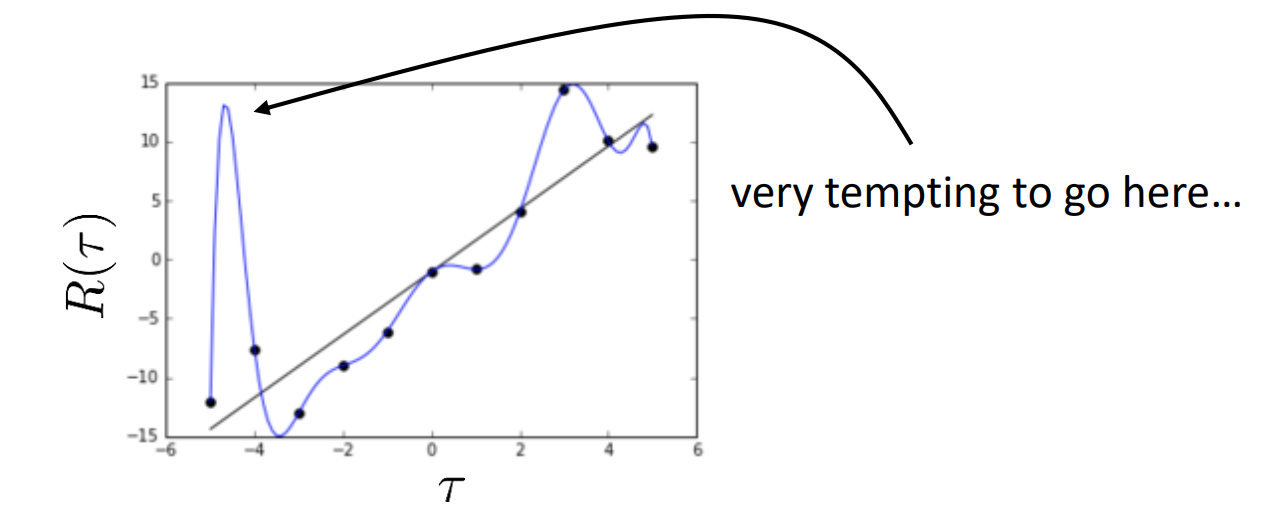
\includegraphics[scale=0.5]{figures/overfit.png}
    \caption{False belief about the model from overfitting}
    \label{fig:overfit}
\end{figure}

Therefore, we need to explore to get better, more representative data of the model, thus preventing overfitting and false belief. The expected value of the reward is not the same as optimistic or pessimistic. In step 5, when we choose actions, we only take actions for which we think we will get high reward in expectation, with respect to uncertain dynamics, which avoids exploiting the model too much.

\subsection{Uncertainty-aware Models}
Under imperfect models and model mismatch, one might expect wrong actions planned. Therefore, one way to deal with this problem is to construct an uncertainty-aware model, where we can quantitatively estimate the uncertainty in the model, so that we can assess the accuracy of the model and the planned actions. 

The first idea is to use entropy of output distribution, and as we know, higher entropy means higher uncertainty. We can estimate the entropy of $p(s_{t+1}|s_t,a_t)$. However, this is not enough because when the model is wrong, we might still have low variance, thus low entropy. Even though in some regions the model is highly uncertain, the output entropy is still low.

The reason why entropy of the output distribution alone is not expressive enough is that there are two types of uncertainty:
\begin{itemize}
    \item aleatoric (statistical) uncertainty, where the data itself is noisy.
    \item epistemic (model) uncertainty, where the model is certain about data, but we are not certain about model.
\end{itemize}
These two types of uncertainty are not the same. We cannot gauge the correctness of the second model based on the output entropy, and the entropy of the first model might be higher even though it is potentially a very ``good'' model. 

The second idea is to estimate the model uncertainty, where we essentially estimate how uncertainty we are about the model.
\begin{figure}
    \centering
    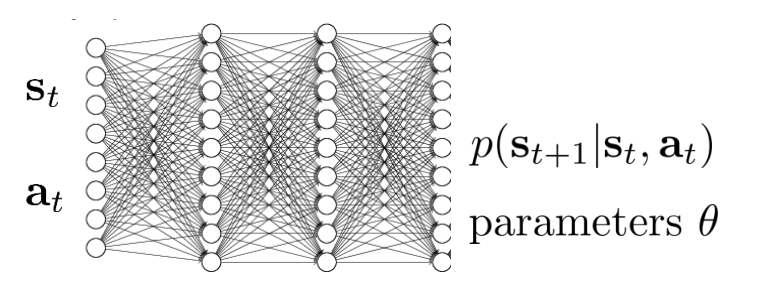
\includegraphics[scale=0.5]{figures/modelnn.png}
    \caption{Estimating the model using a neural net}
    \label{fig:modelnn}
\end{figure}
Usually, we use maximum likelihood estimation, where
\[
\argmaxA_\theta \log p(\theta|\mathcal{D}) = \argmaxA_\theta \log p(\mathcal{D}|\theta)
\]
Instead if we estimate the posterior of data $p(\theta|\mathcal{D})$ instead of argmax, the entropy of the distribution gives us the model uncertainty from the data. Moreover, we can predict using $\int p(s_{t+1}|s_t,a_t,\theta)p(\theta|\mathcal{D}) d\theta$.

To learn the posterior distribution, we can apply bootstrap ensembles, where we use multiple networks to learn the same distribution. Formally, say we have $N$ networks, each with a parameter $\theta_i$ to learn $p(s_{t+1}|s_t,a_t)$, we can then estimate the posterior by:
\[
p(\theta|\mathcal{D}) \simeq \frac{1}{N}\sum_i \delta(\theta_i)
\]
where $\delta(\cdot)$ is the direc-delta function. To train it, we need to generate independent datasets to get independent models. One way to do this is to train $\theta_i$ on $\mathcal{D}_i$ sampled with replacement from $\mathcal{D}$. This method is simple, but it is a very crude approximation. 

With this ensemble of networks, we choose actions a little differently. Before, we choose actions by $J(a_1,\dots,a_H) = \sum_{t=1}^Hr(s_t,a_t)$, where $s_{t+1} = f(s_t,a_t)$, and now we average over the ensemble by $J(a_1,\dots,a_H) = \frac{1}{N}\sum_{i=1}^N\sum_{t=1}^Hr(s_{t,i},a_{t,i})$, where $s_{t+1,i} = f(s_{t,i},a_{t,i})$

In general, for candidate action sequence $a_1,\dots,a_H$, we first sample $\theta \sim p(\theta|\mathcal{D})$, then at each time step $t$, we sample $s_{t+1}\sim p(s_{t+1}|s_t,a_t,\theta)$, then we calculate the reward $R = \sum_t r(s_t,a_t)$, and we repeat the aforementioned steps and accumulate the average reward.
% idk how this works....
\subsection{Latent Space Model}
In many cases, we are given very complex observations of the states such as pixel-based images, where we do not have full access to the states. To learn the dynamics using observations, we need to learn from the latent space and infer the states from observations. 
\begin{figure}
    \centering
    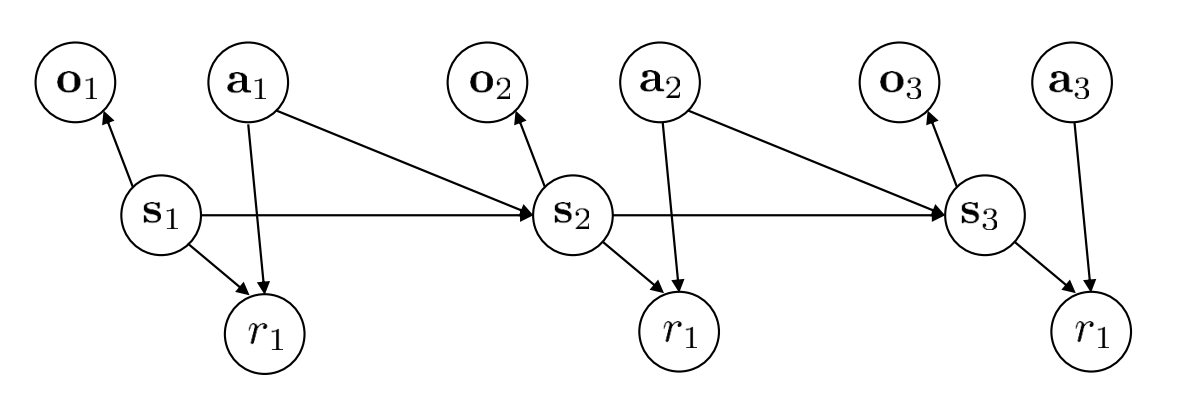
\includegraphics[scale=0.4]{figures/latent.png}
    \caption{Latent space model}
    \label{fig:latent}
\end{figure}
From Fig. \ref{fig:latent}, we can see that we need to learn the following models:
\begin{itemize}
    \item $p(o_t|s_t)$, the observation model
    \item $p(s_{t+1}|s_t,a_t)$, the dynamics model
    \item $p(r_t|s_t,a_t)$, the reward model
\end{itemize}

Recall that in high level, model-based RL algorithms are basically doing a maximum likelihood estimation in training given fully observed states:
\[
\max_\phi \frac{1}{N}\sum_{i=1}^N\sum_{t=1}^T\log p_\phi(s_{t+1,i}|s_{t,i},a_{t,i})
\]
then with latent models, we are not sure about the actual state, so we take the expected value:
\[
\max_\phi \frac{1}{N}\sum_{i=1}^N\sum_{t=1}^T\mathbb{E}\left[\log p_\phi(s_{t+1,i}|s_{t,i},a_{t,i}) + \log p_\phi(o_{t,i}|s_{t,i})\right]
\]
where the expectation is with respect to the distribution of $(s_t,s_{t+1})\sim p(s_t,s_{t+1}|o_{1:T},a_{1:T})$

However, the posterior distribution $p(s_t,s_{t+1}|o_{1:T},a_{1:T})$ is usually intractable if we have very complex dynamics. As a result, we could instead try to learn an approximate posterior, which we call $q_\psi(s_t|o_{1:t},a_{1;t})$. We could also learn $q_\psi(s_t,s_{t+1}|o_{1:t},a_{1;t})$ and $q_\psi(s_t|o_t)$. We call this technique learning an \textbf{encoder}. Learning the distribution $q_\psi(s_t|o_t)$ is crude, but it is the simplest to implement. If we just decide to learn this distribution for now, then the expectation becomes:
\[
\max_\phi \frac{1}{N}\sum_{i=1}^N\sum_{t=1}^T\mathbb{E}\left[\log p_\phi(s_{t+1,i}|s_{t,i},a_{t,i}) + \log p_\phi(o_{t,i}|s_{t,i})\right]
\]
such that the expectation is with respect to $s_t\sim q_\psi(s_t|o_t)$, $s_{t+1}\sim q_\psi(s_{t+1}|o_{t+1})$

For now, let us focus on a simple case where $q(s_t|o_t)$ is deterministic, because the stochastic requires variational inference, which will be covered in-depth in a later chapter. In deterministic case, we are training a neural net $g_\psi(o_t) = s_t$ using a direc-delta function such that $q_\psi(s_t|o_t) = \delta(s_t = g_\psi(o_t))$. Then the expectation can be simplified as
\[
\max_\phi \frac{1}{N}\sum_{i=1}^N\sum_{t=1}^T\log p_\phi(g_\psi(o_{t+1,i})|g_\psi(o_{t,i}),a_{t,i}) + \log p_\phi(o_{t,i}|g_\psi(o_{t,i}))
\]
Now everything is differentiable, we can train using backpropagation. 

Thus, we can slightly modify Alg. \ref{alg:mb15} so that we can deal with observations and latent space. We show the sketch of this slightly modified algorithm in Alg. \ref{alg:mblatent}. In step 4, we are respectively learning the dynamics, reward model, observation model, and encoder.
\begin{algorithm}[t!]
\caption{Model-based Reinforcement Learning with Latent States}
\begin{algorithmic}[1]
\label{alg:mblatent}
\REQUIRE Some base policy for data collection $\pi_0$, hyperparameter $N$
\STATE Run base policy $\pi(a_t|s_t)$ (e.g. random policy) to collect $\mathcal{D} = \{(s,a,s')_i\}$
\FOR{every $N$ steps}
\WHILE{True}
\STATE Learn dynamics model $p_\phi(s_{t+1}|s_t,a_t),p_\phi(r_t|s_t),p(o_t|s_t),g_\psi(o_t)$
\STATE Plan through $f(s,a)$ to choose actions
\STATE Execute the first planned action, observe resulting state $o'$ (MPC)
\STATE Append $(o,a,o')$ to dataset $\mathcal{D}$
\ENDWHILE
\ENDFOR
\end{algorithmic}
\end{algorithm}

Interested readers can refer to \cite{watter2015embed} and \cite{zhang2018solar} for more information on learning from pixel-based images as latent states.
\chapter{Model-based Policy Learning}
So far we have covered the basics of model-based RL that we first learn a model and use a model for control. We have seen that this approach does not work well in general because of the effect of distributional shift in model-based RL. We have also seen the method to quantify uncertainty in our model in order to alleviate this issue. The methods we covered so far do not involve learning policies. In this chapter, we will cover model-based reinforcement learning of policies. Specifically, we will learn global policies and local policies, and combine local policies into global policies using guided policy search and policy distillation. We shall understand how and why we should use models to learn policies, global and local policy learning, and how local policies can be merged via supervised learning into a global policy.

We have seen the difference between a closed-loop and open-loop controller. We also discussed why an open-loop controller is suboptimal because we are rolling out a whole sequence of actions solely based on one state observation. Therefore, it would be more ideal if we could design a closed-loop controller where state feedbacks can help us correct the mistakes we make. Recall in a stochastic environment, we are optimizing over the policy as follows:
\begin{align*}
    p(s_1,a_1,\dots,s_T,a_T)&=p(s_1)\prod_{t=1}^T\pi(a_t|s_t)p(s_{t+1}|s_t,a_t)\\
    \pi&=\argmaxA_\pi \mathbb{E}_{\tau\sim p(\tau)}\left[\sum_t r(s_t,a_t)\right]
\end{align*}
and $\pi$ could take several forms: $\pi$ can be a neural net, which we call a \textbf{global} policy, and it can also be a time-varying linear controller $K_t s_t + k_t$ as we saw in LQR, which we call a \textbf{local} policy.

\section{Back-propagate into the Policy}
Let us start with a simple solution for model-based policy learning. Ideally, we could build a computational graph in Tensorflow, and calculate the partial derivatives step by step so that we can backpropage into policy and optimize the policy, illustrated in Fig. \ref{fig:poliback}.
\begin{figure}
    \centering
    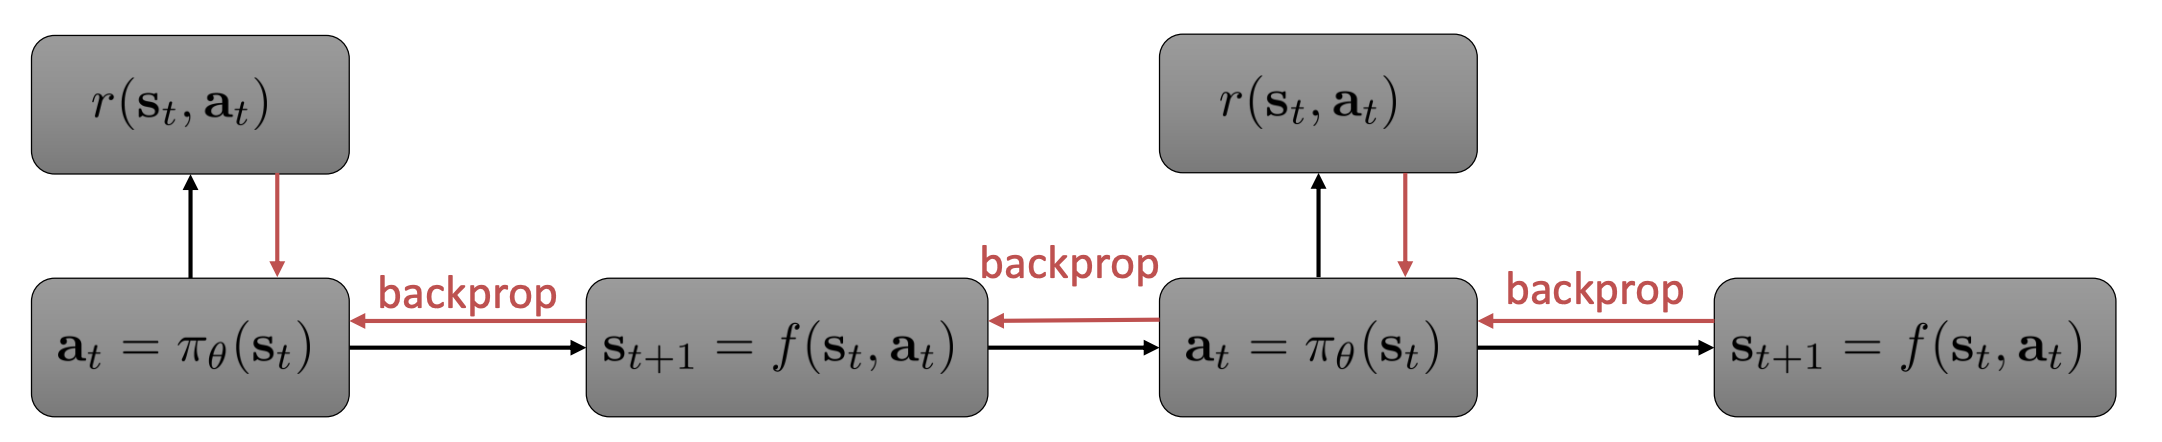
\includegraphics[scale=0.4]{figures/poliback.png}
    \caption{Back-propagate into policies}
    \label{fig:poliback}
\end{figure}
Then we can modify our model-based policy-free RL algorithm to accomodate this new policy learning process in Alg. \ref{alg:mb20}.
\begin{algorithm}[t!]
\caption{Model-based Reinforcement Learning Version 1.5}
\begin{algorithmic}[1]
\label{alg:mb20}
\REQUIRE Some base policy for data collection $\pi_0$
\STATE Run base policy $\pi_0(a_t|s_t)$ (e.g. random policy) to collect $\mathcal{D} = \{(s,a,s')_i\}$
\WHILE{True}
\STATE Learn dynamics model $f(s,a)$ to minimize $\sum_i\lvert|f(s_i,a_i)-s'_i|\rvert^2$
\STATE Backpropagate through $f(s,a)$ into the policy to optimize $\pi_\theta(a_t|s_t)$
\STATE Run $\pi_\theta(a_t|s_t)$, appending the visited tuples $(s,a,s')$ to $\mathcal{D}$.
\ENDWHILE
\end{algorithmic}
\end{algorithm}
\subsection{Vanishing and Exploding Gradients}
One problem with Alg. \ref{alg:mb20}, or general gradient-based optimization is that as we progress into the time steps, we might encounter vanishing or exploding gradients. Because as we apply chain rule, the gradients get multiplied by each other, so we the product may get extremely big (exploding) or extremely small (vanishing), making optimization a lot harder. Furthermore, we have similar parameter sensitivity problems as shooting methods, but we no longer have convenient second order LQR-like method, because the policy function is extremely complicated and policy parameters couple all the time steps, so no dynamic programming. % what does this mean

So what can we do about it? First, we can use model-free RL algorithms with synthetic samples generated by the model. Essentially, we are using models to accelerate model-free RL. Second, we cam use simpler policies than neural nets such as LQR, and train local policies to solve simple tasks, and then combine them into global policies via supervised learning. 

\section{Model-free Optimization with a Model}
Recall the equation from policy gradients:
\[
\nabla_\theta J(\theta) \simeq \frac{1}{N}\sum_{i=1}^N\sum_{t=1}^T\nabla_\theta \log\pi_\theta(a_{i,t}|s_{i,t})\hat{Q}^\pi_{i,t}
\]
Note that we are not doing any backprop through time in policy gradient because we are calculating the gradient with respect to an expectation, so we can just take the derivative of the probability of the samples instead of the actual dynamics function. 

Then we look at the regular backprop (pathwise) gradient, we see a more chain rule-like gradient:
\[
\nabla_\theta J(\theta) = \sum_{t=1}^T\frac{dr_t}{ds_t}\prod_{t'=2}^t\frac{d{s_{t'}}}{da_{t'-1}}\frac{da_{t'-1}}{ds_{t'-1}}
\]
The two gradients are different, because the policy gradient is for stochastic systems while the backprop policy is for deterministic systems. But using variational inference, we can prove that they are calculating the same gradient differently, this having different tradeoffs. We will talk about variational inference more in-depth in the next chapter. 

Actually, given more samples to reduce variance, policy gradient is more stable because it does not require multiplying many Jacobians. However, if our models are inaccurate, the samples we use from the wrong model will be incorrect, and the mistakes are likely to exacerbate as time goes on. So it would be nice to use such model-free optimizer and keep the rolled out samples' trajectory short. This is essentially what Dyna algorithm does.

\subsection{Dyna}
Dyna is an online Q-learning algorithm that performs model-free RL with a model. 
\begin{algorithm}[t!]
\caption{Dyna}
\begin{algorithmic}[1]
\label{alg:dyna}
\REQUIRE Some exploration policy for data collection $\pi_0$
\STATE Given state $s$, pick action $a$ using exploration policy
\STATE Observe $s'$ and $r$, to get transition $(s,a,s',r)$
\STATE Update model $\hat{p}(s'|s,a)$ and $\hat{r}(s,a)$ using $(s,a,s')$
\STATE Q-update: $Q(s,a)\leftarrow Q(s,a) + \alpha\mathbb{E}_{s',r}\left[r + \max_{a'} Q(s',a')-Q(s,a)\right]$
\FOR{$K$ times}
\STATE Sample $(s,a)\sim \mathcal{B}$ from buffer of past states and actions
\STATE Q-update: $Q(s,a)\leftarrow Q(s,a) + \alpha\mathbb{E}_{s',r}\left[r + \max_{a'} Q(s',a')-Q(s,a)\right]$
\ENDFOR
\end{algorithmic}
\end{algorithm}
In step 3 of Alg. \ref{alg:dyna}, we are updating the model and reward function using the observed transition. Then in step 6, we will sample some old state and action pairs and apply the model onto the sampled pair. Intuitively, as the models get better, the expectation estimate in step 7 also gets more accurate. This algorithm seems arbitrary in many aspects, but the gist is to keep improving models and use models to improve Q-function estimation by taking expectations. 

We can also generalize Dyna to see how this kind of general Dyna-style model-based RL algorithms work. The generalized algorithm is shown in Alg. \ref{alg:dynagen} \ref{alg:dynagen}.
\begin{algorithm}[t!]
\caption{General Dyna}
\begin{algorithmic}[1]
\label{alg:dynagen}
\REQUIRE Some exploration policy for data collection $\pi_0$
\STATE Collect some data, consisting of transitions $(s,a,s',r)$
\STATE Learn model $\hat{p}(s'|s,a)$ (and optionally, $\hat{r}(s,a)$
\FOR{$K$ times}
\STATE Sample $s\sim \mathcal{B}$ from buffer
\STATE Choose action $a$ (from $\mathcal{B}$, from $\pi$, or random)
\STATE Simulate $s'\sim\hat{p}(s'|s,a)$ (and $r=\hat{r}(s,a)$)
\STATE Train on $(s,a,s',r)$ with model-free RL
\STATE (optional) take $N$ more model-based steps
\ENDFOR
\end{algorithmic}
\end{algorithm}
\begin{figure}
    \centering
    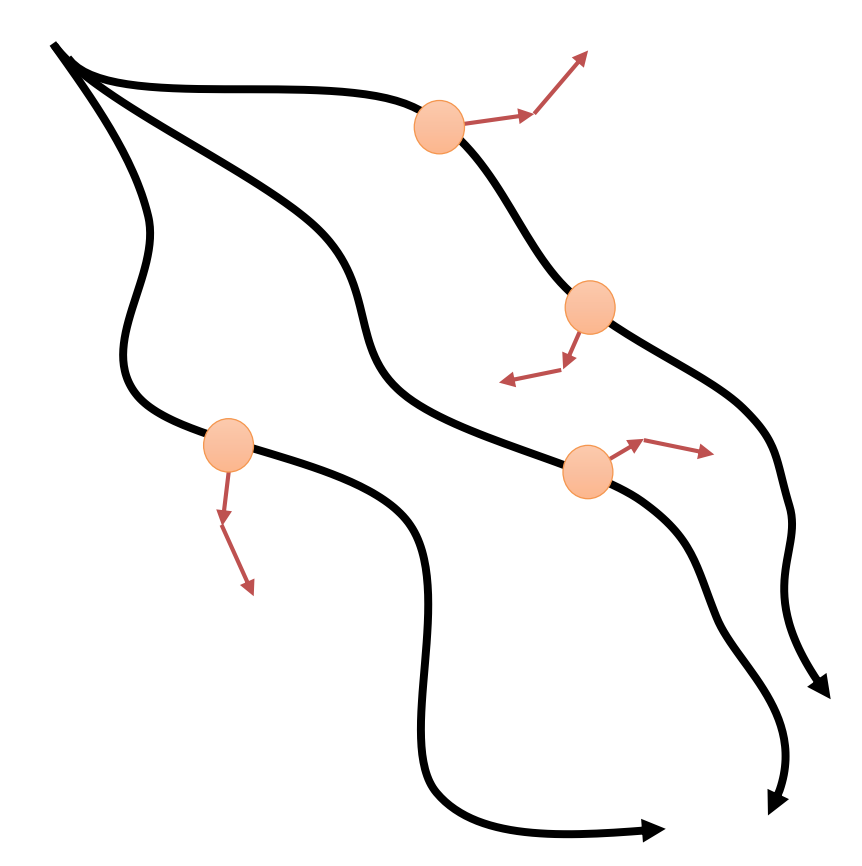
\includegraphics[scale=0.4]{figures/dynarollout.png}
    \caption{General Dyna training}
    \label{fig:dynarollout}
\end{figure}
As shown in Fig. \ref{alg:dynagen}, we choose some states (orange dots) from the buffer, simulate the next states using the learned model, and then train model-free RL with synthetic data $(s,a,s',r)$ where $s$ is from the experience buffer, $s'$ is from the learned model. One could also take more than one step if one believes that the model is good enough for more steps. 

This algorithm only requires very short (as few as one step) rollouts from model, so the mistakes will not exacerbate and accumulate much. Moreover, we explore well with a lot of samples because we still see diverse states. 

\section{Local and Global Models}
Recall that in LQR, we can turn a constrianed optimization problem into an unconstrained problem:
\[
\min_{u_1,\dots,u_T}c(x_1,u_1)+c(f(x_1,u_1),u_2)+\dots+c(f(f(\dots)\dots),u_T)
\]
Backpropagation is indeed a possible solution to solve this optimization problem, and we need $\frac{df}{d{x_t}}$, $\frac{df}{du_t}$, $\frac{dc}{dx_t}$, $\frac{dc}{du_t}$

\subsection{Local Models}
Since LQR gives us a state-feedback controller for a linear system, we can keep linearizing the system and iteratively apply LQR to generate local models. We fit $\frac{df}{d{x_t}}$, $\frac{df}{du_t}$ around the current trajectory or policy. Say the model is a Gaussian $p(x_{t+1}|x_t,u_t)=\mathcal{N}(f(x_t,u_t),\Sigma)$, then we can approximate the model as a linear function $f(x_t,u_t)\simeq A_t x_t+B_tu_t$, and we can use $\frac{df}{d{x_t}}$ as $A_t$, and $\frac{df}{du_t}$ as $B_t$.

Iterative LQR produces $\hat{x_t},\hat{u_t},K_t,k_t$, where $u_t = K_t(x_t-\hat{x_t})+k_t+\hat{u_t}$. We can execute the controller using a Gaussian $p(u_t|x_t) = \mathcal{N}(K_t(x_t-\hat{x_t})+k_t+\hat{u_t},\Sigma_t)$ because we can add noise to the iLQR controller so that all samples do not look the same. Practically, we can set $\Sigma_t = Q^{-1}_{u_t,u_t}$.
\begin{figure}
    \centering
    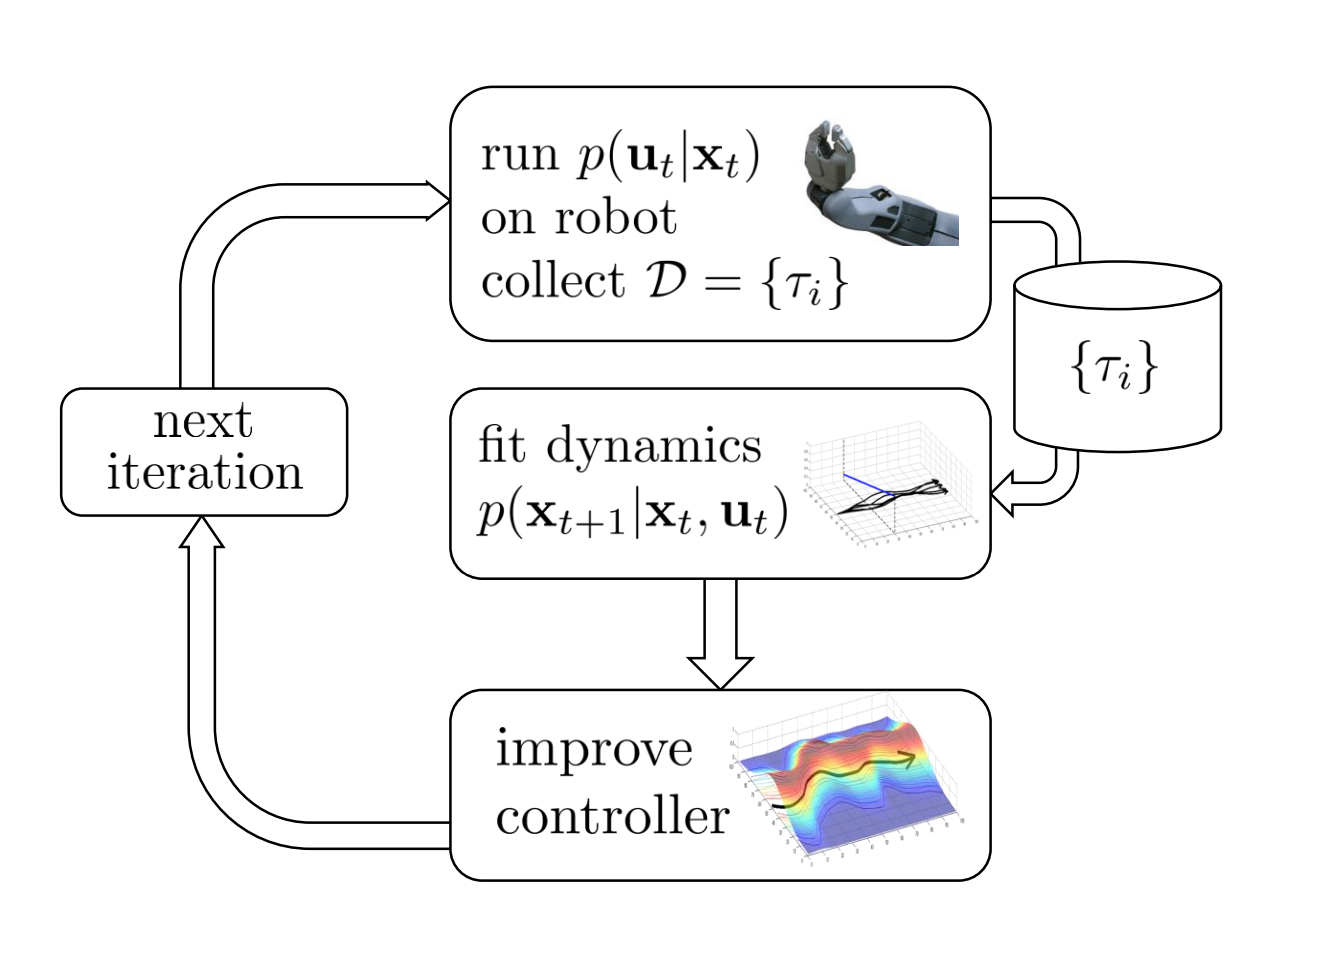
\includegraphics[scale=0.35]{figures/localmodel.png}
    \caption{Local models fitting}
    \label{fig:localmodel}
\end{figure}
We can fit the model $p(s_{t+1}|s_t,a_t)$ using Bayesian linear regression, and use the global model as prior.

We also need to stay close to old controller if we go too far. If trajectory distribution is close, then dynamics will be close too. Close here means the KL-divergence is small $D_{KL}(p(\tau)||p(\Bar{\tau}))\leq \epsilon$.

%todo: idk how fitting the dynamics works

\subsection{Guided Policy Search}
The high level idea of guided policy search is to use some simpler local policy such as local LQR controller to help and guide the learning process of more complex global policy learner. Essentially, we would use the local models trajectories as the training data for a supervised learning neural net that can solve all the tasks.

However, one problem is that the local policies might not be able to be reproduced using a single neural net. Therefore, after training the global policy with supervised learning, we need to reoptimize the local policies using the global policy so that the policies are consistent with each other. The sketch of guided policy search is shown in Alg. \ref{alg:guided}. Note that the cost function $\Tilde{c}_{k,i}$ is the modified cost function to keep $\pi_{LQR}$ close to $\pi_\theta$.
\begin{algorithm}[t!]
\caption{Guided Policy Search}
\begin{algorithmic}[1]
\label{alg:guided}
\WHILE{True}
\STATE Optimize each local policy $\pi_{LQR,i}(u_t|x_t)$ on initial state $x_{0,i}$ with respect to $\Tilde{c}_{k,i}(x_t,u_t)$
\STATE Use samples from the previous step to train $\pi_\theta(u_t|x_t)$ to mimic each $\pi_{LQR,i}(u_t|x_t)$
\STATE Update cost function $\Tilde{c}_{k+1,i}(x_t,u_t) = c(x_t,u_t) + \lambda_{k+1}\log \pi_\theta(u_t|x_t)$
\ENDWHILE
\end{algorithmic}
\end{algorithm}

In Divide and Conquer RL, the idea is similar, except that we are replacing the local LQR controllers with local neural net. 

\chapter{Variational Inference and Generative Models}
In this chapter we are going to explore some techniques that allow us to infer latent variables in latent space. We will try to understand the role of latent probabilistic models in deep learning and how to use them.

In RL, we are mostly concerned with conditional distributions $p(x|y)$ because we are trying to fit a policy function $\pi_\theta(a|s)$ which is a probabilistic model of action conditioned on state. 

So what are latent variable models? Consider that we have a very complicated distribution $p(x)$, which cannot be easily modeled by a mixture of Gaussians. By Bayes' rule, this complicated prior can be modeled by two other easier distributions:
\[
p(x) = \int p(x|z)p(z)dz
\]
$p(x|z)$ and $p(z)$ could be modeled by a conditional Gaussian and a Gaussian respectively. Since any function could be represented by a big enough neural network to an arbitrary precision, we can then use a neural net to represent $p(x|z)$ as $p(x|z) = \mathcal{N}(\mu_{nn}(z),\mu_{nn}(z))$. This sample distribution is a easy distribution with complicated parameters. Often in practice, we won't even learn $p(z)$, because we could just model it as a Gaussian distribution and transform it to any nonlinear distribution using the integral. The challenge of this approach, however, is to efficiently approximate the integral, which is quite hard.

In RL, we mainly use latent variable models in the following scenarios. First, we could use conditional latent variable models for multi-modal policies, as we discussed in imitation learning. Specifically, we could train a network with Gaussian noise to infer the state from image-based observations. Another scenario is that we could use latent variable models for model-based RL. Essentially, we learn a conditional distribution $p(o_t|x_t)$ and prior $p(x_t)$.

\section{Training Latent Variable Models}
The model we are trying to fit is $p_\theta(x)$. We train the model using data $\mathcal{D} = \{x_1,x_2,\dots,x_N\}$. We use maximum likelihood fit: $\theta\leftarrow \argmaxA_\theta\frac{1}{N}\sum_i\log p_\theta(x_i)$. Using latent variables, we have $\theta\leftarrow \argmaxA_\theta\frac{1}{N}\sum_i\log \left(\int p_\theta(x_i|z)p(z)dz \right)$. And as we have shown above, the integral is completely intractable. 

Alternatively, we could use the expected log-likelihhod:
\[
theta\leftarrow \argmaxA_\theta\frac{1}{N}\sum_i\mathbb{E}_{z\sim p(z|x_i)}\log p_\theta(x_i)
\]
However, the conditional distribution $p(z|x_i)$ is unknown. Therefore, we can approximate this distribution with a simpler distribution $q_i(z) =\mathcal{N}(\mu_i,\sigma_i)$.

\subsection{Variational Approximation}
It turns out that if we approximate the distribution using $q_i(z)$, we can bound the distribution of interest $\log p(x_i)$. Therefore, by maximizing this lower bound, we are maximizing the log likelihood. We use $q_i(z)$ to approximate $\log p(x_i)$ by:
\begin{align*}
    \log p(x_i) &= \log \int_z p(x_i|z)p(z)\\
    &= \log \int_z p(x_i|z)p(z)\frac{q_i(z)}{q_i(z)}\\
    &= \log\mathbb{E}_{z\sim q_i(z)}\left[\frac{p(x_i|z)p(z)}{q_i(z)}\right]\\
    &\geq \mathbb{E}_{z\sim q_i(z)}\left[\log \frac{p(x_i|z)p(z)}{q_i(z)}\right]\\
    &=\mathbb{E}_{z\sim q_i(z)}\left[\log p(x_i|z)+\log p(z)\right]-\mathbb{E}_{z\sim q_i(z)}\left[\log q_i(z)\right]\\
    &= \mathbb{E}_{z\sim q_i(z)}\left[\log p(x_i|z)+\log p(z)\right] + \mathcal{H}(q_i)
\end{align*}
where we applied Jensen's inequality in the second to last step. Jensen's inequality states that:
\[
\log \mathbb{E}[y] \geq \mathbb{E}[\log y]
\]

If we maximize $\log p(x_i|z)$, we will maximize $\log p(x_i)$. Also, intuitively, if we maximize $\log p(x_i|z)$, we are maximizing the peak of the distribution, and since we are maximizing the entropy $\mathcal{H}(q_i)$ too, we are also making the distribution as wide as possible, which is how we drive the approximated distribution $q_i(z)$ as close as possible to the target distribution $p(x_i,z)$.

Let us take a closer look at this lower bound. Define $\mathbb{E}_{z\sim q_i(z)}\left[\log p(x_i|z)+\log p(z)\right] + \mathcal{H}(q_i)$ as $\mathcal{L}_i(p,q_i)$. In tuitively, this term measures the likelihood. For a $q_i(z)$ to approximate $p(z|x_i)$ well, we need to minimize the KL-divergence between the two distributions. By definition, the KL divergence of the two distributions is written as:
\begin{align*}
    D_{KL}(q_i(x_i)||p(z|x_i))&=\mathbb{E}_{z\sim q_i(z)}\left[\log \frac{q_i(z)}{p(z|x_i)}\right]\\
    &=\mathbb{E}_{z\sim q_i(z)}\left[\log \frac{q_i(z)p(x_i)}{p(x_i,z)}\right]\\
    &= -\mathbb{E}_{z\sim q_i(z)}\left[\log p(x_i|z)+\log p(z)\right] + \mathbb{E}_{z\sim q_i(z)}\left[\log q_i(z)\right]+ \mathbb{E}_{z\sim q_i(z)}\left[\log p(x_i)\right]\\
    &= -\mathbb{E}_{z\sim q_i(z)}\left[\log p(x_i|z)+\log p(z)\right] -\mathcal{H}(q_i)+\log p(x_i)\\
    &=-\mathcal{L}_i(p,q_i) + \log p(x_i)
\end{align*}
Therefore,
\begin{align*}
    \log p(x_i) &= D_{KL}(q_i(z)||p(z|x_i)) + \mathcal{L}_i(p,q_i)\\
    \log p(x_i) &\geq \mathcal{L}_i(p,q_i)
\end{align*}
Note that we eliminated the expectation $\mathbb{E}_{z\sim q_i(z)}\left[\log p(x_i)\right]$ because $p(x_i)$ does not depend $z$.

Since $D_{KL}(q_i(x_i)||p(z|x_i)) = -\mathcal{L}_i(p,q_i) + \log p(x_i)$, maximizing $\mathcal{L}_i(p,q_i)$ with respect to $q_i$ minimizes the KL-divergence. Now in our maximum likelihood training, instead of doing $\theta \leftarrow \argmaxA_\theta \frac{1}{N}\sum_i \log p_\theta(x_i)$, we can use the lower bound and do $\theta \leftarrow \argmaxA_\theta \frac{1}{N}\sum_i \mathcal{L}_i(p,q_i)$ to approximate it. To optimize, for each $x_i$, we calculate $\nabla_\theta\mathcal{L}_i(p,q_i)$ by sampling $z\sim q_i(z)$ and the gradient of the likelihood term can be approximated using $\nabla_\theta\mathcal{L}_i(p,q_i)\simeq \nabla_\theta\log p_\theta(x_i|z)$ because $\log p_\theta(x_i|z)$ is the only term in the likelihood that depends on $\theta$. Then we apply gradient ascent on the parameter $\theta$ by $\theta \leftarrow \theta + \alpha\nabla_\theta\mathcal{L}_i(p,q_i)$.

However, we also need to update $q_i$ to maximize $\mathcal{L}_i(p,q_i)$ because it also depends on $\mathcal{H}(q_i)$. Let's say $q_i(z) = \mathcal{N}(\mu_i,\sigma_i)$, then we can apply gradient ascent on both parameters $\mu_i$, $\sigma_i$ to update this distribution. The problem here is the above update rule is for each data point. Therefore, the number of parameters is $|\theta| + (|\mu_i| + |\sigma_i|)*N$, where $N$ is the number of data points. Thus, we can modify the distribution we are learning so that we use a more general neural network to approximate $q(z|x_i)$ such that $q(z|x_i) = q_i(z)\simeq p(z|x_i)$. Now the number of the network parameter does not scale with the number of data points. 

\subsection{Amortized Variational Inference}
The above idea is called amortized variational inference. When we maximize the likelihood, instead of using $q_i$ for each data point, we use a general neural net $q_\phi$, parameterized by $\phi$. Then when we update $q_\phi$, we can just apply gradient ascent on $\phi$ by $\phi\leftarrow \phi + \alpha\nabla_\phi\mathcal{L}$. The likelihood can be denoted as $\mathcal{L}_i(p_\theta(x_i|z),q_\phi(z|x_i))$. 

How do we calculate $\nabla_\phi\mathcal{L}$? Note that 
\[
\mathcal{L}_i = \mathbb{E}_{z\sim q_\phi(z|x_i)}\left[\log p_\theta(x_i|z) + \log p(z)\right]+\mathcal{H}(q_\phi(z|x_i))
\]
to calculate the gradient of the likelihood with respect to $\phi$, we can calculate the entropy term's gradient easily using textbook formula. However, the first term is harder because the expectation is taken under a distribution depending on $\phi$, but the term inside the expectation is independent of $\phi$. Where have we seen this before? Where have seen the same type of gradient in policy gradient, and by applying the convenient identity, we can get the same form of gradient. If we call $\log p_\theta(x_i|z) + \log p(z)$ as $r(x_i,z)$, and $\mathbb{E}_{z\sim q_\phi(z|x_i)}$ as $J(\phi)$. Applying the same trick as in policy gradient, we can calculate $\nabla J(\phi)$ as:
\[
\nabla J(\phi)\simeq \frac{1}{M}\sum_j\nabla_\phi\log q_\phi(z_j|x_i)r(x_i,z_j)
\]
\subsection{The Reparameterization Trick}
Consider $q_\phi(z|x)$ as a Gaussian distribution $\mathcal{N}(\mu_\phi(x),\sigma_\phi(x))$, then for every $z$ in this distribution, it can be expressed as $z=\mu_\phi(x)+\epsilon\sigma_\phi(x)$, where $\epsilon$ is some type of a Gaussian noise $\epsilon \sim \mathcal{N}(0,1)$, and the noise is independent of $\phi$. Thus, we have:
\begin{align*}
    J(\phi) &= \mathbb{E}_{z\sim q_\phi(z|x_i)}[r(x_i,z)]\\
    &= \mathbb{E}_{\epsilon\sim \mathcal{N}(0,1)}\left[r(x_i,\mu_\phi(x)+\epsilon\sigma_\phi(x))\right]
\end{align*}
To estimate $\nabla_\phi J(\phi)$, we can just sample $M$ samples of $\epsilon$ from a Gaussian $\mathcal{N}(0,1)$.

Using this reparameterization trick, we can derive the expression of $\mathcal{L}_i$ in another way:
\begin{align*}
    \mathcal{L}_i &= \mathbb{E}_{z\sim q_\phi(z|x_i)}\left[\log p_\theta(x_i|z) + \log p(z)\right]+\mathcal{H}(q_\phi(z|x_i))\\
    &= \mathbb{E}_{z\sim q_\phi(z|x_i)}\left[\log p_\theta(x_i|z)\right] + \mathbb{E}_{z\sim q_\phi(z|x_i)}\left[\log p(z)\right] + \mathcal{H}(q_\phi(z|x_i))\\
    &=  \mathbb{E}_{z\sim q_\phi(z|x_i)}\left[\log p_\theta(x_i|z)\right] - D_{KL}(q_\phi(z|x_i)||p(z))\\
    &= \mathbb{E}_{\epsilon\sim \mathcal{N}(0,1)}\left[\log p_\theta(x_i|\mu_\phi(x_i)+\epsilon\sigma_\phi(x_i))\right] - D_{KL}(q_\phi(z|x_i)||p(z))\\
    &\simeq \log p_\theta( x_i|\mu_\phi(x_i)+\epsilon\sigma_\phi(x_i)) - D_{KL}(q_\phi(z|x_i)||p(z))
\end{align*}
The complete computational graph for variational inference is shown in Fig. \ref{fig:varinf}. 
\begin{figure}
    \centering
    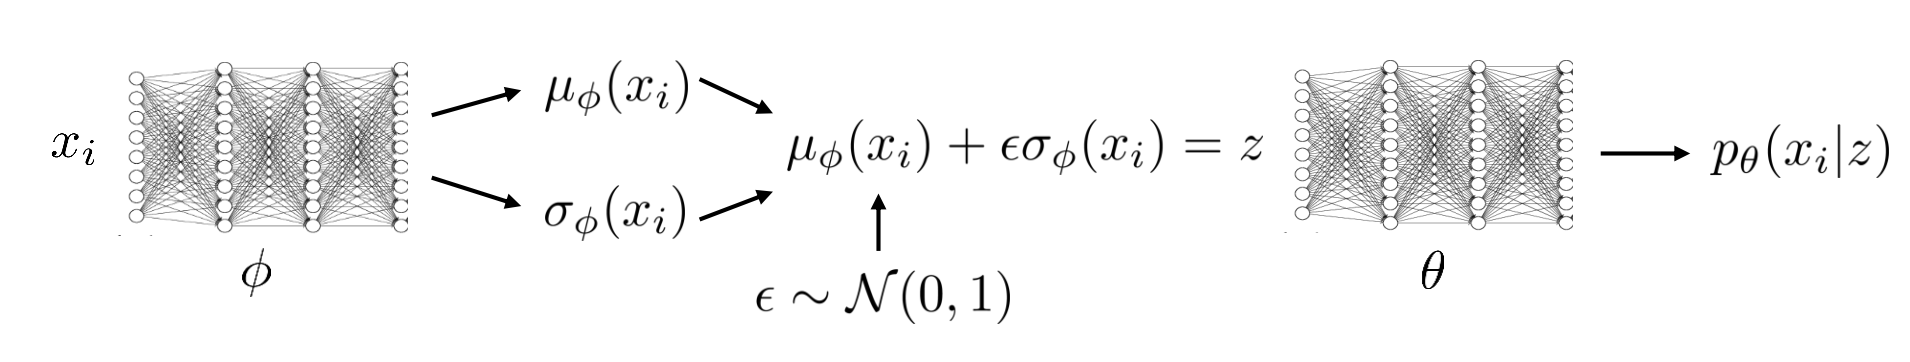
\includegraphics[scale=0.4]{figures/varinf.png}
    \caption{Variational inference}
    \label{fig:varinf}
\end{figure}

Compared with policy gradient, the reparameterization trick is easy to implement and as low variance, but it only works for continuous latent variables. Policy gradient can Can handle both discrete and continuous latent variables, but it is subject to high variance, rand equires multiple samples and small learning rates.

\section{Variational Autoencoder (VAE)}
The variational autoencoder (VAE) consists of two parts: an encoder and a decoder. The encoder $q_\phi(z|x) = \mathcal{N}(\mu_\phi(x),\sigma_\phi(x))$ parameterized by $\phi$ gives us a latent variable $z$, and the decoder $p_\theta(x|z) = \mathcal{N}(\mu_\theta(x),\sigma_\theta(x))$ is parameterized by $\theta$.

When we are inferring $p(x)$ by $p(x) = \int p(x|z)p(z)dz$, we sample $z$ from the distribution $p(z)$, and sample $x$ from the distribution $p(x|z)$. Why does this work? Recall the evidence lower bound $\mathcal{L}_i$ is defined as:
\[
\mathcal{L}_i=  \mathbb{E}_{z\sim q_\phi(z|x_i)}\left[\log p_\theta(x_i|z)\right] - D_{KL}(q_\phi(z|x_i)||p(z))
\]
$q_\phi$ should embed your observations $x_i$ into $z$, into a distribution that is closer to the prior. So if the training data is embedded into the distribution that is similar to the prior, it makes sense that the samples from the prior will give you things that look like the data.
\begin{figure}[H]
    \centering
    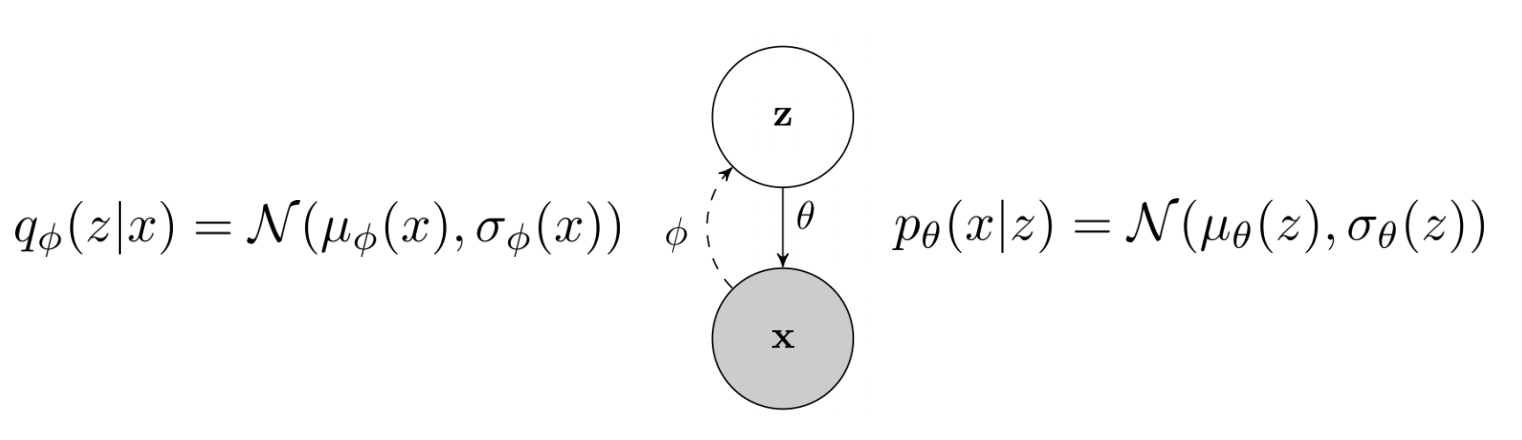
\includegraphics[scale=0.4]{figures/vae.png}
    \caption{VAE}
    \label{fig:vae}
\end{figure}
\chapter{Control as Inference}
In this chapter, we will talk about how we derive optimal control, reinforcement learning, and planning as
probabilistic inference. In a lot of scenarios that, say, involve biological behaviors, the data is not optimal. The behavior of the agent might be stochastic, but good behaviors are still more likely. 

\section{Probabilistic Graphical Model of Decision Making}
When we do not make any assumption of optimal behavior, we cannot ensure that the actions are chosen optimally. In other words, we cannot assume the following relation:
\[
a_1,\dots,a_T = \argmaxA_{a_1,\dots,a_T}\sum_{t=1}^Tr(s_t,a_t)
\]
Instead, we should model the probability distribution of seeing a trajectory $p(\tau) = p(s_{1:T},a_{1:T})$. We also introduce a binary optimality variable $\mathcal{O}_t$, which represents if the agent if behaving optimally at time step $t$. Then we are interested in $p(\tau|\mathcal{O}_{1:T})$, where we infer the probability of the given trajectory given the agent is optimal at every time step.
\begin{figure}
    \centering
    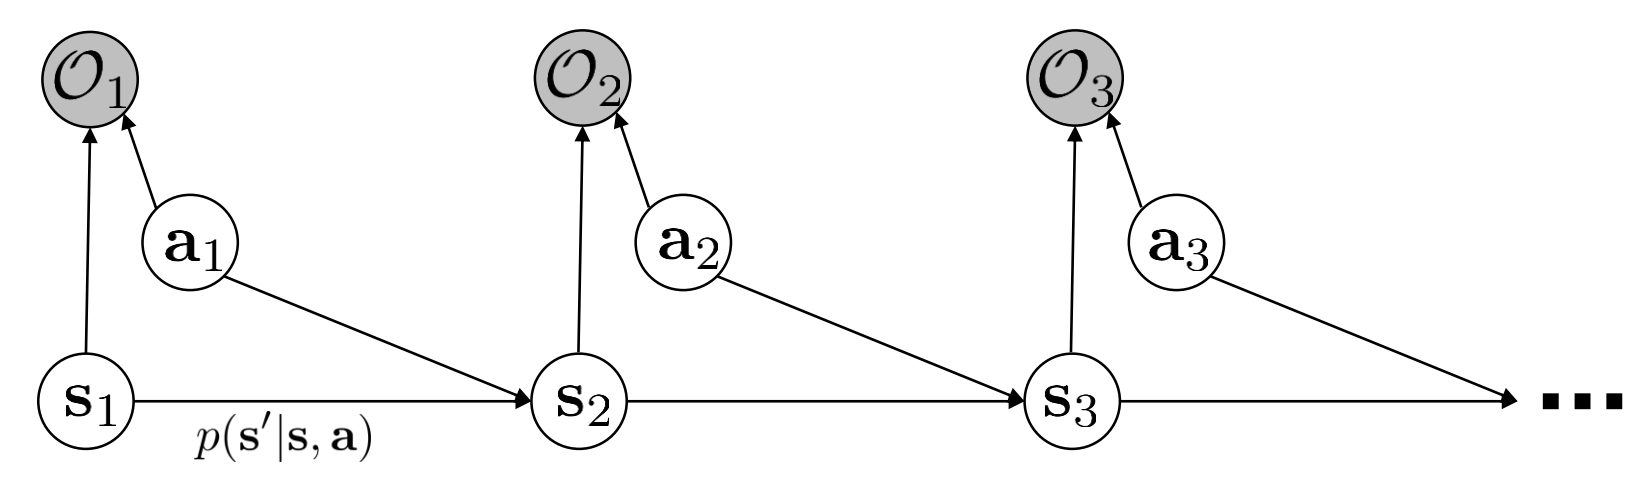
\includegraphics[scale=0.4]{figures/opt.png}
    \caption{Optimalility in stochastic behaviors}
    \label{fig:opt}
\end{figure}
Now we will model the optimality variable as follows: we model that the probability that variable is true given state and action is an exponential of the reward:
\[
p(\mathcal{O}_t|s_t,a_t) = \exp{r(s_t,a_t)}
\]
this might seem an arbitrary choice at the first sight, but we shall see later that this gives us an elegant mathematical expression in our derivation. We also assume for now that the reward function is always negative, but we can always take any reward function and normalize it by subtracting the max reward. Then by Bayes' Rule, we have:
\begin{align*}
    p(\tau|\mathcal{O}_{1:T}) &= \frac{p(\tau,\mathcal{O}_{1:T})}{p(\mathcal{O}_{1:T})}\\
    &\propto p(\tau)\prod_t \exp{r(s_t,a_t)}\\
    &= p(\tau)\exp{\sum_t r(s_t,a_t)}
\end{align*}
What does the above expression imply? Well, let us pretend that the dynamics are deterministic, then the first term $p(\tau)$ just means if this trajectory is possible. If not, then the probability is 0. If the trajectory is indeed possible, since we are multiplying by the exponent of the sum of rewards, then the probability of a trajectory given the agent is acting optimally is big with high rewards, but small with low rewards.

Let us take a look at the optimality model in Fig. \ref{fig:opt}. Why is this model important? Because the model is able to model suboptimal behavior, which is important for inverse RL that will be covered later. We then can apply inference algorithms to solve control and planning problems. It also provides an explanation for why stochastic behavior might be preferred, which is useful for exploration and transfer learning.

\subsection{Inference in the Optimality Model}
The first inference we will do is to compute the backward message $\beta_t(s_t,a_t) = p(\mathcal{O}_{t:T}|s_t,a_t)$, which means the probability of the agent being optimal from the current time step to the end given state and action. Another inference we will do is the policy $p(a_t|s_t,\mathcal{O}_{1:T})$. Note that we are inferring the possible actions taken given optimality. The last inference we do is the forward message $\alpha_t(s_t) = p(s_t|\mathcal{O}_{1:t-1})$, which is the probability of landing in a particular state given that the agent is acting optimally up to the current time step. 

\subsection{Inferring the Backward Messages}
The backward messages we are inferring is $\beta_t(s_t,a_t) = p(\mathcal{O}_{t:T}|s_t,a_t)$, which we will try to express in terms of transition probability $p(s_{t+1}|s_t,a_t)$ and optimality probability $p(\mathcal{O}_t|s_t,a_t)$. Mathematically, we can calculate $\beta_t(s_t,a_t)$ as:
\begin{align*}
    \beta_t(s_t,a_t)&=p(\mathcal{O}_{t:T}|s_t,a_t)\\
    &= \int p(\mathcal{O}_{t:T},s_{t+1}|s_t,a_t)ds_{t+1}\\
    &= \int p(\mathcal{O}_{t+1:T}|s_{t+1})p(s_{t+1}|s_t,a_t)p(\mathcal{O}_{t}|s_t,a_t)ds_{t+1}
\end{align*}
The second and the third terms in the product are known, so let us now focus on the first term:
\begin{align*}
p(\mathcal{O}_{t+1:T}|s_{t+1}) &= \int p(\mathcal{O}_{t+1:T}|s_{t+1},a_{t+1})p(a_{t+1}|s_{t+1})da_{t+1}\\
&=\int \beta(s_{t+1},a_{t+1})da_{t+1}
\end{align*}
we ignored $p(a_{t+1}|s_{t+1})$ it means which actions are likely a priori, and we assume it is uniform (constant) for now.

Therefore, to calculate the backward message, we have a recursive relation. For $t= T-1\;\text{to}\;1$:
\begin{align*}
    \beta_t(s_t,a_t) &= p(\mathcal{O}_{t}|s_t,a_t)\mathbb{E}_{s_{t+1}\sim p(s_{t+1}|s_t,a_t)}[\beta_{t+1}(s_{t+1})]\\
     \beta_t(s_t) &= \mathbb{E}_{a_{t}\sim p(a_t|s_t)}[\beta_t(s_t,a_t)]
\end{align*}

\subsection{A Closer Look}
Let us take a closer look at the backward pass. Let $V_t(s_t) = \log \beta_t(s_t)$, and let $Q_t(s_t,a_t) = \log \beta_t(s_t,a_t)$. Then 
$$V_t(s_t) = \log \int \exp (Q_t(s_t,a_t))da_t$$
As $Q_t(s_t,a_t)$ gets bigger $V_t(s_t)\rightarrow \max_{a_t}Q_t(s_t,a_t)$. Using the expression of $\beta_t(s_t,a_t)$, we will have
\[
Q_t(s_t,a_t) = r(s_t,a_t) + \log \mathbb{E}[\exp (V_{t+1}(s_{t+1}))]
\]

Recall in value iteration, we set $Q(s,a) \leftarrow r(s,a) + \gamma \mathbb{E}[V(s')]$. When the transition is deterministic, we have $Q_t(s_t,a_t) = r(s_t,a_t)+V_{t+1}(s_{t+1})$, which is similar to value iteration. However, when the transition is stochastic, then the $\log \exp$ term is like a maximum operation, so we have a biased optimistic estimation of the Q-function.

\subsection{Aside: The Action Prior}
Recall that we assumed $p(a_t|s_t)$ to be uniform, so it became constant in our integral. However, we shall see that it does not change much if the action prior is not uniform. Our V function now becomes $V_t(s_t) = \log \int \exp (Q_t(s_t,a_t)+\log p(a_t|s_t))da_t$, and our Q-function becomes $Q(s_t,a_t) = r(s_t,a_t) + \log p(a_t|s_t) + \log \mathbb{E}[\exp (V_{t+1}(s_{t+1}))]$
We can put the extra $p(a_t|s_t)$ into the reward term, then we will have the same expression of the Q-funtion, thus the V function. Therefore, uniform action prior can be assumed without loss of generality because it can always be folded into the reward.

\subsection{Inferring the Policy}
Now with backward messages available to us, we can then proceed to infer the policy $p(a_t|s_t,\mathcal{O}_{1:T})$. We derive the policy as follows:
\begin{align*}
    p(a_t|s_t,\mathcal{O}_{1:T}) &= \pi(a_t|s_t)\\
    &= p(a_t|s_t,\mathcal{O}_{t:T})\\
    &= \frac{p(a_t,s_t|\mathcal{O}_{t:T})}{p(s_t|\mathcal{O}_{t:T})}\\
    &= \frac{p(\mathcal{O}_{t:T}|a_t,s_t)p(a_t,s_t)/p(\mathcal{O}_{t:T})}{p(\mathcal{O}_{t:T}|s_t)p(s_t)/p(\mathcal{O}_{t:T})}\\
    &= \frac{p(\mathcal{O}_{t:T}|a_t,s_t)}{p(\mathcal{O}_{t:T}|s_t)}\frac{p(a_t,s_t)}{p(s_t)}\\
    &= \frac{\beta_t(s_t,a_t)}{\beta_t(s_t)}p(a_t|s_t)
\end{align*}
we discard the optimality variables $1,\dots t-1$ because then are conditionally independent of $s_t$. We also discard $p(a_t|s_t)$ since we can assume it as uniform. Using the definition of $V,Q$, we have
\begin{align*}
    \pi(a_t|s_t)&= \frac{\beta_t(s_t,a_t)}{\beta_t(s_t)}\\
    &= \exp(Q_t(s_t,a_t) - V_t(s_t))\\
    &= \exp(A_t(s_t,a_t))
\end{align*}
This result makes sense, because when we have large advantage function values, the action is more likely to be taken.

\subsection{Inferring the Forward Messages}
We now can infer our third task, the forward message $\alpha_t(s_t) = p(s_t|\mathcal{O}_{1:t-1})$. The derivation is as follows:
\begin{align*}
    \alpha_t(s_t) &= p(s_t|\mathcal{O}_{1:t-1})\\
    &= \int p(s_t,s_{t-1},a_{t-1}|\mathcal{O}_{1:t-1})ds_{t-1}da_{t-1}\\
    &= \int p(s_t|s_{t-1},a_{t-1},\mathcal{O}_{1:t-1})p(a_{t-1}|s_{t-1},\mathcal{O}_{1:t-1})p(s_{t-1}|\mathcal{O}_{1:t-1})ds_{t-1}da_{t-1}\\
    &= \int p(s_t|s_{t-1},a_{t-1})p(a_{t-1}|s_{t-1},\mathcal{O}_{t-1})p(s_{t-1}|\mathcal{O}_{1:t-1})ds_{t-1}da_{t-1}
\end{align*}
here we used the fact that the current state is conditionally independent of the previous optimality variables given the previous state, and we also used the fact that the current action is conditionally independent of the previous optimality variables given the current state. The first term is just the dynamics, so we need to figure out what the second and the third terms by Bayes' rule:
\begin{align*}
p(a_{t-1}|s_{t-1},\mathcal{O}_{t-1})p(s_{t-1}|\mathcal{O}_{1:t-1}) &= \frac{p(\mathcal{O}_{t-1}|s_{t-1},a_{t-1})p(a_{t-1}|s_{t-1})}{p(\mathcal{O}_{t-1}|s_{t-1})}\frac{p(\mathcal{O}_{t-1}|s_{t-1})p(s_{t-1}|p(\mathcal{O}_{1:t-2})}{p(\mathcal{O}_{t-1}|\mathcal{O}_{1:t-2})}\\
&=\frac{p(\mathcal{O}_{t-1}|s_{t-1},a_{t-1})p(a_{t-1}|s_{t-1})}{p(\mathcal{O}_{t-1}|\mathcal{O}_{1:t-2})}\alpha_{t-1}(s_{t-1})
\end{align*}
so now we have a recursive relation, and $\alpha_a(s_1) = p(s_1)$ is usually known. 

Another byproduct of having this forward message is that we can combine it with the backward message to calculate the probability of landing in a particular state given optimality variables:
\[
p(s_t|\mathcal{O}_{1:T})= \frac{p(s_t,\mathcal{O}_{1:T})}{p(\mathcal{O}_{1:T})} = \frac{p(\mathcal{O}_{t:T}|s_t)p(s_t,\mathcal{O}_{1:t-1})}{p(\mathcal{O}_{1:T})} \propto \beta_t(s_t)p(s_t|\mathcal{O}_{1:t-1})p(\mathcal{O}_{1:t-1})\propto\beta_t(s_t)\alpha_t(s_t)
\]

Geometrically, the relation between the state marginal and the product of backward and forward messages is shown in Fig. \ref{fig:marginal}. Here the backward messages is a backward cone, and the forward message is a forward cone. When we take the product of the two, we are essentially finding the intersection of the two cones. Intuitively, for a state in a trajectory, the state marginals are tighter near the beginning and the end, but looser near the center because the state marginals need to close in at the beginning and the end of a trajectory.
\begin{figure}
    \centering
    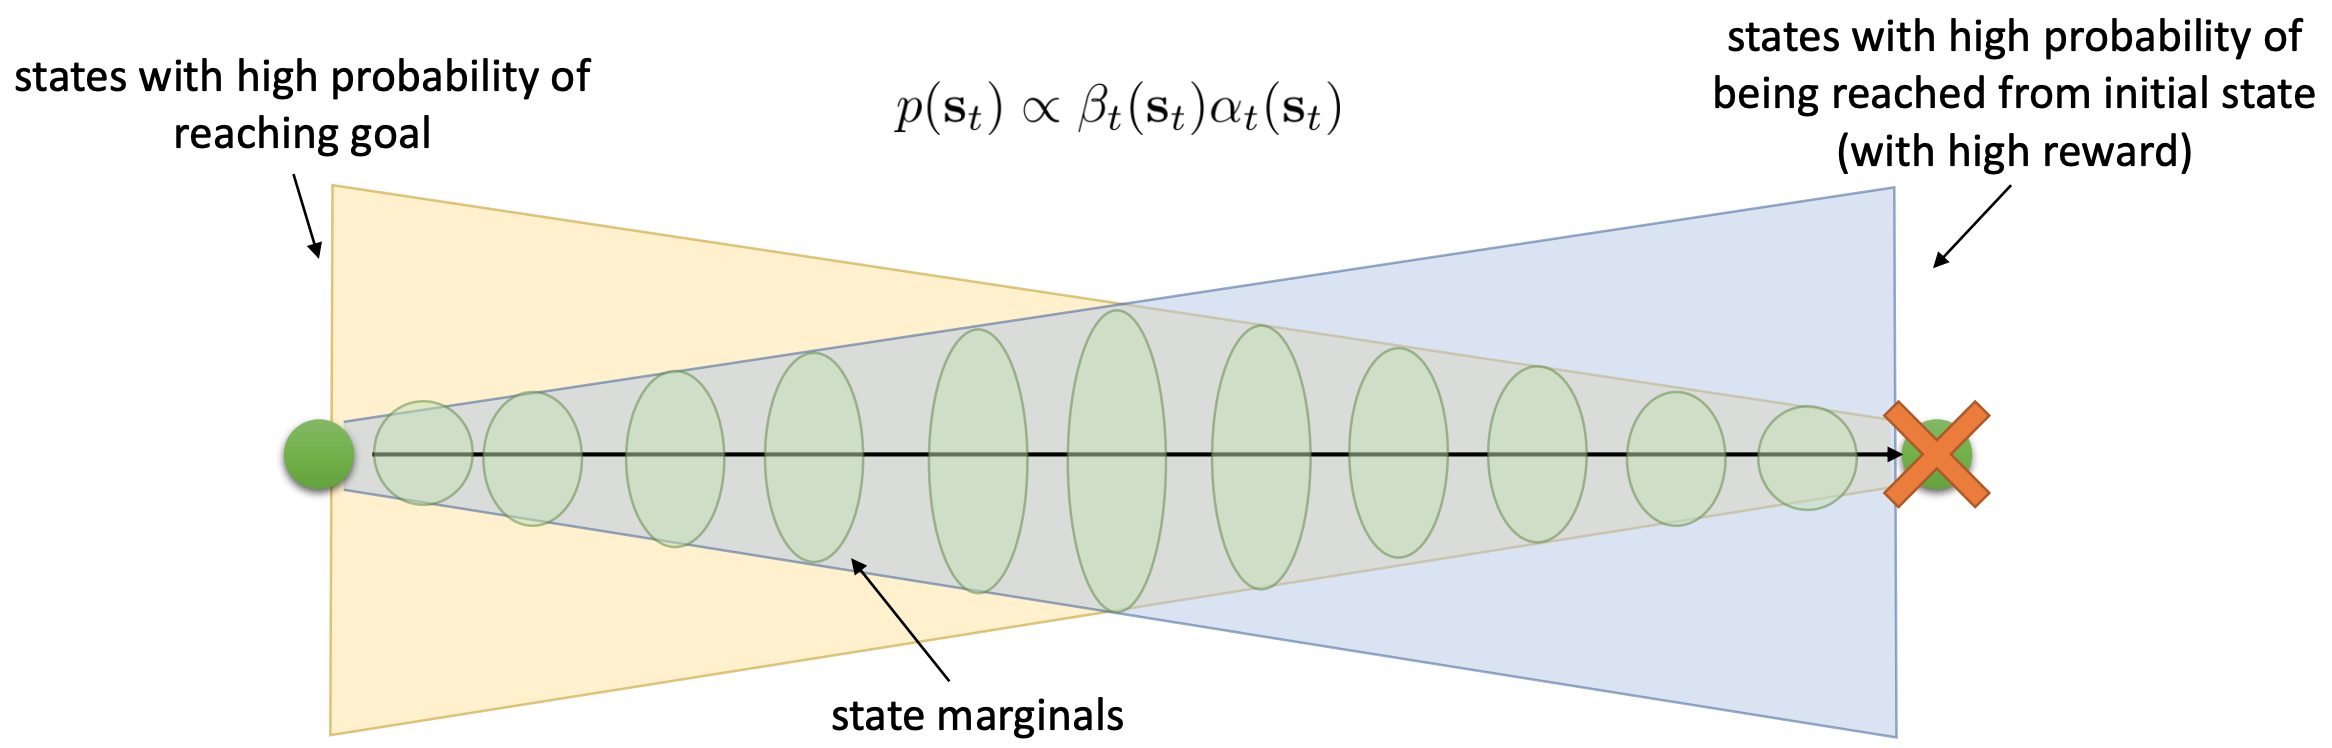
\includegraphics[scale=0.4]{figures/marginal.png}
    \caption{Forward/backward messages intersection}
    \label{fig:marginal}
\end{figure}

\section{The Optimism Problem}
Recall in the dynamic programming view of our backward message inference, the Q-function can be written as:
\[
Q_t(s_t,a_t) = r(s_t,a_t) + \log \mathbb{E}[\exp (V_{t+1}(s_{t+1}))]
\]
We have shown that $\log\mathbb{E}\exp$ behaves like a $\max$, thus bringing us bias in the estimate of Q-function. Marginalizing and conditioning the backward message $\beta_t(s_t,a_t) = p(\mathcal{O}_{t:T}|s_t,a_t)$, we can have two different distributions to infer: first, we can have the policy $p(a_t|s_t,\mathcal{O}_{1:T})$, which means given that you had a high reward (optimal), what was your action probability? Second, we can have the transition $p(s_{t+1}|s_t,a_t,\mathcal{O}_{1:T})$, and we should notice that this is not equal to the transition probability $p(s_{t+1}|s_t,a_t)$ because now we are asking given that you obtained high rewards, what was your transition probability? To address the optimism problem, we need to ask the first question: given that you obtained high reward, what was your action probability, assuming that we have the same transition probability, such that we are no luckier than we usually are. 

It turns out the first question is a difficult one. To answer that question, we can find another distribution $q(s_{1:T},a_{1:T})$ that is close to $p(s_t,a_t|\mathcal{O}_{1:T})$, but have the same $p(s_{t+1}|s_t,a_t)$. So let's us try variational inference. Let our evidence $x$, what we have observed, be the optimality variables $\mathcal{O}_{1:T}$, and the latent variable $z$, what we have not observed, be the trajectory $s_{1:T},a_{1:T}$. Using variational inference, we find a $q(z)$ to approximate $p(z|x)$.

Let $q(s_{1:T},a_{1:T}) = p(s_1)\prod_t p(s_{t+1}|s_t,a_t)q(a_t|s_t)$ since we are keeping the same initial state distribution and the same transition. Recall that the variational lower bound of the likelihood approximation is:
\[
\log p(x)\geq \mathbb{E}_{z\sim q(z)}[\log p(x,z) - \log q(z)]
\]
plugging in our previous definition of $q(z)$, we have
\begin{align*}
    \log p(\mathcal{O}_{1:T}) &\geq \mathbb{E}_{(s_{1:T},a_{1:T})\sim q}\bigg[ \log p(s_1) + \sum_{t=1}^T \log p(s_{t+1}|s_t,a_t) + \log p(\mathcal{O}_{T}|s_t,a_t)\\ &- \log p(s_1) - \sum_{t=1}^T \log p(s_{t+1}|s_t,a_t) - \sum_{t=1}^T\log q(a_t|s_t) \bigg]\\
    &= \mathbb{E}_{(s_{1:T},a_{1:T})\sim q}\left[\sum_t r(s_t,a_t) - \log q(a_t|s_t)\right]\\
    &= \mathbb{E}_{(s_{1:T},a_{1:T})\sim q}\left[r(s_t,a_t)+\mathcal{H}(q(a_t|s_t))\right]
\end{align*}
Therefore, to maximize the lower bound, we maximize the reward and the entropy.

%fill this in later
Using dynamic programming, we can get rid of the optimism $\max$ in the Bellman backup term.
\chapter{Inverse Reinforcement Learning}
So far in our RL algorithms, we have been assuming that the reward function is known a priori, or it is manually designed to define a task. What if we want to learn the reward function from observing an expert, and then use reinforcement learning? This is the idea of inverse RL, where we first figure out the reward function and then apply RL. 

Why should we worry about learning rewards at all? From the imitation learning perspective, the agent learns via imitation by copying the actions performed by the expert, without any reasoning about outcomes of actions. However, the natural way that human learn through imitation is that human copy the intent of the expert, and thus might take very different actions. In RL, it is often the case that the reward function is ambiguous in the environment. For example, it is hard to hand-design a reward function for autonomous driving. 

The inverse RL problem definition is as follows: we try to infer the reward functions from demonstrations, and then learn to maximize the inferred reward using any RL algorithm that was covered so far. Formally, in inverse RL, we learn $r_\psi(s,a)$, and then use it to learn $\pi^*(a|s)$. However, this is an underspecified problem, because many reward function can explain the same behavior. The reward function can take many forms. One potential form is the linear reward function, which is a weighted sum of features:
\[
r_\psi(s,a) = \sum_i\psi_if_i(s,a) = \psi^Tf(s,a)
\]
or it could be a neural net with parameters $\psi$.

\section{Feature Matching Inverse RL}
Let us focus on the linear reward function design for now. Since it is a weighted sum of features, one natural interpretation to match the features is to match the expectation of important features. Let $\pi^{r_\psi}$ be the optimal policy for reward function$r_\psi$, then we to design the reward, we are picking $\psi$ such that 
\[
\mathbb{E}_{\pi^{r_\psi}}[f(s,a)] = \mathbb{E}_{\pi^*}[f(s,a)]
\]
The right hand side expectation can be estimated using samples from expert: take $N$ samples of features, and get the average. The left hand side expectation is a little involved. One way to do it is to use any RL algorithm to maximize $r_\psi$, which is defined using the right hand side samples, and then produce $\pi^{r_\psi}$, and then we can use this policy to generate more samples. Another way is to use dynamic programming if we are given the transitions. To ensure the equality holds, we borrow some ideas from the support vector machine classifier, where we maximize the margin between the optimal policy's rewards and that of any other policy:
\[
\max_{\psi,m} m\;\;\text{s.t. }\;\psi^T\mathbb{E}_{\pi^*}[f(s,a)]\geq \max_{\pi\in \Pi}\psi^T\mathbb{E}_\pi[f(s,a)]+m
\]
but we also need to address the similarity between $\pi$ and $\pi^*$ so that similar policies do not need to abide by the $m$ margin requirement.

Using the SVM trick (with the use of Lagrangian dual), we can transform the above optimization into the following which also contains a function that measures the similarity between policies:
\[
\min_\psi \frac{1}{2}\lvert|\psi|\rvert^2\;\; \text{s.t. }\;\psi^T\mathbb{E}_{\pi^*}[f(s,a)]\geq \max_{\pi\in \Pi}\psi^T\mathbb{E}_\pi[f(s,a)]+D(\pi,\pi^*)
\]
where $D(\pi,\pi^*)$ measures the difference in feature expectations. However, such approaches have some issues: maximizing the margin is a bit arbitrary, and there is no clear model of expert suboptimality (can add slack variables). Furthermore, now we have a messy constrained optimization problem, which is not great for deep learning!

\section{Learning the Optimality Variable}
Recall that in last chapter, we introduced the optimality variable $\mathcal{O}_t$ to indicate if the agent is acting optimally. It turns out that as we learn the reward function, we are also learning the optimality variable. The optimality variable is defined as $p(\mathcal{O}_t|s_t,a_t) = \exp(r_\psi(s_t,a_t))$. Since the reward parameter $\psi$ is unknown, the optimality distribution should also depend on $\psi$: $p(\mathcal{O}_t|s_t,a_t,\psi)$. Recall that \[p(\tau|\mathcal{O}_{1:T},\psi)\propto\exp \left(\sum_tr_\psi(s_t,a_t)\right)\] Note that we can ignore $p(\tau)$ in our optimiztion since it does not depend on $\psi$. We are given sample trajectories $\{\tau_i\}$ sampled from expert policy $\pi^*(\tau)$, so the maximum likelihood training can be done using:
\[
\max_\psi\frac{1}{N}\sum_{i=1}^N\log p(\tau_i|\mathcal{O}_{1:T},\psi) = \max_\psi\frac{1}{N}\sum_{i=1}^N r_\psi(\tau_i)-\log Z
\]
where $Z$ is the \textbf{partition function} needed to make the sum of probability with respect to $\tau$ 1.

\subsection{Inverse RL Partition Function}
In our maximum likelihood training, to make the probability with respect to $\tau$ sum to 1, we introduced the IRL partition function $Z$. Mathematically, $Z$ is the integral of all possible trajectories:
\[
Z = \int p(\tau)\exp(r_\psi(\tau))d\tau
\]
Then we take the gradient of the likelihood with respect to $\psi$ after plugging in $Z$:
\begin{align*}
\nabla_\psi \mathcal{L} &= \frac{1}{N}\sum_{i=1}^N\nabla_\psi r_\psi(\tau_i) - \frac{1}{Z}\int p(\tau)\exp(r_\psi(\tau))\nabla_\psi r_\psi(\tau)d\tau\\
&= \mathbb{E}_{\tau\sim\pi^*(\tau)}[\nabla_\psi r_\psi(\tau_i)] - \mathbb{E}_{\tau\sim p(\tau|\mathcal{O}_{1:T},\psi)}[\nabla_\psi r_\psi(\tau)]
\end{align*}
The first expectation is estimated with expert samples, and the second expectation is the soft optimal policy under current reward. To increase the gradient, we want more expert trajectory and less current agent trajectory.

\subsection{Estimating the Expectation}
In the above derivation of the gradient of the likelihood, the first expectation is easy to calculate, but the second one is hard. To calculate the second expectation, we need to do some messaging:
\begin{align*}
    \mathbb{E}_{\tau\sim p(\tau|\mathcal{O}_{1:T},\psi)}[\nabla_\psi r_\psi(\tau)] &= \mathbb{E}_{\tau\sim p(\tau|\mathcal{O}_{1:T},\psi)}\left[\nabla_\psi\sum_{t=1}^Tr_\psi(s_t,a_t)\right]\\
    &= \sum_{t=1}^T\mathbb{E}_{(s_t,a_t)\sim p(s_t,a_t|\mathcal{O}_{1:T},\psi)}[\nabla_\psi r_\psi(s_t,a_t)]
\end{align*}
Note that the distribution $p(s_t,a_t|\mathcal{O}_{1:T},\psi)$ can be rewritten using chain rule as:
\[
p(s_t,a_t|\mathcal{O}_{1:T},\psi) = p(a_t|s_t,\mathcal{O}_{1:T},\psi)p(s_t|\mathcal{O}_{1:T},\psi)
\]
where 
\begin{align*}
    p(a_t|s_t,\mathcal{O}_{1:T},\psi) &= \frac{\beta(s_t,a_t)}{\beta(s_t)}\\
    p(s_t|\mathcal{O}_{1:T},\psi)&\propto\alpha(s_t)\beta(s_t)
\end{align*}
Therefore, the distribution is directly proportional to the product of the backward message and the forward message:
\[
p(a_t|s_t,\mathcal{O}_{1:T},\psi)p(s_t|\mathcal{O}_{1:T},\psi)\propto\beta(s_t,a_t)\alpha(s_t)
\]
If we let $\mu_t(s_t,a_t)\propto\beta(s_t,a_t)\alpha(s_t)$, then the second expectation can be written as:
\begin{align*}
\mathbb{E}_{\tau\sim p(\tau|\mathcal{O}_{1:T},\psi)}[\nabla_\psi r_\psi(\tau)] &= \sum_{t=1}^T\int \int \mu_t(s_t,a_t)\nabla_\psi r_\psi(\tau)ds_tda_t\\
&= \sum_{t=1}^T\mu_t^T\nabla_\psi r_\psi
\end{align*}
where $\mu_t$ is the state-action visitation probability for each $(s_t,a_t)$.

Now we are ready to sketch out our MaxEnt Inverse RL algorithm in Alg. \ref{alg:maxent}. We can use this to learn the reward function.
\begin{algorithm}[t!]
\caption{MaxEnt Inverse RL}
\begin{algorithmic}[1]
\label{alg:maxent}
\REQUIRE Some random reward parameter $\psi$
\WHILE{True}
\STATE Given $\psi$, compute backward message $\beta(s_t,a_t)$
\STATE Given $\psi$, compute forward message $\alpha(s_t)$
\STATE Compute $\mu_t(s_t,a_t)\propto \beta(s_t,a_t)\alpha(s_t)$
\STATE Evaluate $\nabla_{\psi}\mathcal{L} = \frac{1}{N}\sum_{i=1}^N\sum_{t=1}^T\nabla_\psi r_\psi(s_{i,t},a_{i,t}) -\sum_{t=1}^T\int \int \mu_t(s_t,a_t)\nabla_\psi r_\psi(\tau)ds_tda_t$
\STATE $\psi \leftarrow \psi + \eta\nabla_\psi\mathcal{L}$
\ENDWHILE
\end{algorithmic}
\end{algorithm}
Why is it called maximum entropy (MaxEnt)? Because in cases where $r_\psi(s_t,a_t) = \psi^Tf(s_t,a_t)$, we can show that Alg. \ref{alg:maxent} oprimizes
\[
\max_\psi\mathcal{H}(\pi^{r_\psi})\;\text{s.t. }\;\;
\mathbb{E}_{\pi^{r_\psi}}[f] = \mathbb{E}_{\pi^*}[f]
\]

\section{Unknown Dynamics and Large State/Action Spaces}
So far, MaxEnt inverse RL requires us to solve for a soft optimal policy in the inner loop, and it enumerates all state-action tuples for visitation frequency and gradient. To apply the IRL algorithms in practical problem settings, we need to handle large and continuous state and action spaces and unknown dynamics.

Recall the gradient of likelihood is calculated as
\[
\nabla_\psi \mathcal{L} =\mathbb{E}_{\tau\sim\pi^*(\tau)}[\nabla_\psi r_\psi(\tau_i)] - \mathbb{E}_{\tau\sim p(\tau|\mathcal{O}_{1:T},\psi)}[\nabla_\psi r_\psi(\tau)]
\]
We know that the first expectation is easy to calculate by sampling expert data, but the second expectation which is taken under the soft optimal policy under current reward is hard to calculate. One idea to calculate it is to learn the entire soft optimal policy $p(a_t|s_t,\mathcal{O}_{1:T},\psi)$ using any max-ent RL algorithm and then run this policy to sample $\{\tau_j\}$ such that:
\[
\nabla_\psi \mathcal{L} = \frac{1}{N}\sum_{i=1}^N\nabla_\psi r_\psi(\tau_i) - \frac{1}{M}\sum_{j=1}^M\nabla_\psi r_\psi(\tau_j)
\]
where we estimate the second expectation using the current policy samples. However, this is highly impractical because this requires us to run an RL algorithm to convergence in every gradient step.
\subsection{More Efficient Updates}
As mentioned above, learning $p(a_t|s_t,\mathcal{O}_{1:T},\psi)$ in the inner loop in each time step is expensive. Therefore, we can relax this objective a little to make it more efficient: instead of learning the policy at each time step, we could improve the policy a little in each time step such that if the policy keeps getting better, we can generate good samples eventually. Now sampling from this improved distribution is not actually sampling from the distribution we want, which is $p(\tau|\mathcal{O}_{1:T},\psi)$, we are actually getting a biased estimate of the distribution. Therefore, to resolve this issue, we use importance sampling:
\begin{align*}
    \nabla_\psi \mathcal{L} &\simeq \frac{1}{N}\sum_{i=1}^N\nabla_\psi r_\psi(\tau_i) - \frac{1}{\sum_j w_j}\sum_{j=1}^M w_j\nabla_\psi r_\psi(\tau_j)\\
    w_j &= \frac{p(\tau)\exp(r_\psi(\tau_j))}{\pi(\tau_j)}
\end{align*}
And if we take a closer look at the importance ratio $w_j$:
\begin{align*}
     w_j &= \frac{p(\tau)\exp(r_\psi(\tau_j))}{\pi(\tau_j)}\\
     &= \frac{p(s_1)\prod_t p(s_{t+1}|s_t,a_t\exp(r_\psi(s_t,a_t))}{p(s_1)\prod_t p(s_{t+1}|s_t,a_t\pi(a_t|s_t)}\\
     &= \frac{\exp(\sum_tr_\psi(s_t,a_t))}{\prod_t\pi(a_t|s_t)}
\end{align*}
With the importance ratio, each policy update with respect to $r_\psi$ brings us closer to the target distribution.

\section{Inverse RL as a Generative Adversarial Network}
The idea of inverse RL looks like a game. Specifically, we have an initial policy $\pi_\theta$, and expert demonstrations $\pi^*$. We sample trajectories $\tau_j$ from the initial policy, and $\tau_i$ from the expert policy. Then our gradient step looks like:
\[
\nabla_\psi \mathcal{L} \simeq \frac{1}{N}\sum_{i=1}^N\nabla_\psi r_\psi(\tau_i) - \frac{1}{\sum_j w_j}\sum_{j=1}^M w_j\nabla_\psi r_\psi(\tau_j)
\]
where demos are made more likely and samples are made less likely. Then we update the initial policy $\pi_\theta$ with respect to $r_\psi$:
\[
\nabla_\theta\mathcal{L}\simeq \frac{1}{M}\sum_{j=1}^M\nabla_\theta \log \pi_\theta(\tau_j)r_\psi(\tau_j)
\]
which in turn changes the policy to make it harder to distinguish from demos.

This looks a lot like a GAN. In a GAN, we have a generator that takes in some noise $z$, and outputs a distribution $p_\theta(x|z)$. We sample from the generator distribution $p_\theta(x)$. There is also demonstration data, for example, the real images, which we sample from its distribution $p^*(x)$. There is a discriminator parameterized by $\psi$ that determines if the data generated by the generator is real: $D(x) = p_\psi(\text{real}|x)$. We update the discriminator parameter by maximizing the binary log likelihood:
\[
\psi = \argmaxA_\psi \frac{1}{N}\sum_{x\sim p^*}\log D_\psi(x) + \frac{1}{M}\sum_{x\sim p_\theta}\log(1-D_\psi(x))
\]
where the log likelihood of the data is from demonstration is maximized and that of the data is from generator is minimized. We also update the generator parameter $\theta$:
\[
\theta\leftarrow \argmaxA_\theta \mathbb{E}_{x\sim p_\theta}\log D_\psi(x)
\]
so as to make it harder to distinguish from demos.

Therefore, interestingly, we can frame the IRL problem as a GAN. In a GAN, the optimal discriminator can be defined as:
\[
D^*(x) = \frac{p^*(x)}{p_\theta(x) + p^*(x)}
\]
For inverse RL, the optimal policy approaches $\pi_\theta(\tau)\propto p(\tau)\exp(r_\psi(\tau))$. Choosing the above optimal parameterization of the discriminator:
\begin{align*}
    D_\psi(\tau) &= \frac{p(\tau)\frac{1}{Z}\exp(r(\tau))}{p_\theta(\tau) + p(\tau)\frac{1}{Z}\exp(r(\tau))}\\
    &= \frac{p(\tau)\frac{1}{Z}\exp(r(\tau))}{p(\tau)\prod_t\pi_\theta(a_t|s_t) + p(\tau)\frac{1}{Z}\exp(r(\tau))}\\
    &= \frac{\frac{1}{Z}\exp(r(\tau))}{\prod_t\pi_\theta(a_t|s_t) + \frac{1}{Z}\exp(r(\tau))}
\end{align*}
then we optimize the discriminator with respect to $\psi$ such that:
\[
\psi \leftarrow \argmaxA_\psi \mathbb{E}_{\tau\sim p^*}[\log D_\psi(\tau)] + \mathbb{E}_{\tau\sim \pi_\theta}[\log (1-D_\psi(\tau))]
\]
Now we don't need the importance ratio anymore, because it is subsumed into $Z$.

We could also use a general discriminator, where $D_\psi$ is just a normal binary neural net classifier. It is often simpler to set up optimization, because we have fewer moving parts. However, the discriminator knows nothing at convergence generally cannot reoptimize the reward.
% TODO: know what it actually means
\bibliographystyle{IEEEtran}
\bibliography{IEEEabrv,ref}
\end{document}
